\documentclass[landscape,9pt]{beamer}
\usepackage{beamerthemeshadow}
\setbeamertemplate{navigation symbols}{}
\usepackage{natbib}
\bibpunct[:]{(}{)}{;}{a}{}{,}
\def\newblock{\hskip .11em plus .33em minus .07em}
\bibliographystyle{../yahapj}
\usepackage{graphicx}
\usepackage{comment}
\usepackage{../aastex_hack}
\usepackage{tikz}


\title[Exploring Quasar SEDs]{Spectral Energy Distributions, Dust, \\and Black Hole Properties: \\A Statistical, Multi-Wavelength Quasar Analysis}
\titlegraphic{\vspace{-2.5cm}\hspace{-.8\textwidth}
\includegraphics[width=.2\textwidth]{../images/Talk/logo_drexel}}
\author{Coleman Krawczyk}
\institute{Drexel University}
\date{9/4/2014}

\begin{document}

\frame{\titlepage}

\section{Introduction}
\subsection{The Basics}

\begin{frame}
	%\vspace{-2.19mm}
	\begin{columns}
	\begin{column}{.6\textwidth}
		\includegraphics<1->[width=\textwidth]{../images/Talk/agn_03}
	\end{column}
	\begin{column}{.5\textwidth}
		\begin{block}{What is a quasar?}
		\begin{itemize}
			\item A super massive black hole at the center of a distant galaxy that is actively accreting material
			\item This accretion process is so luminous that it can outshine all the stars in the host galaxy
			\item Quasar appear as point sources
			\item Some quasars have powerful radio jets
		\end{itemize}
		\end{block}
	\end{column}
	\end{columns}
\end{frame}

\begin{frame}
	\makebox[\textwidth][c]{
	\begin{tikzpicture}
		\node[anchor=south west,inner sep=0] (image) at (0,0) {\includegraphics<1->[width=.6\textwidth]{../images/Talk/agn_03}};
		\node[anchor=south west,inner sep=0] (sed) at (6.5,0) {\includegraphics<1-4>[width=.55\textwidth]{../images/Talk/elvis_94_mean}};
		\node[anchor=south west,inner sep=0] (spec) at (6.5,-.5) {\includegraphics<5->[width=.55\textwidth]{../images/Talk/vandenberk_01}};
		\node[anchor=north west,inner sep=0] (text) at (0,6.75) {	
		\begin{columns}
		\begin{column}{.75\textwidth}
		\end{column}
		\begin{column}{.45\textwidth}
		\begin{block}{What makes up a quasar?}
			\begin{itemize}
				\only<1>{\item The corona near the black hole produces emission in the X-ray ($\sim$AU)}
				\only<2>{\item The accretion disk produces thermal emission in the optical--UV ($\sim$1000\,AU)}
				\only<3>{\item The dusty torus absorbs the UV light and reemits it in the IR ($\sim$pc)}
				\only<4>{\item In radio loud quasars the jets produce synchrotron radiation ($\sim$100\,kpc)}
				\only<5>{\item Ionized gas within the potential well of the black hole create broad emission lines ($\sim$pc)}
				\only<6>{\item Ionized gas outside the potential well of the black hole create narrow emission lines ($\sim$kpc)}
			\end{itemize}
		\end{block}
		\end{column}
		\end{columns}
		};
		%\draw[help lines,xstep=1,ystep=1] (0,0) grid (12,7);
		\begin{scope}[x={(image.south east)},y={(image.north west)}]
			%\draw[help lines,xstep=.1,ystep=.1] (0,0) grid (1,1);
			\draw<1>[red,ultra thick,rotate around={-28:(.52,.51)}] (.52,.51) ellipse (.03 and .02);
			\draw<2>[red,ultra thick,rotate around={-28:(.52,.51)}] (.52,.51) ellipse (.25 and .07);
			\draw<3>[red,ultra thick] (.8,.3) circle (.1);
			\draw<4>[red,ultra thick,rotate around={63:(.65,.75)}] (.65,.75) ellipse (.3 and .07);
			\draw<5>[red,ultra thick] (.8,.63) circle (.1);
			\draw<6>[red,ultra thick] (.9,.9) circle (.08);
		\end{scope}
		\begin{scope}[shift=(sed.south west),x={(sed.south east)},y={(sed.north west)}]
			%\draw<1-4>[help lines,xstep=.1,ystep=.1] (0,0) grid (1,1);
			\draw<1>[red,ultra thick] (.9,.72) ellipse (.09 and .05);
			\draw<2>[red,ultra thick,rotate around={28:(.65,.8)}] (.65,.8) ellipse (.07 and .05);
			\draw<3>[red,ultra thick] (.5,.75) ellipse (.1 and .1);
			\draw<4>[red,ultra thick] (.15,.35) ellipse (.06 and .25);
			\node<1-4>[anchor=south east,inner sep=0] at (.95,0) {\tiny \citet{Elvis:1994}};
		\end{scope}
		\begin{scope}[shift=(spec.south west),x={(spec.south east)},y={(spec.north west)}]
			%\draw<5->[help lines,xstep=.1,ystep=.1] (0,0) grid (1,1);
			\draw<5>[red,thick,->] (.26,.15) -- (.26,.615);
			\draw<5>[red,thick,->] (.34,.15) -- (.34,.58);
			\draw<5>[red,thick,->] (.41,.15) -- (.41,.51);
			\draw<5>[red,thick,->] (.55,.15) -- (.55,.42);
			\draw<6>[red,thick,->] (.77,.8) -- (.77,.5);
			\node<5->[anchor=south east,inner sep=0] at (.95,0) {\tiny \citet{Vanden-Berk:2001}};
		\end{scope}
	\end{tikzpicture}
	}
\end{frame}

\subsection{SEDs}
\begin{frame}
	\begin{columns}
	\begin{column}{1.13\textwidth}
	\begin{block}{\citet{Elvis:1994} mean SEDs and uncertainties}
	\begin{columns}
		\begin{column}{0.4\textwidth}
			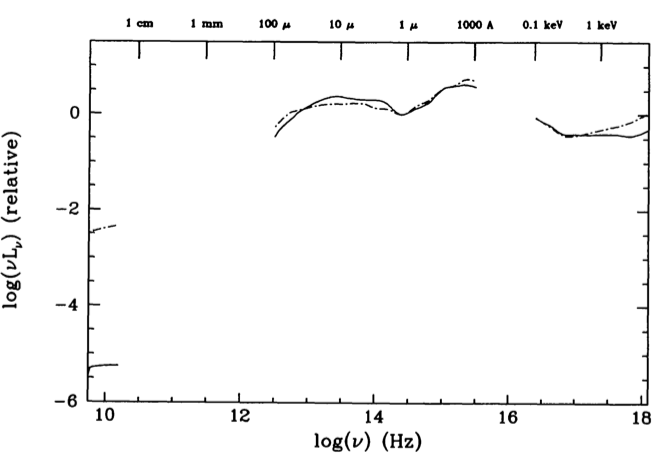
\includegraphics[width=\textwidth]{../images/Talk/elvis_94_mean}
		\end{column}
		\begin{column}{0.45\textwidth}
			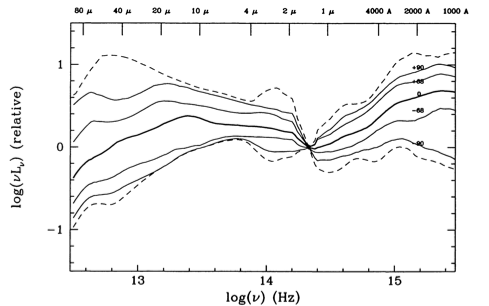
\includegraphics[width=\textwidth]{../images/Talk/elvis_94_unc}
		\end{column}
	\end{columns}
	\vspace{5mm}
	``...the large dispersion of shapes in individual objects means that the mean SED should be used only with caution, 
	   and that the variety of shapes should contain information about the physics of quasars.''
	\end{block}
	\end{column}
	\end{columns}
\end{frame}

\section{Data}
\begin{frame}
	\begin{columns}
	\begin{column}{.7\textwidth}
		\includegraphics<1>[width=\textwidth]{../images/Talk/opt_filts}
		\includegraphics<2>[width=\textwidth]{../images/Talk/uv_filts}
		\includegraphics<3>[width=\textwidth]{../images/Talk/nir_filts}
		\includegraphics<4>[width=\textwidth]{../images/Talk/mir_filts}
	\end{column}
	\begin{column}{.4\textwidth}
		\only<1>{
			\centering
			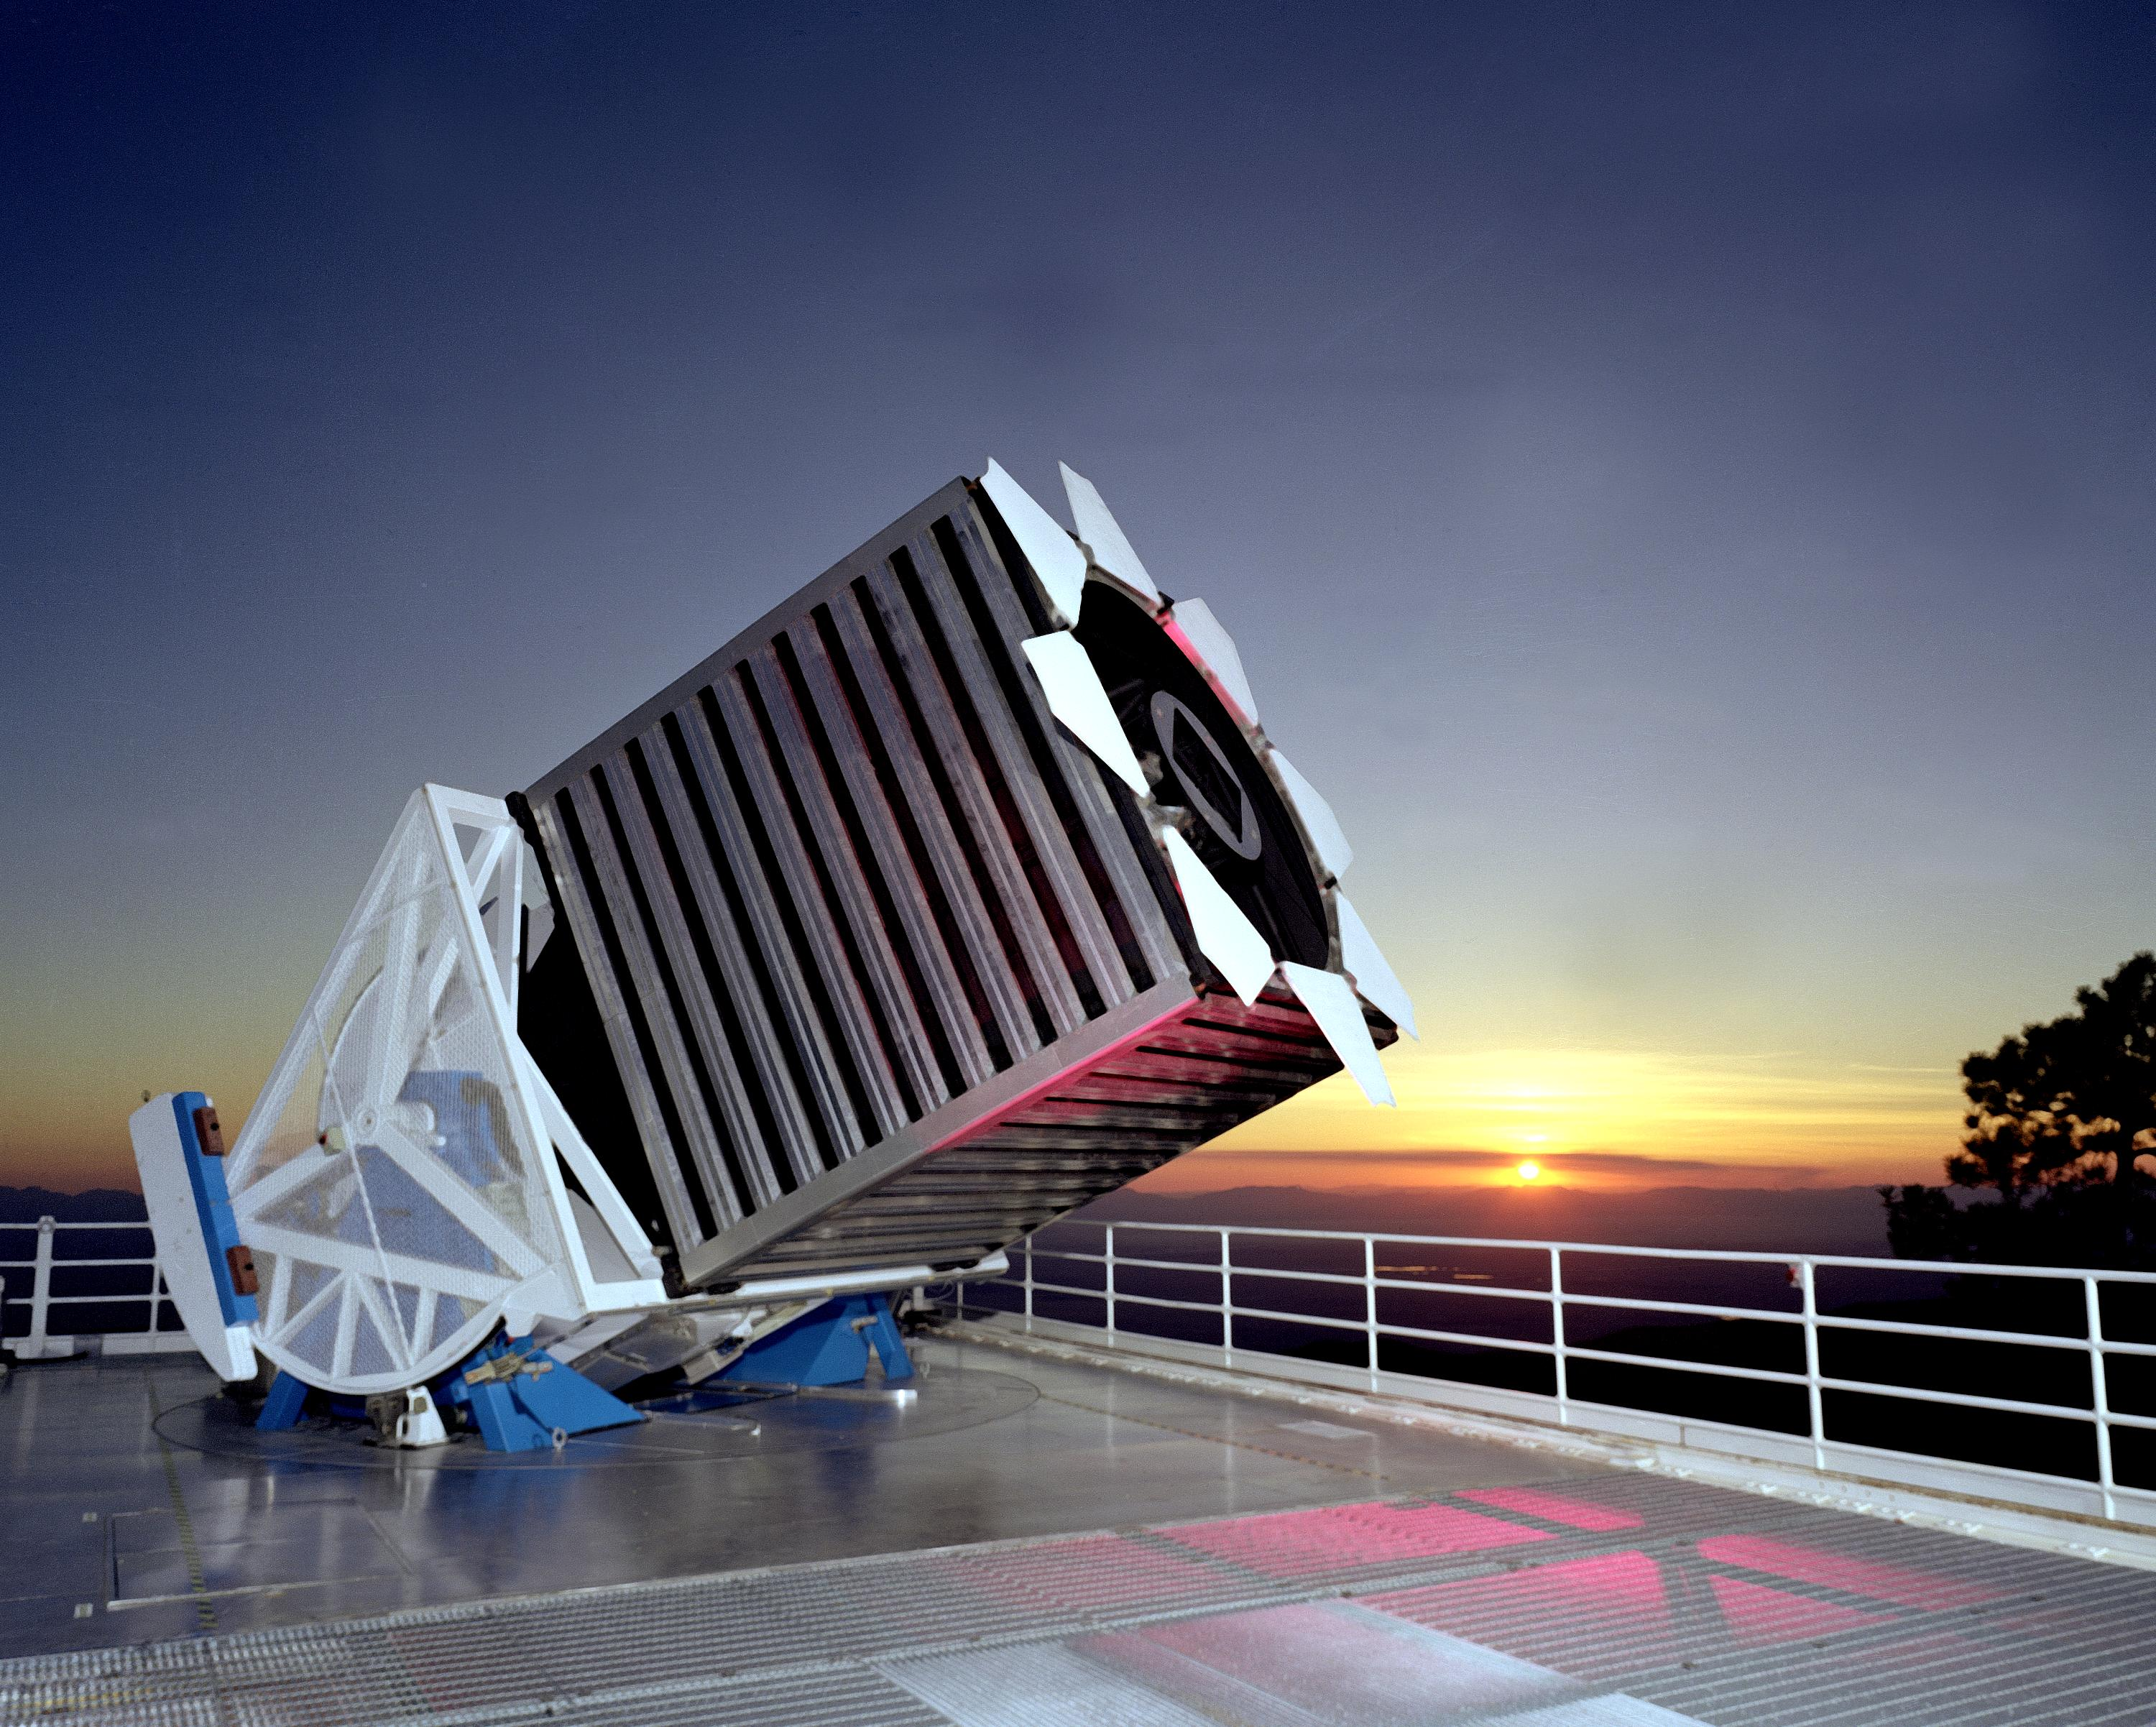
\includegraphics[width=.75\textwidth]{../images/Talk/sdss-telescope}
			\begin{block}{Optical}
				\begin{itemize}
					\item Our sample is taken from the SDSS DR7 quasar catalog containing 105,783 broad-lined quasars
					\item We supplement this sample with 15,757 lower luminosity quasars from various other studies
				\end{itemize}
			\end{block}}
		\only<2>{
			\centering
			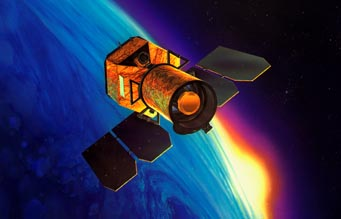
\includegraphics[width=.75\textwidth]{../images/Talk/Galex_art}
			\begin{block}{Ultra Violet}
				\begin{itemize}
					\item In the UV our sample was matched to {\em GALEX} data \citep{Budavari:2009}
					%\item Forced photometry was used to increase the number of matches to 42,046
				\end{itemize}
			\end{block}}
		\only<3>{
			\centering
			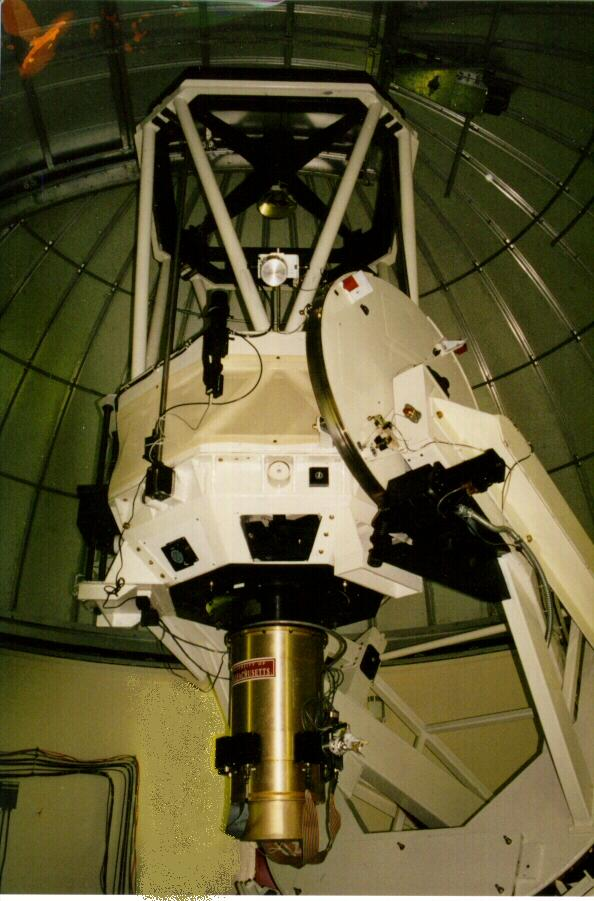
\includegraphics[angle=-90, origin=rb, width=.5\textwidth]{../images/Talk/2mass_telescope}
			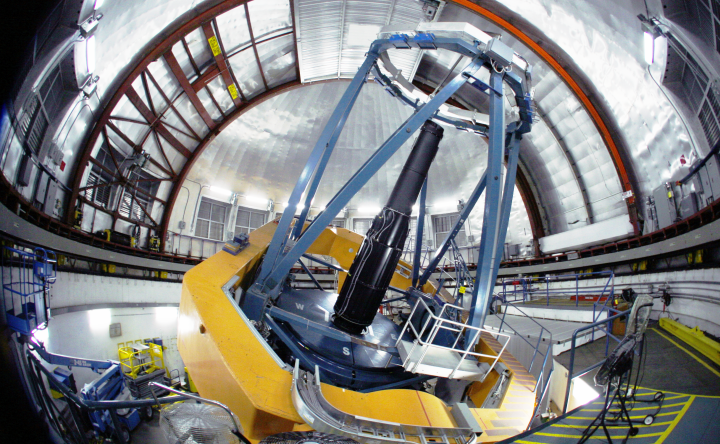
\includegraphics[width=.5\textwidth]{../images/Talk/ukirt_telescope}
			\begin{block}{Near-Infrared}
				\begin{itemize}
					\item In the near-IR our sample was matched to both 2MASS (23,088) and UKIDSS (35,749)
					%\item To increase the number of matches we performer forced photometry on the 2MASS data
				\end{itemize}
			\end{block}}
		\only<4>{
			\centering
			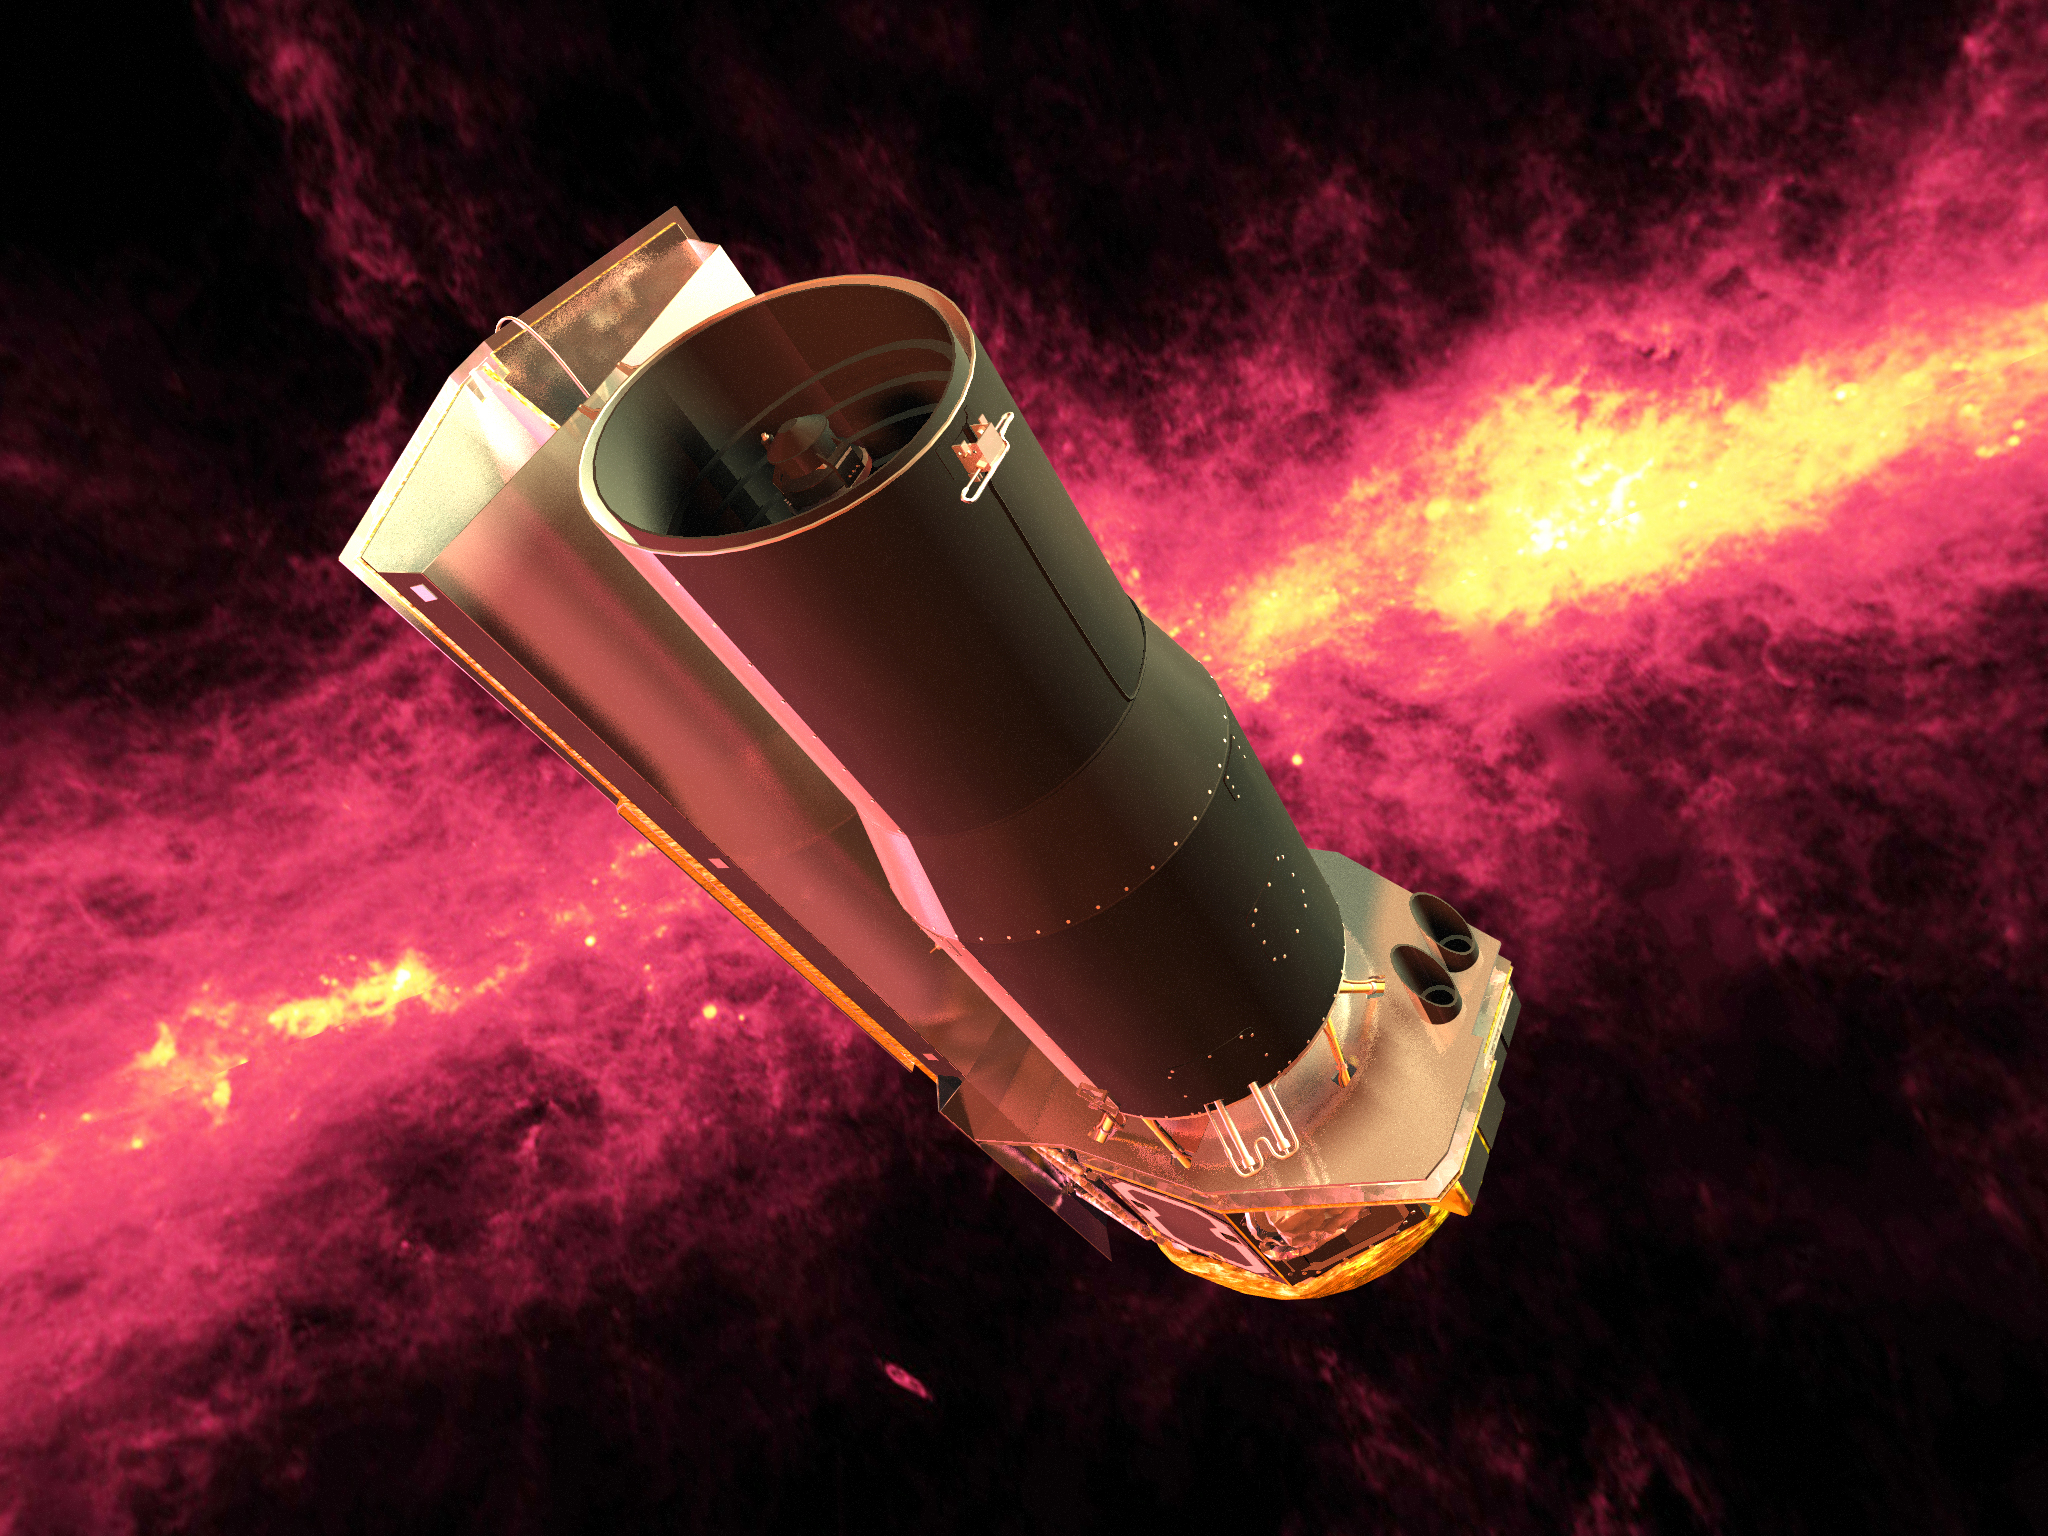
\includegraphics[width=.5\textwidth]{../images/Talk/Spitzer_space_telescope}
			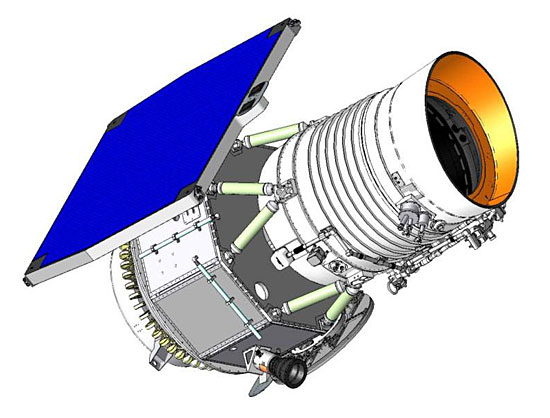
\includegraphics[width=.5\textwidth]{../images/Talk/wise_satellite}
			\begin{block}{Mid-Infrared}
				\begin{itemize}
					\item In the mid-IR our sample was matched to both {\em WISE} (85,358) and {\em Spitzer} (1,196)
				\end{itemize}
			\end{block}}
	\end{column}
	\end{columns}
\end{frame}

\section{Mean SEDs}
\subsection{Full Mean SED}
\begin{frame}
	%\vspace{-2mm}
	\begin{columns}
	\begin{column}{.8\textwidth}
	\begin{center}
		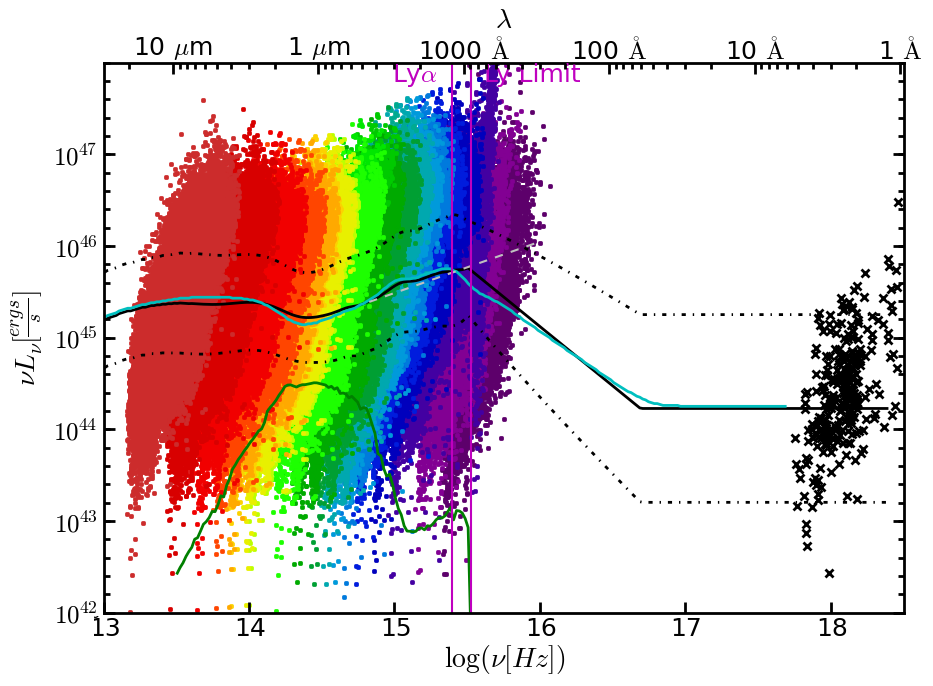
\includegraphics[width=\textwidth]{../images/Talk/f10_crop}
	\end{center}
	\end{column}
	%\vspace{-5mm}
	\begin{column}{.3\textwidth}
	\only<1>{
		\begin{block}{Mean SED}
		\begin{itemize}
			%\item Colored points: photometric data
			\item Black line: New mean SED
			\item Cyan line: \citet{Richards:2006} mean SED
			\item Green line: Typical host galaxy contribution
			\item Black X's: X-ray data
		\end{itemize}
		\end{block}}
	\only<2>{
		\begin{block}{Mean SED}
			``...the large dispersion of shapes in individual objects means that the mean SED should be used only with caution, 
	   		and that the variety of shapes should contain information about the physics of quasars.''
		\end{block}}
	\end{column}
	\end{columns}
\end{frame}

\subsection{Luminosity Dependence of SEDs}
\begin{frame}	
	\begin{columns}
		\begin{column}{0.55\textwidth}
			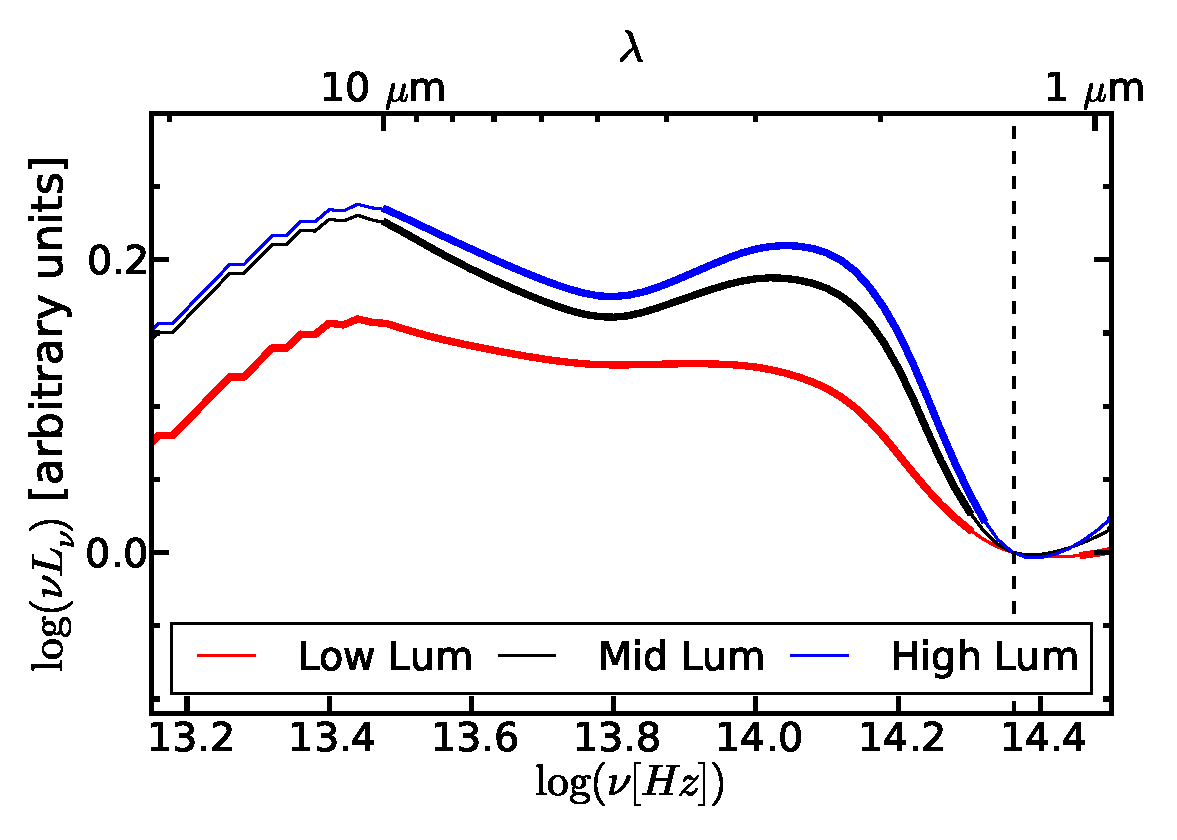
\includegraphics[width=\textwidth]{../images/SEDs/f13a}
		\end{column}
		\begin{column}{0.55\textwidth}
			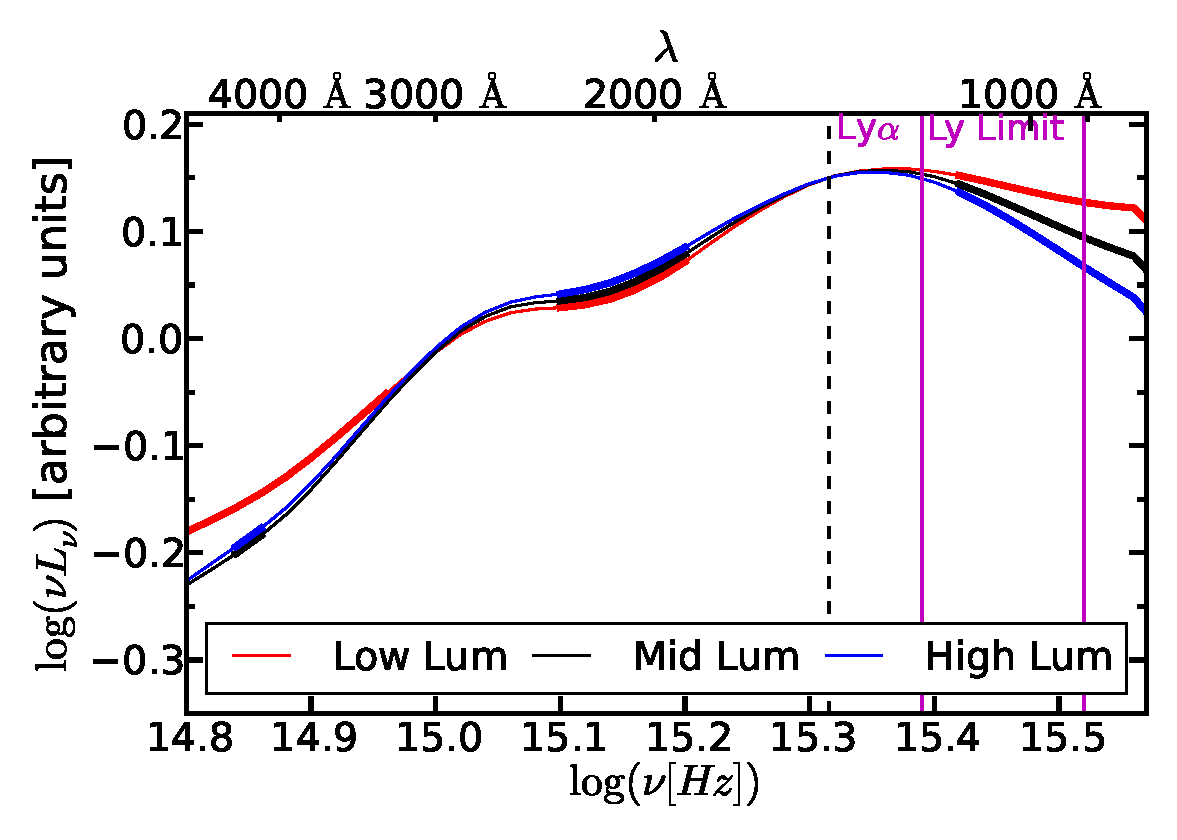
\includegraphics[width=\textwidth]{../images/SEDs/f13b}
		\end{column}
	\end{columns}
	\begin{block}{Luminosity Dependence of SEDs}
		\begin{itemize}
			\item High-luminosity quasars show more hot dust emission in the mid-IR
			\item High-luminosity quasars have a softer (redder) UV continuum
		\end{itemize}
	\end{block}
\end{frame}

\subsection{Eddington Luminosity}
\begin{frame}
	\begin{columns}
	\begin{column}{.2\textwidth}
		\begin{tikzpicture}
			%\draw[help lines,xstep=1,ystep=1] (0,-3) grid (9,3);
			\fill[gray] (1,0) circle (.25);
			\fill[black] (1,-3.5) circle(.5);
			\draw[blue,ultra thick,->] (1,-.255) -- (1,-2.75);
			\draw[red,ultra thick,->] (1,.255) -- (1,2.75);
			\node[anchor=west,inner sep=0] at (1.25,-1.5) {$F_{\rm gravity}$};
			\node[anchor=west,inner sep=0] at (1.25,1.5) {$F_{\rm radiation}$};
			\node[anchor=west,inner sep=0] at (1.5,-3.5) {BH};
		\end{tikzpicture}
	\end{column}
	\begin{column}{.8\textwidth}
		\begin{block}{Eddington Luminosity}
		\begin{itemize}
			\item The luminosity when the outward radiation pressure balances the inward gravitational force
			\begin{itemize}
				\item $L_{\rm Edd} \simeq 1.23 \times 10^{38} \frac{\rm erg}{\rm s} \left( \frac{M_{\rm BH}}{M_{\odot}} \right)$
			\end{itemize}
			\item Assuming a constant accretion rate, the bolometric luminosity can also be written:
			\begin{itemize}
				\item $L_{\rm Bol}=\eta \dot{M} c^2$
			\end{itemize}
			\item Defining $\dot{M}_{\rm Edd}$ as the accretion rate associated with $L_{\rm Edd}$
			\begin{itemize}
				\item $\frac{L_{\rm Bol}}{L_{\rm Edd}} = \frac{\dot{M}}{\dot{M}_{\rm Edd}}$
			\end{itemize}
		\end{itemize}
		\end{block}
	\end{column}
	\end{columns}
\end{frame}

\subsection{BC Dependence of SEDs}
\begin{frame}
	\begin{columns}
	\begin{column}{.75\textwidth}
		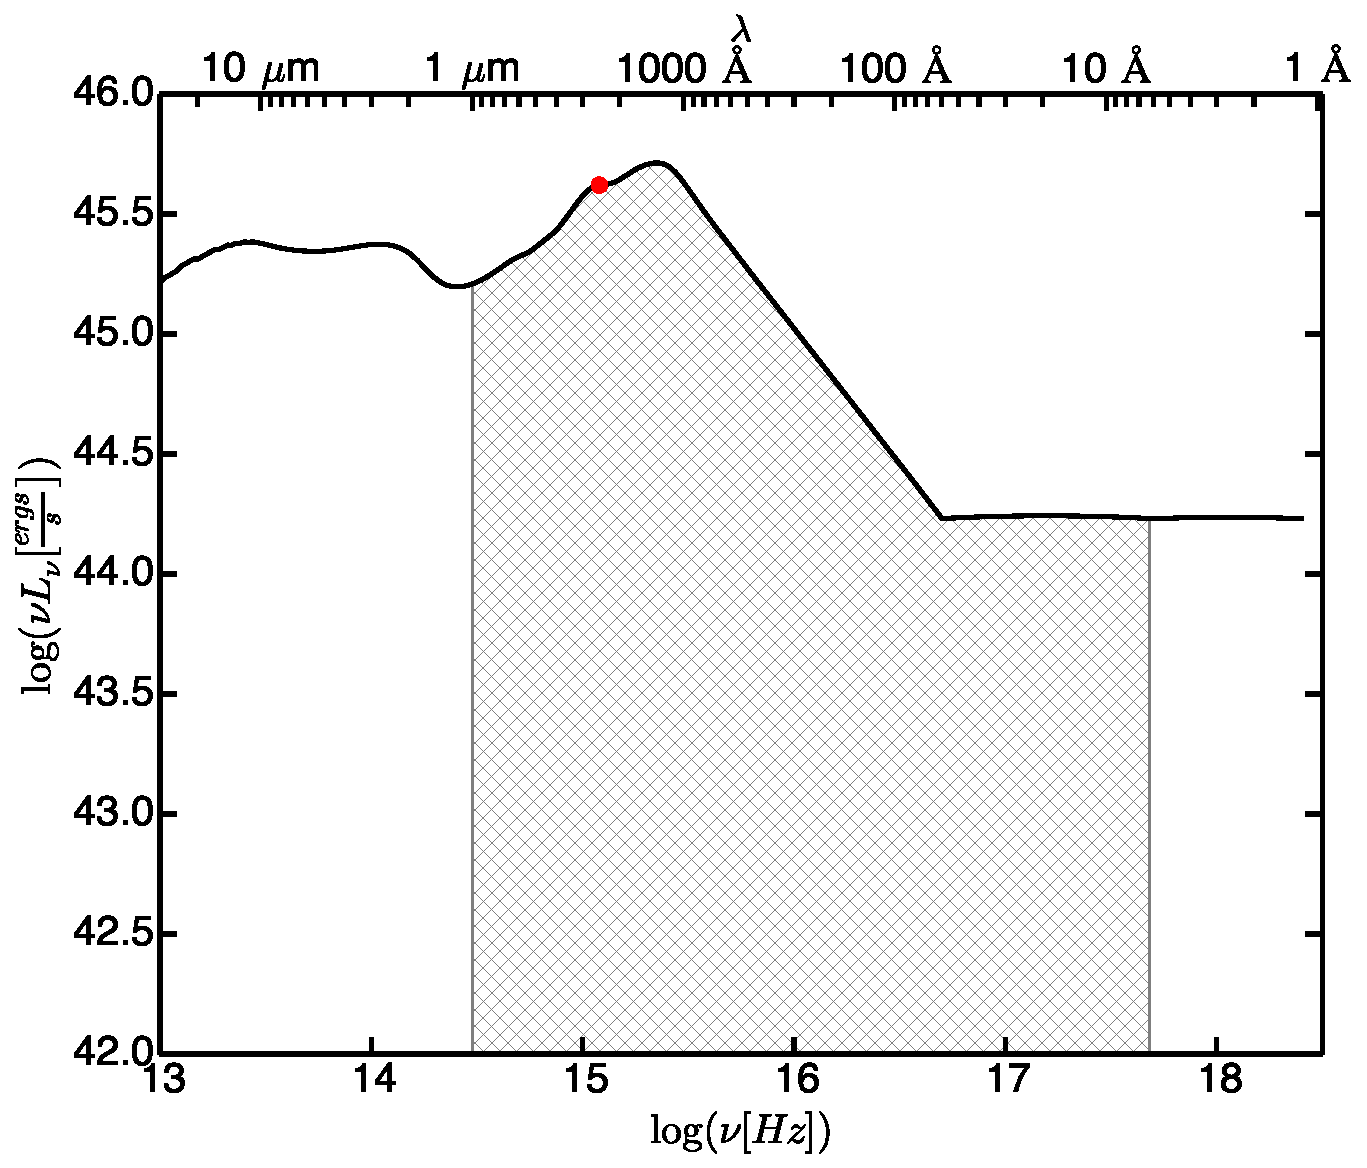
\includegraphics[width=\textwidth]{../images/Talk/BC}
	\end{column}
	\begin{column}{.35\textwidth}
		\centering
		\begin{block}{BCs}
		\begin{itemize}
			%\item The bolometric luminosity of a quasar is related to the accretion rate of the central black hole
			\item The bolometric luminosity can only be measured if you have a full multi-wavelength SED
			\item When this is not the case a bolometric correction (BC) is used to convert a mono-chromatic luminosity into a bolometric one
		\end{itemize}
		\end{block}
		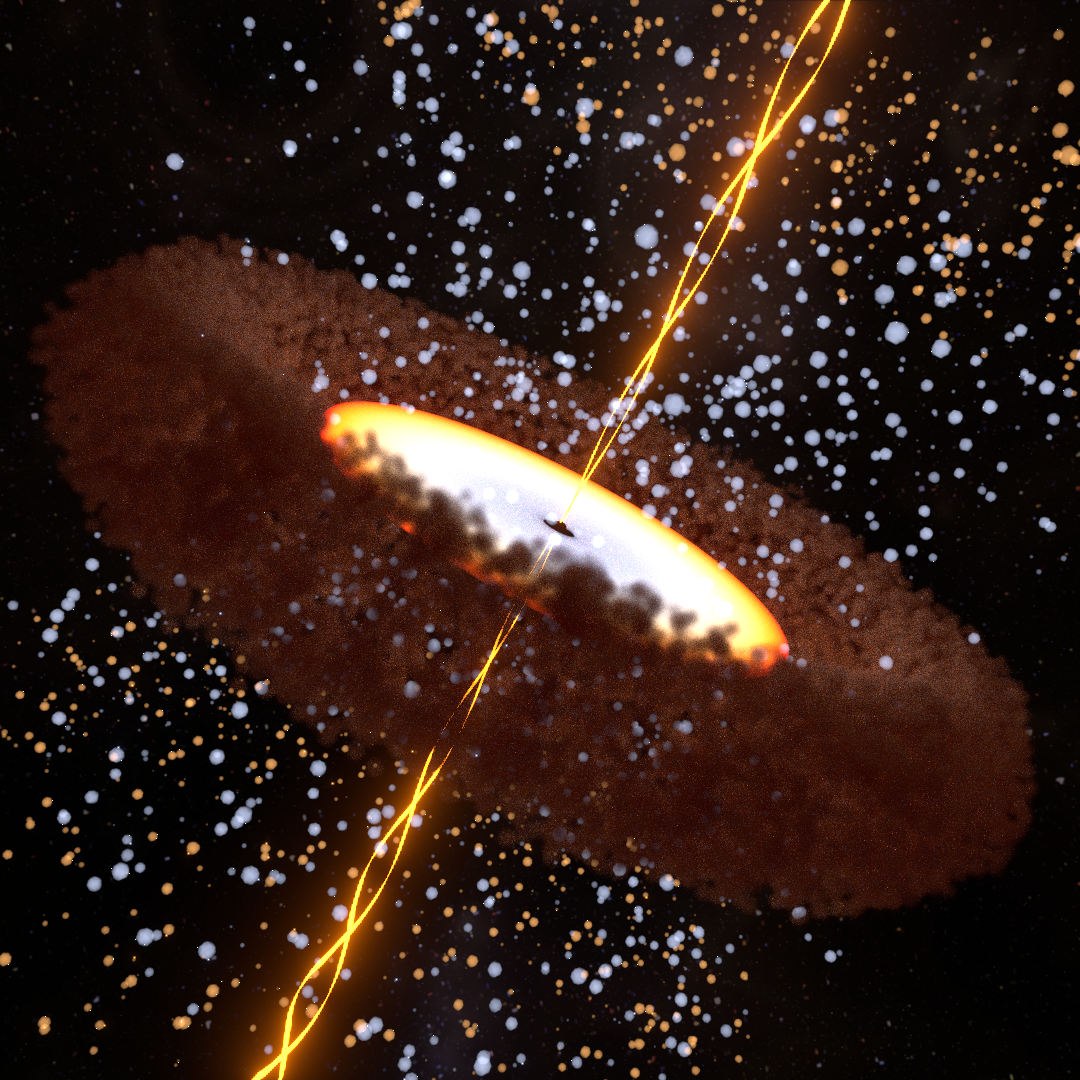
\includegraphics[width=.5\textwidth]{../images/Talk/agn_03}
	\end{column}
	\end{columns}
\end{frame}

\begin{frame}
	\begin{center}
		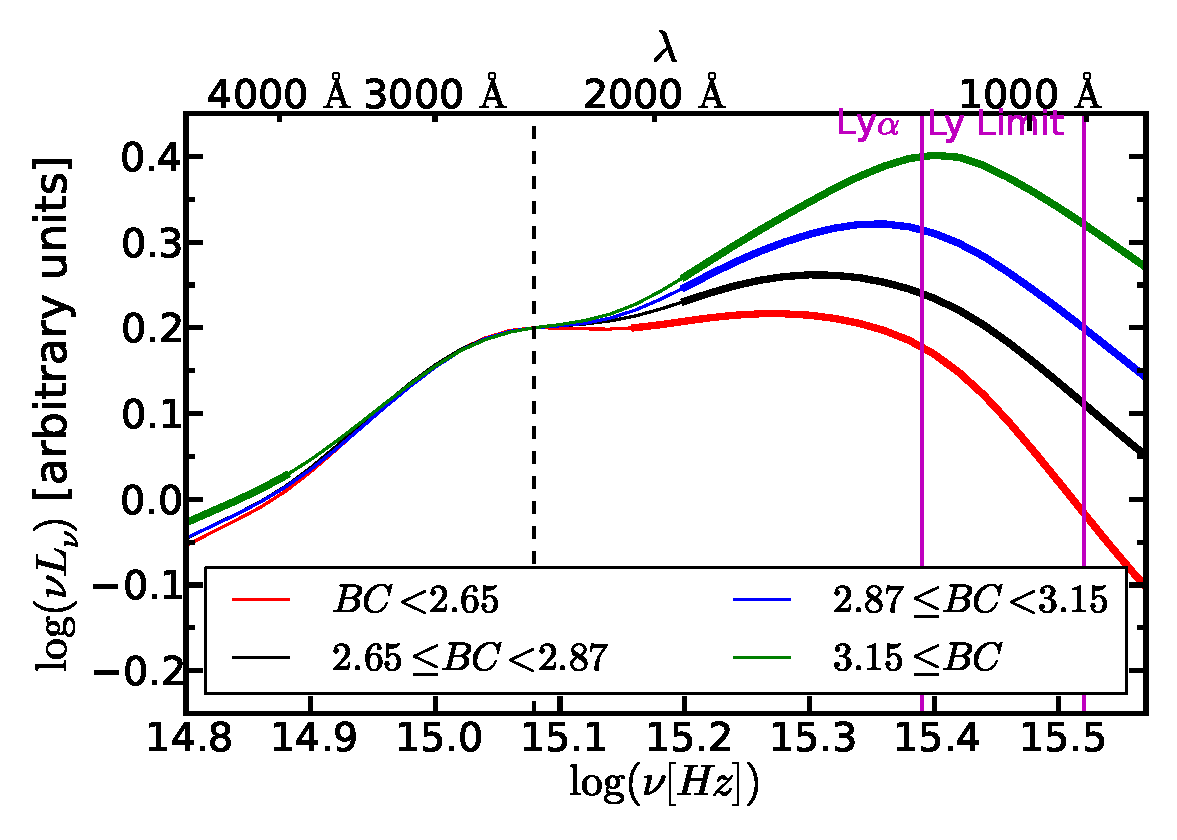
\includegraphics[width=0.78\textwidth]{../images/SEDs/f13d}
	\end{center}
	\vspace{-.4cm}
	\begin{block}{Bolometric Correction Dependence of SEDs}
		\begin{itemize}
			\item BC is the multiplication factor needed to turn $L_{2500\textup{\AA}}$ into $L_{bol}$
			\item The range of BCs come from differences in the UV continua
		\end{itemize}
	\end{block}
\end{frame}

\subsection{The Unseen EUV}
\begin{frame}
	\begin{columns}
		\begin{column}{0.6\textwidth}
			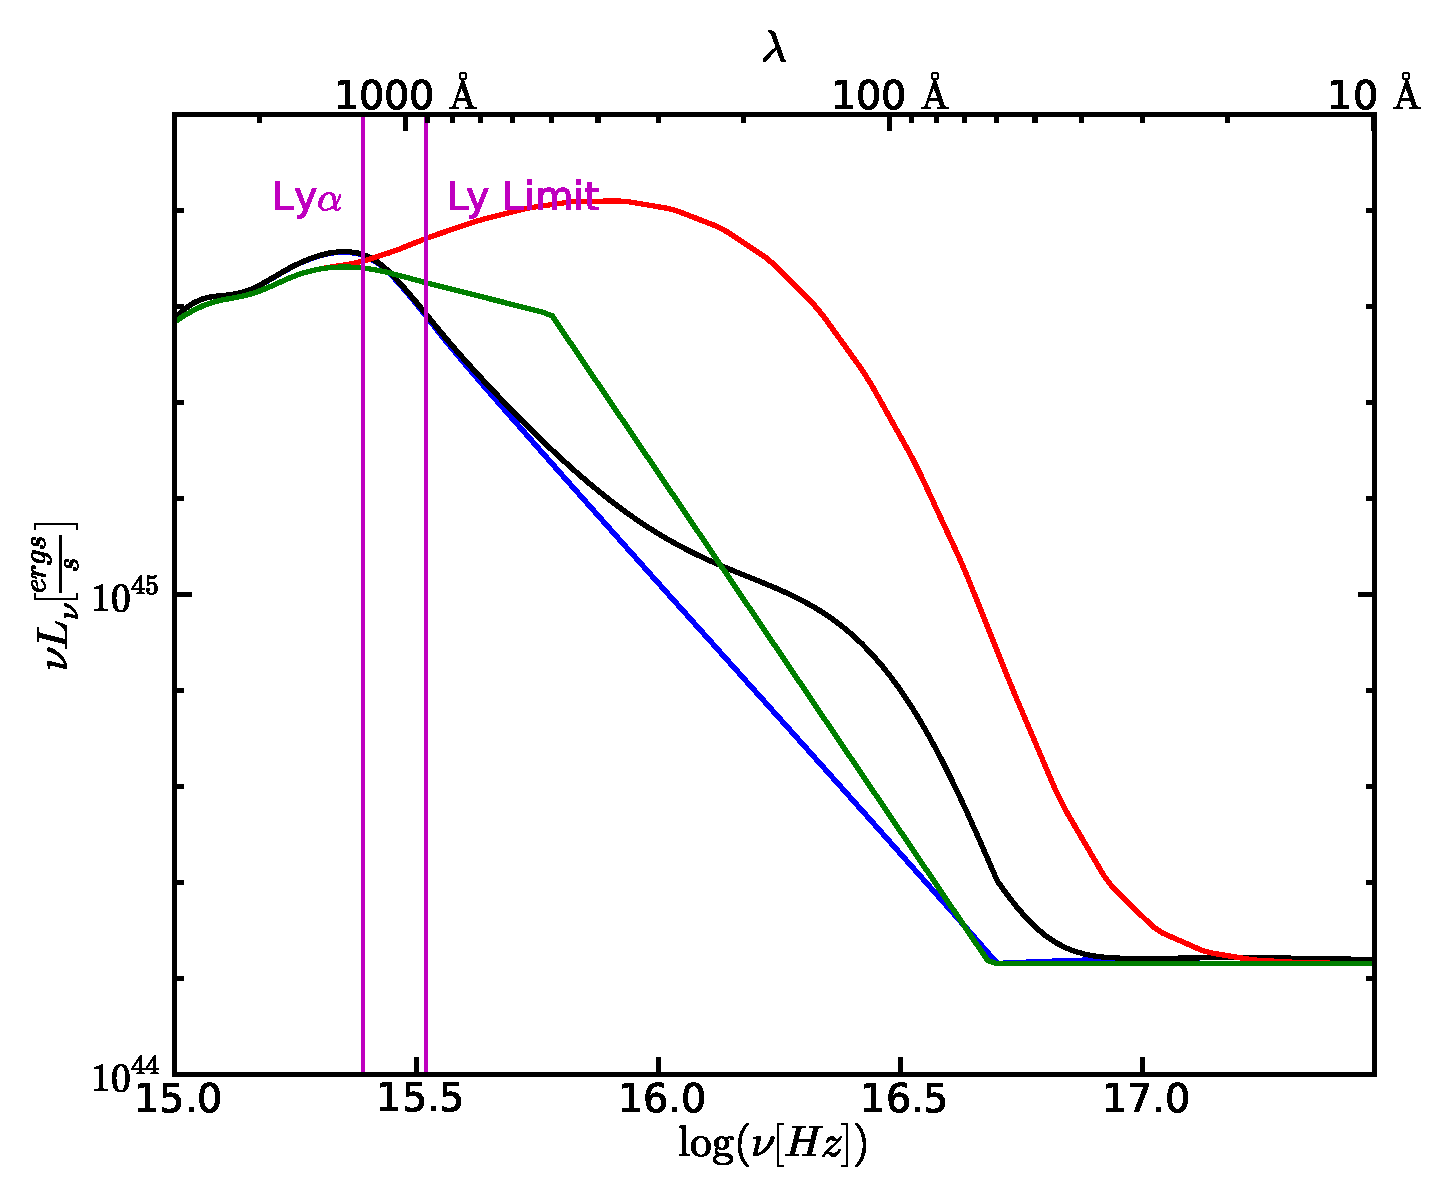
\includegraphics[width=\textwidth]{../images/SEDs/f18a}
		\end{column}
		\begin{column}{0.6\textwidth}
			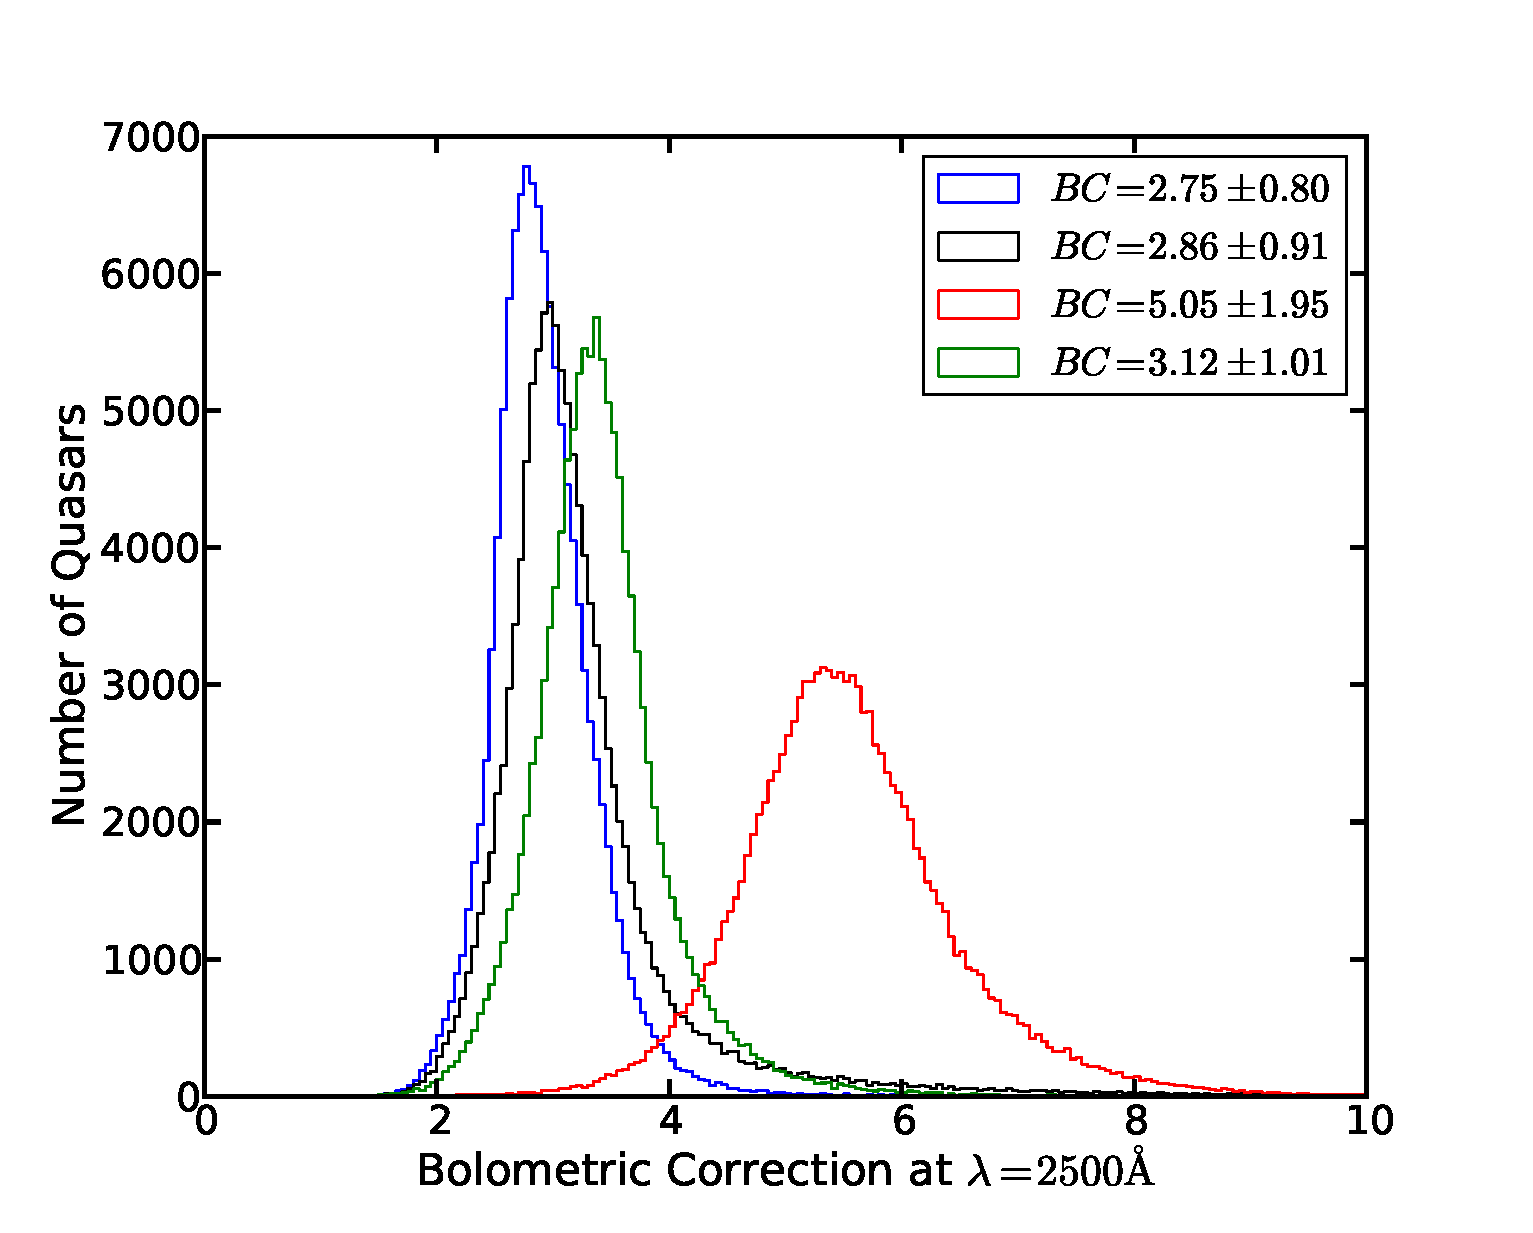
\includegraphics[width=\textwidth]{../images/SEDs/f18b}
		\end{column}
	\end{columns}
	\vspace{-2mm}
	\begin{block}{Various models for the extreme-UV and the resulting BCs}
		\begin{itemize}
			\item Blue: Powerlaw
			\item Black: Fixed luminosity blackbody
			\item Red: Theory based \citep[from CLOUDY;][]{Casebeer:2006}
			\item Green: Data based \citep{Scott:2004}					
		\end{itemize}
	\end{block}
	\end{frame}

\section{Dusty Quasars}
\subsection{Red vs. Reddened}
\begin{frame}
	\setbeamercovered{transparent}
	\centering
	\begin{tikzpicture}
		\node[anchor=south west,inner sep=0] (image) at (1.5,0) {
			%\begin{centering}
			\includegraphics<4>[width=\textwidth]{../images/Dust/f3}
			%\end{centering}
			};		
		%\draw<2>[help lines,xstep=1,ystep=1] (0,0) grid (11,4);
		\draw<1-3>[thick,->] (1.5,.5) -- (5,.5) node[anchor=north] {$\lambda$};
		\draw<1-3>[thick,->] (1.5,.5) -- (1.5,3.5) node[anchor=east] {$L$};
		\draw<1-3>[thick,blue] (4,1) -- (2,3);
		\draw<1-3>[thick,red] (4,1) -- (2,2);
		\node<1-3>[anchor=south west,inner sep=0,blue] at (1.5,0) {Blue};
		\node<1-3>[anchor=south west,inner sep=0,red] at (4,0) {Red};
		\draw<1>[thick,white,->] (6,.5) -- (9.5,.5) node[anchor=north] {$\lambda$};
		\draw<3>[thick,dashed] (2.25,.5) --(2.25,3.5);
		\draw<3>[thick,dashed] (2.5,.5) --(2.5,3.5);
		\draw<3>[thick,dashed] (3.25,.5) --(3.25,3.5);
		\draw<3>[thick,dashed] (3.5,.5) --(3.5,3.5);
		
		\draw<2-3>[thick,->] (6,.5) -- (9.5,.5) node[anchor=north] {$\lambda$};
		\draw<2-3>[thick,->] (6,.5) -- (6,3.5) node[anchor=east] {$L$};
		\draw<2-3>[thick,blue] (8.5,1) -- (6.5,3);
		\draw<2-3>[thick,red] (8.5,1) .. controls (7.5,1.9) .. (6.5,2);
		\node<2-3>[anchor=south west,inner sep=0,blue] at (6,0) {Blue};
		\node<2-3>[anchor=south west,inner sep=0,red] at (8.5,0) {Red};
		\draw<3>[thick,dashed] (6.75,.5) --(6.75,3.5);
		\draw<3>[thick,dashed] (7,.5) --(7,3.5);
		\draw<3>[thick,dashed] (7.75,.5) --(7.75,3.5);
		\draw<3>[thick,dashed] (8,.5) --(8,3.5);
	\end{tikzpicture}
	\only<4>{\vspace{-3mm}}
	\only<1-3>{\vspace{1.25mm}}
	\begin{block}{Red vs. Reddened}
		\only<1-3>{
		\begin{itemize}
			\item<1-3> Quasars that are intrinsically red follow a powerlaw in the optical--UV
			\item<2-3> Quasars that are dust reddened have shorter wavelength absorbed by dust adding curvature to the optical--UV
			\item<3> Color is the slope between each set of dashed lines
		\end{itemize}
		}
		\only<4>{
		\begin{itemize}
			\item Dust reddening causes the colors at shorter wavelengths (left) to have a heavier red tail than the colors at longer wavelengths (right)
		\end{itemize}
		}
	\end{block}
\end{frame}

\subsection{Extinction Laws}
\begin{frame}
	\begin{columns}
		\begin{column}{0.35\textwidth}
			\begin{block}{Extinction Laws}
				\begin{itemize}
					\item In order to study properties that are associated with the physics of a quasar we need to find the {\em intrinsic} SED
					\item Extinction laws characterize how much light various types of dust absorb at a given wavelength
					\item The strength of dust extinction is measured using the color excess E(B-V)
					%\item{Dust extinction: combination of scatting and absorption}
					%\item{$A_X$: extinction in the $X$ filter}
					%\item{E$(X-Y) = A_X - A_Y$: color excess in $X-Y$}
					%\item{$R_{\lambda} = \frac{A_{\lambda}}{\rm E(B-V)}$: dust reddening law}
					%\item{$R_{V}$ is typically used to parametrize the reddening curves}
					%\item{Larger values of $R_{V}$ correspond to larger dust grains}				
				\end{itemize}
			\end{block}
		\end{column}
		\begin{column}{0.65\textwidth}
			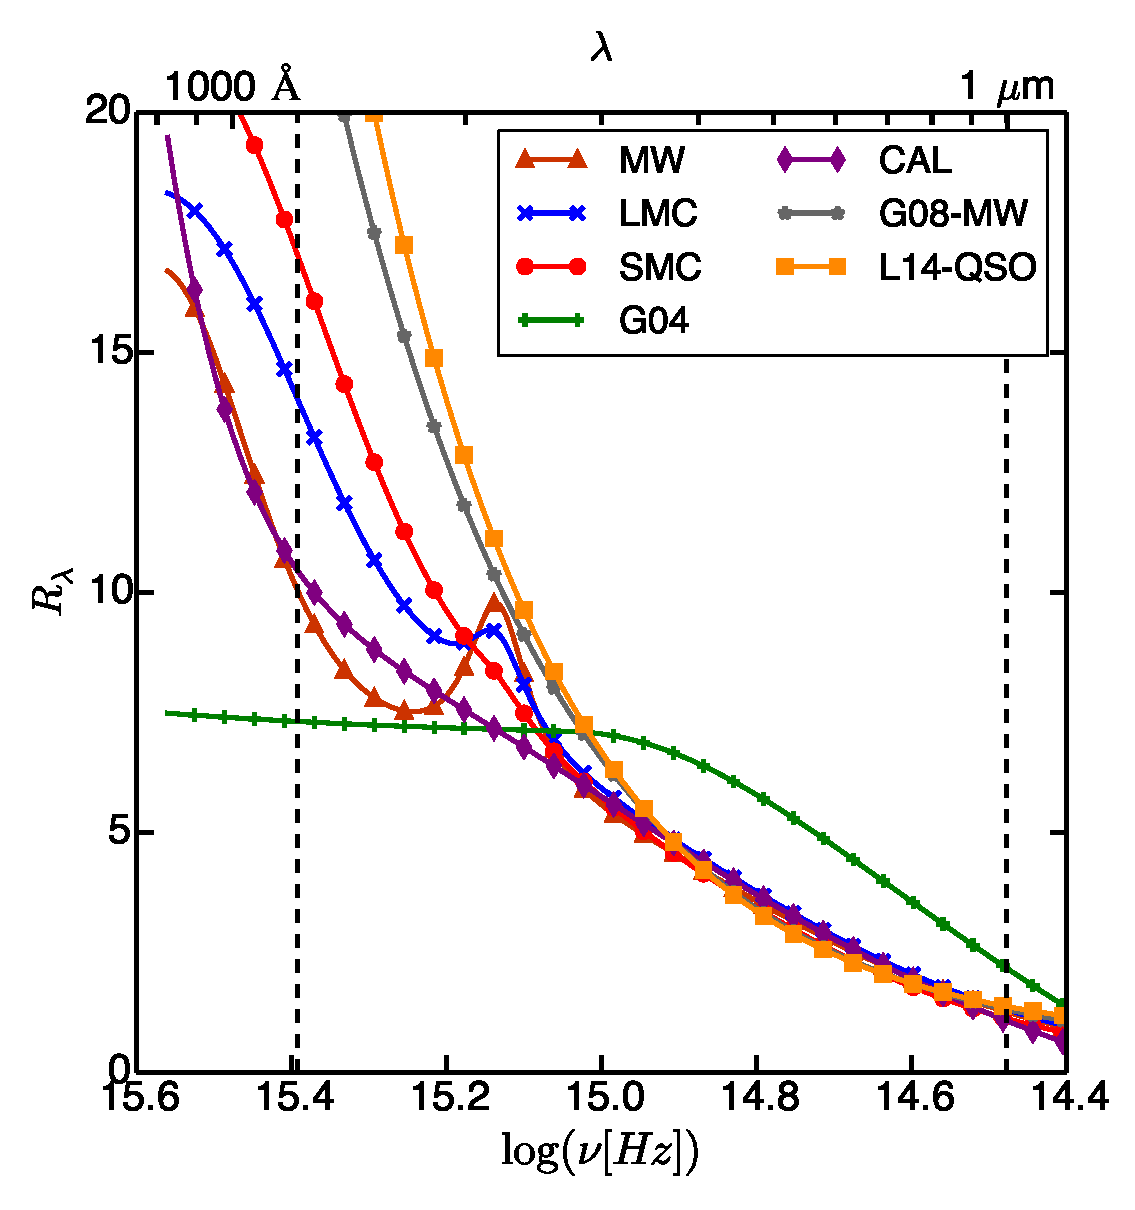
\includegraphics[width=\textwidth]{../images/Dust/f4}
		\end{column}
	\end{columns}
\end{frame}


%\begin{frame}
%	\vspace{1mm}
%	\begin{tikzpicture}
%		\node[anchor=south west,inner sep=0] (image) at (0,0) {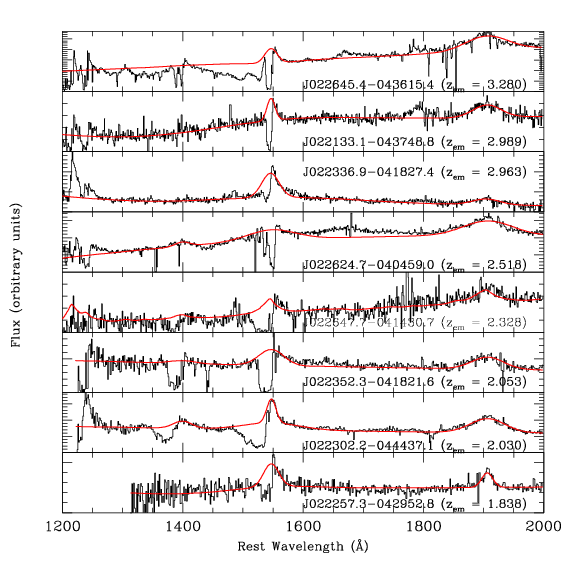
\includegraphics[trim={1cm 10.6cm 0 3.2cm},clip,width=\textwidth]{../images/Talk/BAL_spec}};
%		\begin{scope}[x={(image.south east)},y={(image.north west)}]
%			\node at (.95,-.05) {\tiny \citet{Stalin:2011}};
%		\end{scope}
%	\end{tikzpicture}
%	\vspace{-8mm}
%	\begin{block}{BAL quasars}
%	\begin{itemize}
%		\item Some quasars show broad absorption lines (BAL) at the same redshift as the quasar
%		\item These BALs are caused by an outflow of gas from the quasar
%		\item BAL quasars have been found to have different dust extinction properties than non-BAL quasars
%	\end{itemize}
%	\end{block}
%\end{frame}

\begin{frame}
	\setbeamercovered{transparent}
	\makebox[\textwidth][c]{
	\includegraphics<1>[width=1.1\textwidth]{../images/Talk/f5b}
	\includegraphics<2>[width=1.1\textwidth]{../images/Talk/f5}
	}
	\begin{block}{$c_1$ vs. $c_2$}
	\begin{itemize}
		\item<1-> We can determine the extinction law to use by looking at the slopes and curvatures of the SEDs
		\item<2> The quasars seem to follow the steeper reddening laws: Small Magellanic Cloud (SMC) and/or multiple scattering \citep{Goobar:2008} laws
	\end{itemize}
	\end{block}
\end{frame}

\subsection{Fitting the data}
\begin{frame}
	\begin{block}{Goal}
		\begin{itemize}
			\item{Fit for {\em individual} values for both the powerlaw index w.r.t. the mode, $\Delta(\alpha_\lambda)$, and the reddening amount, E(B-V)}
			\item{Break the degeneracy between these values}
			\item{Fit for the {\em ensemble} distributions for $\Delta(\alpha_\lambda)$ and E(B-V)}
		\end{itemize}
	\end{block}
	\begin{block}{Method}
		\begin{itemize}
			\item{Hierarchical Bayesian model}
				\begin{itemize}
					\item{Assume functional form for the ensemble distributions}
					\item{Fits for both the individual values {\em and} the shapes of the ensemble distributions at the same time}
					\item{This allows errors to be propagated across all levels of the model}
				\end{itemize}
		\end{itemize}
	\end{block}	
\end{frame}

\begin{frame}[label=SMC_fits]
	\begin{columns}
		\begin{column}{0.52\textwidth}
			\begin{tikzpicture}
				\node[anchor=south west,inner sep=0] (image) at (0,0) {\includegraphics<1->[width=\textwidth]{../images/Talk/f10a}};
				\begin{scope}[x={(image.south east)},y={(image.north west)}]
					\node<1->[anchor=south west,inner sep=0,red] at (.1,0) {Red};
					\node<1->[anchor=south west,inner sep=0,blue] at (.65,0) {Blue};
					\node<1->[anchor=north west,inner sep=0,red,rotate=90] at (0,.65) {Dust};
					\node<1->[anchor=north west,inner sep=0,blue,rotate=90] at (0,.1) {No Dust};
					\draw<2>[red,ultra thick] (.6,.4) circle (.1);
					\draw<2>[red,ultra thick] (.12,.18) -- (.78,.18);
					\draw<2>[red,ultra thick] (.41,.07) -- (.41,.77);
				\end{scope}
			\end{tikzpicture}
		\end{column}
		\begin{column}{0.52\textwidth}
			\begin{tikzpicture}
				\node[anchor=south west,inner sep=0] (image) at (0,0) {\includegraphics<1->[width=\textwidth]{../images/Talk/f10b}};
				\begin{scope}[x={(image.south east)},y={(image.north west)}]
					\node<1->[anchor=south west,inner sep=0,red] at (.1,0) {Red};
					\node<1->[anchor=south west,inner sep=0,blue] at (.65,0) {Blue};
					\node<1->[anchor=north west,inner sep=0,red,rotate=90] at (0,.65) {Dust};
					\node<1->[anchor=north west,inner sep=0,blue,rotate=90] at (0,.1) {No Dust};
					\draw<2>[red,ultra thick] (.6,.4) circle (.1);
					\draw<2>[red,ultra thick] (.12,.18) -- (.78,.18);
					\draw<2>[red,ultra thick] (.41,.07) -- (.41,.77);
				\end{scope}
			\end{tikzpicture}
		\end{column}
	\end{columns}
	\begin{block}{SMC fit}
		\begin{itemize}
			\item The BAL sample has more dust reddening% than the non-BAL sample
			\item The heavily reddened BAL quasars are bluer than heavily reddened non-BAL quasars
		\end{itemize}
	\end{block}
\end{frame}

\subsection{Stacked spectra}
\begin{frame}
	\setbeamercovered{transparent}
	\begin{columns}
		\begin{column}{0.35\textwidth}
		\only<1>{
			\begin{block}{SMC non-BAL}
			\begin{itemize}
				\item Black: typical powerlaw in bin
				\item Red: modal powerlaw
				\item Colors: amount of reddening
				\item Dashed: fit based on photometry
				\item The fits based on the photometry track the spectra well
			\end{itemize}
			\end{block}}
		\only<2->{
			\begin{block}{SMC non-BAL}
			\begin{itemize}
				\item<2> The most reddened spectra in each bin require a steeper reddening law
				\item<3> The least reddened blue spectra starts to turn over faster (i.e. has a softer SED in the EUV)
			\end{itemize}
			\end{block}}
		\end{column}
		\begin{column}{0.72\textwidth}
			\begin{tikzpicture}
				\node[anchor=south west,inner sep=0] (image) at (0,0) {
				\includegraphics<1>[width=\textwidth]{../images/Talk/f12}
				\includegraphics<2>[trim={1cm 21.5cm 18.5cm 0},clip,width=\textwidth]{../images/Talk/f12}
				\includegraphics<3>[trim={20.3cm 4cm 0 17.1cm},clip,width=\textwidth]{../images/Talk/f12}
				};
				\begin{scope}[x={(image.south east)},y={(image.north west)}]
					%\draw<2->[help lines,xstep=.1,ystep=.1] (0,0) grid (1,1);
					\draw<2>[red,ultra thick] (.55,.2) ellipse (.4 and .17);
					\draw<3>[red,ultra thick] (.1,.76) ellipse (.1 and .08);
				\end{scope}
			\end{tikzpicture}
		\end{column}
	\end{columns}
\end{frame}


\begin{frame}
	\setbeamercovered{transparent}
	\begin{columns}
		\begin{column}{0.35\textwidth}
			\begin{block}{non-BAL Spectral Lines}
			\begin{itemize}
				\item<1> The trends seen in \ion{He}{2}, \ion{C}{3}], and \ion{Al}{3} indicate the bluer quasars have softer (redder) EUV spectra
				\item<2> The H$\beta$ line indicates that the bluer quasars could be seen closer to edge-on and/or have larger central black hole masses
			\end{itemize}
			\end{block}
		\end{column}
		\begin{column}{0.75\textwidth}
			\centering
			\includegraphics<1->[width=.8\textwidth]{../images/BH/alpha_colorbar}\\
			\includegraphics<1>[trim={10cm 22cm 9.25cm 0},clip,width=\textwidth]{../images/Dust/f14}
			\only<2>{
				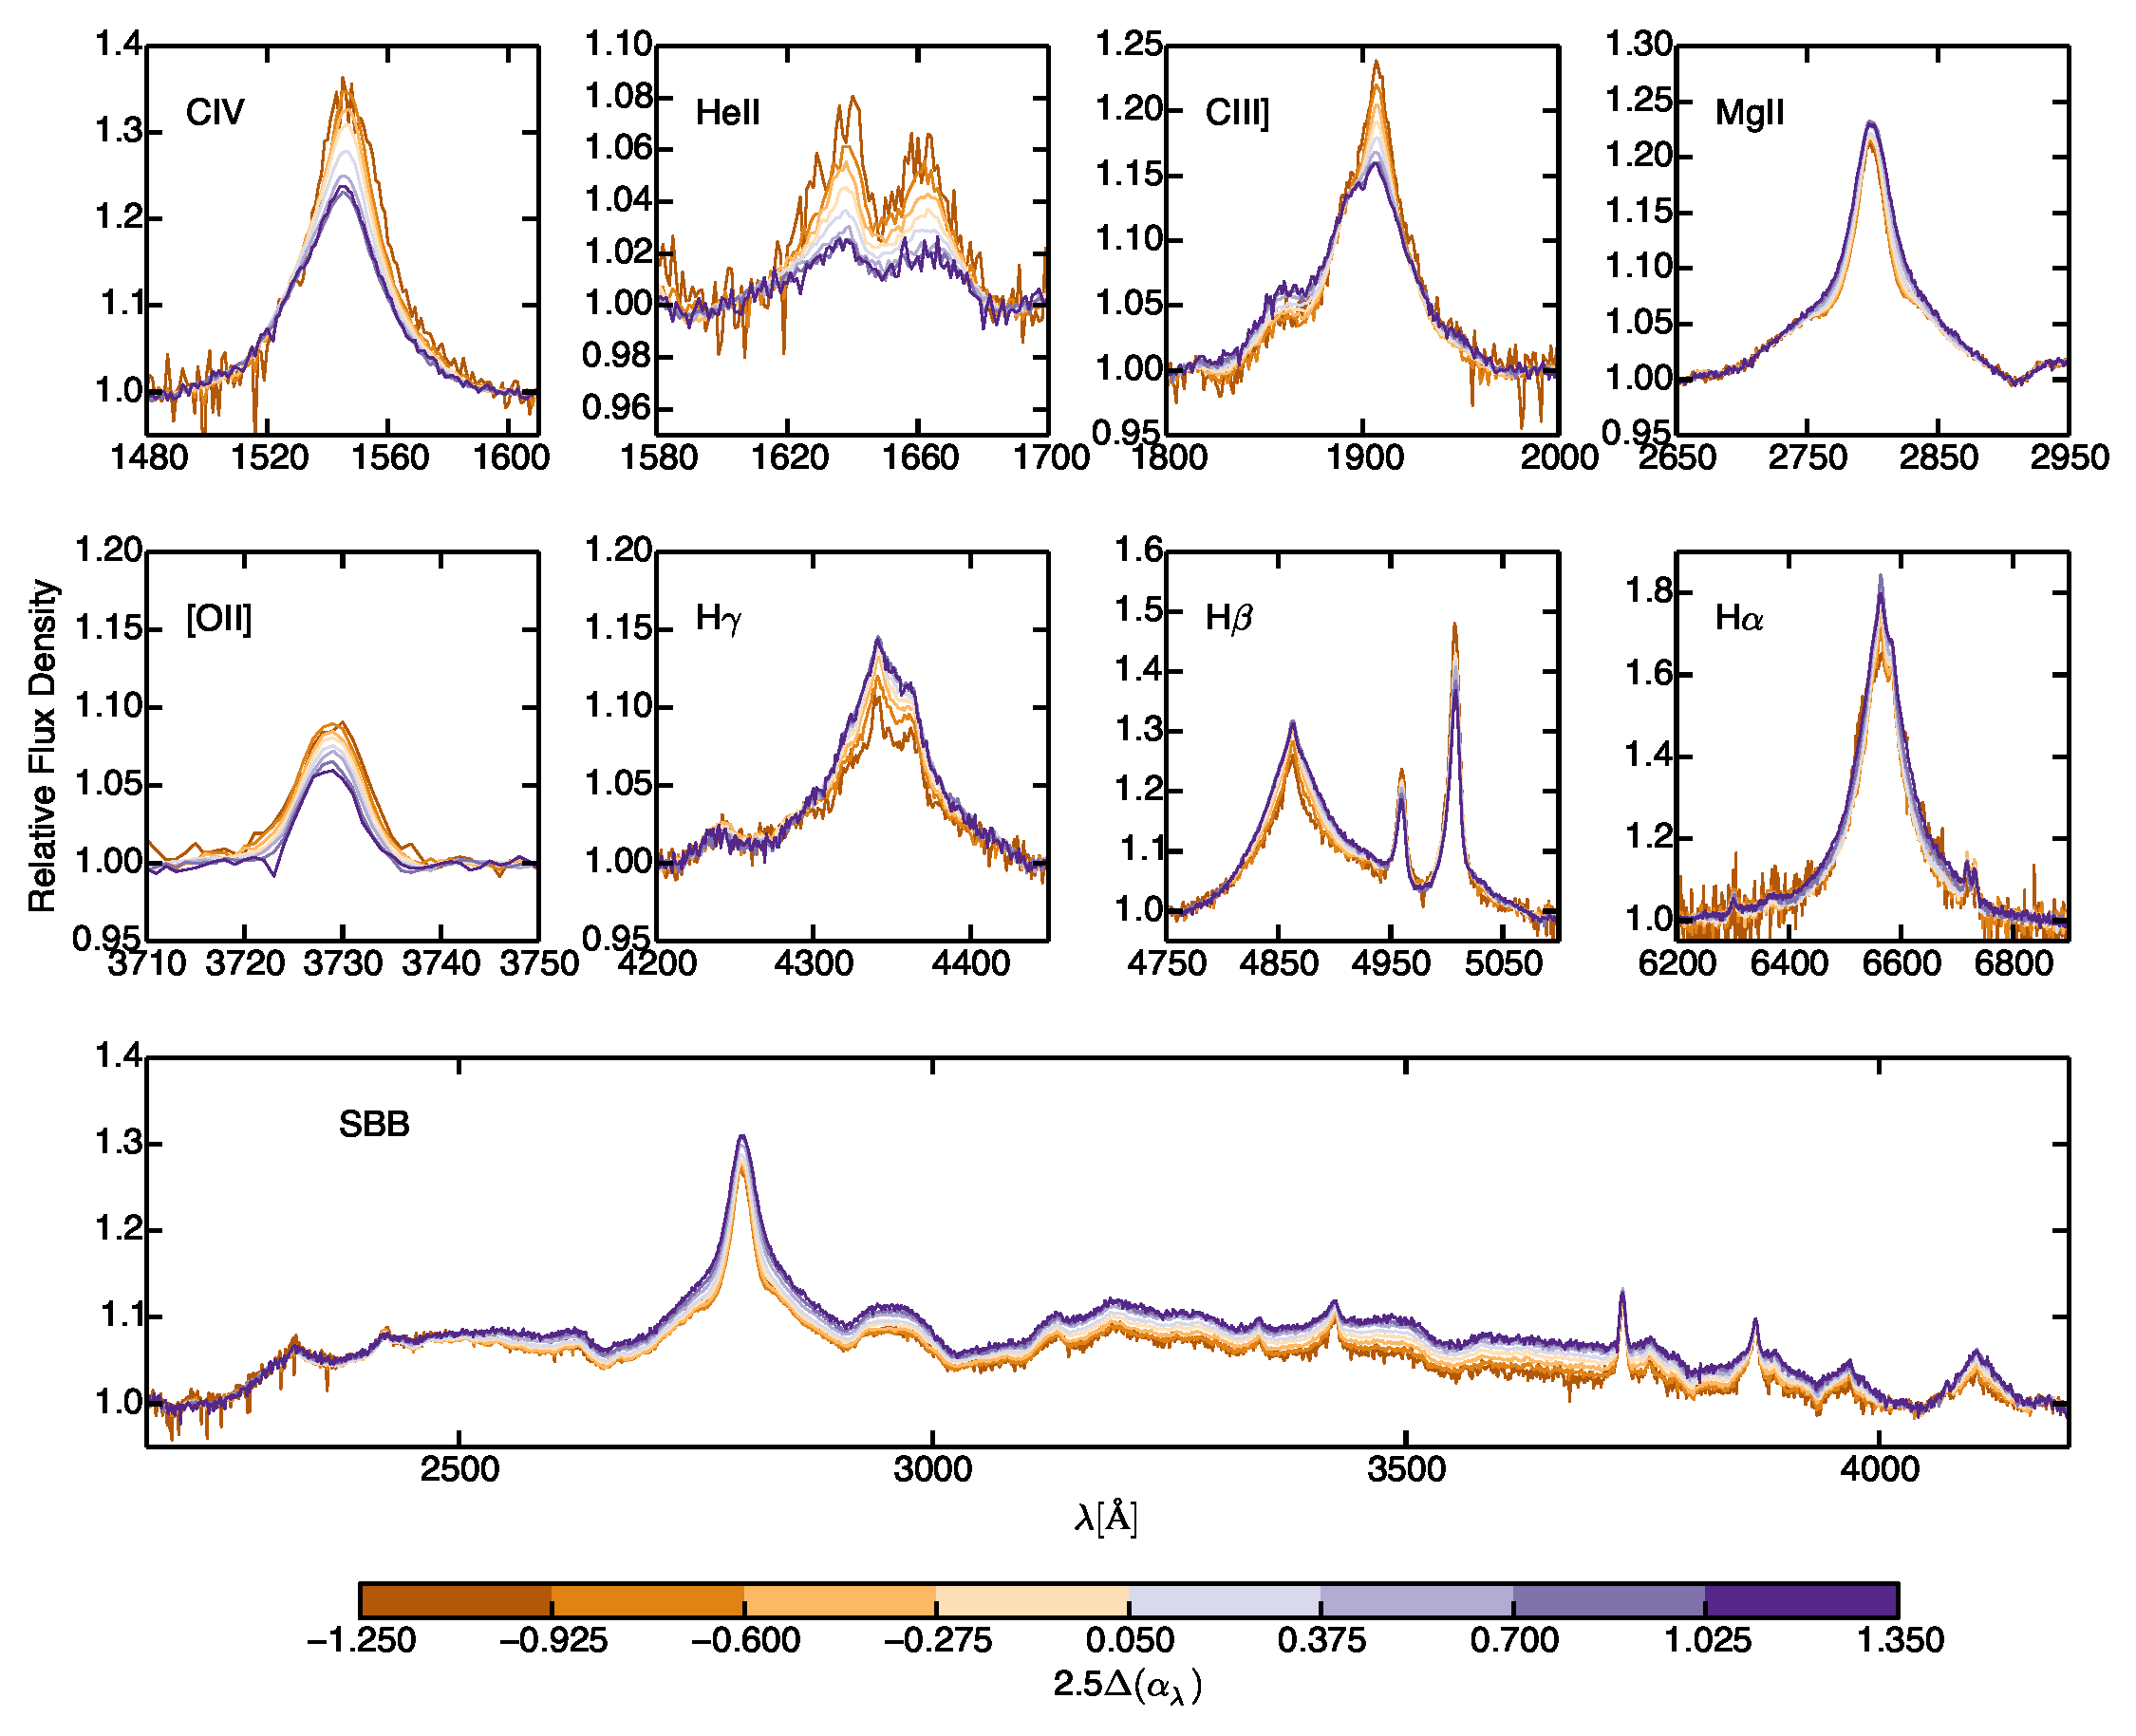
\includegraphics[trim={19.05cm 12cm 9.2cm 9cm},clip,width=.4\textwidth]{../images/Dust/f14}\\
				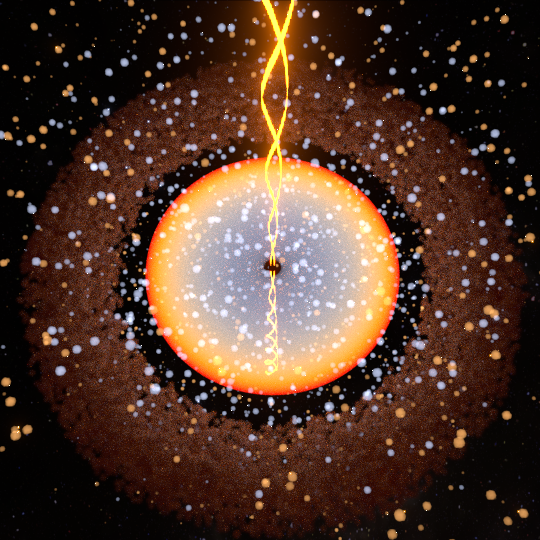
\includegraphics[width=.3\textwidth]{../images/Talk/agn_face_on} \hspace{1cm}
				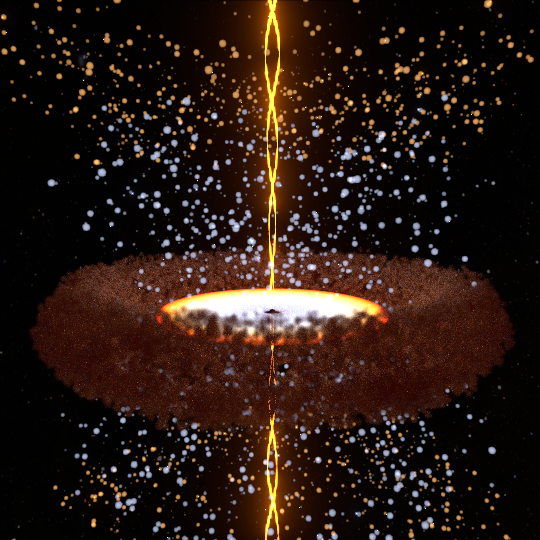
\includegraphics[width=.3\textwidth]{../images/Talk/agn_edge_on}}
		\end{column}
	\end{columns}
\end{frame}

\subsection{Mean SEDs}
\begin{frame}
	\setbeamercovered{transparent}
	\begin{columns}
		\begin{column}{.35\textwidth}
			\begin{block}{E(B-V) dependent SEDs}
			\begin{itemize}
				\item<1-> With more physical variables defined we look for trends in the mean SEDs
				\item<1-> Some sample selection and/or intrinsic effect is a function of E(B-V)
				\item<2> More reddened quasars have less hot dust emission
				\item<3> More reddened quasars have a redder spectral index from 5--11$\mu$m
			\end{itemize}
			\end{block}
		\end{column}
		\begin{column}{.75\textwidth}
			\begin{tikzpicture}
				\node[anchor=south west,inner sep=0] (image) at (0,0) {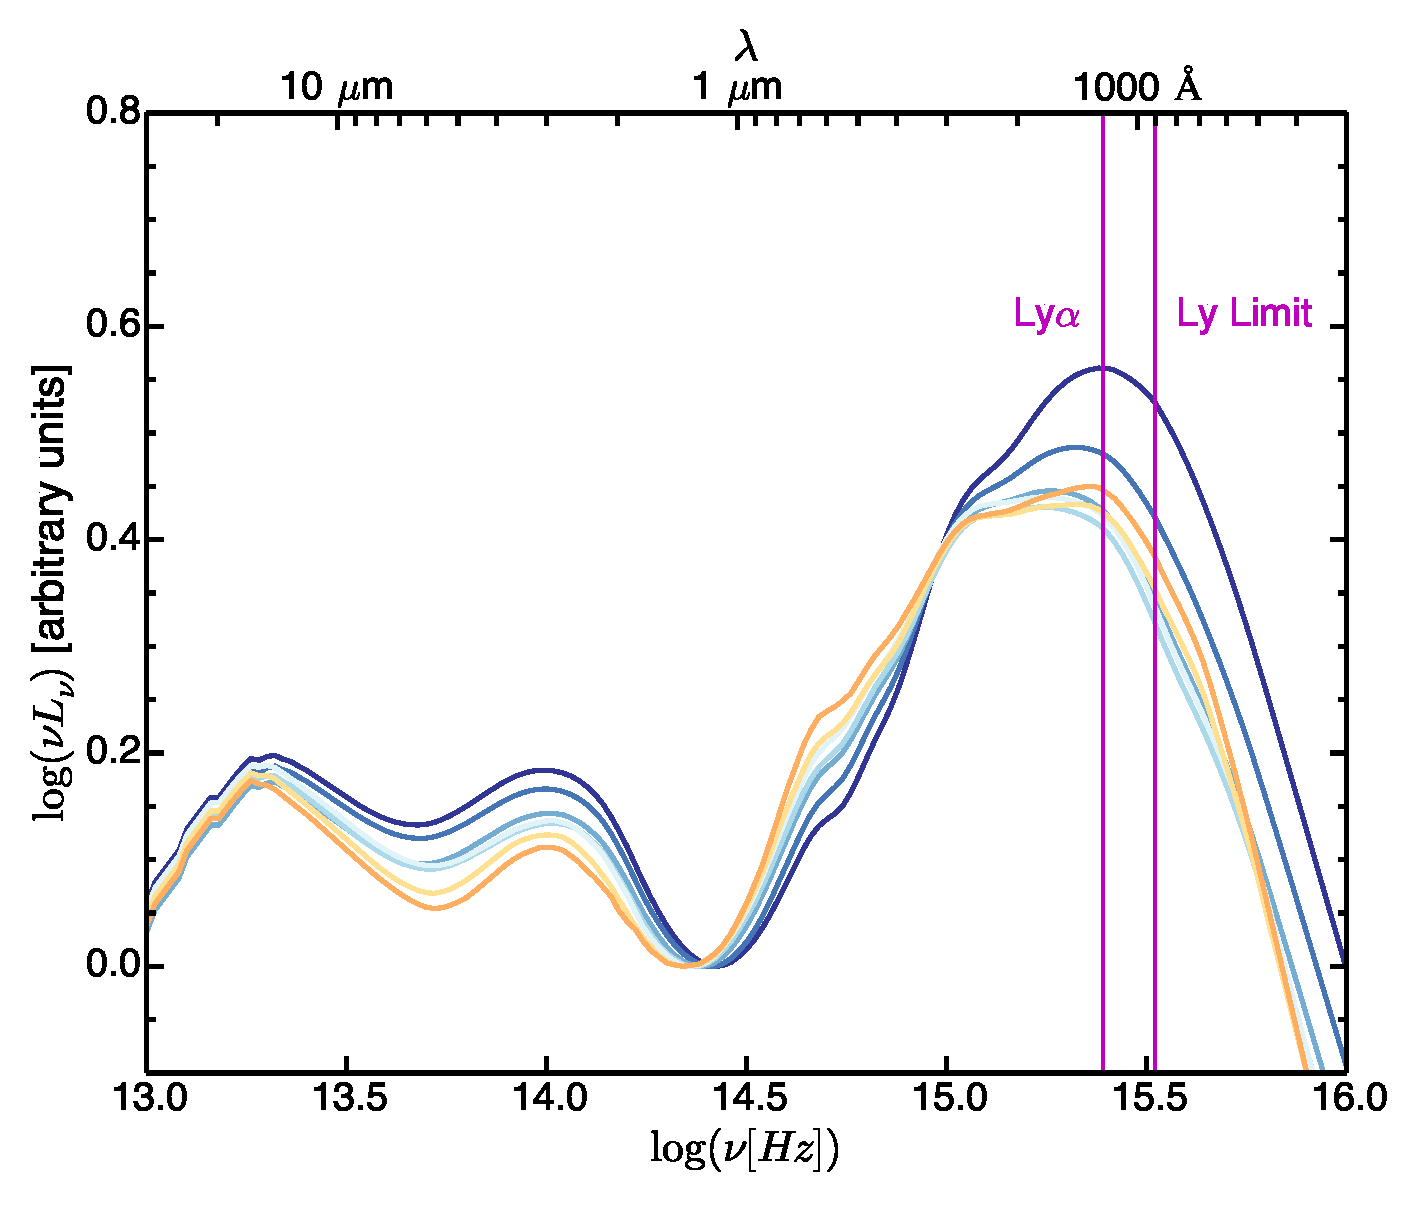
\includegraphics[width=\textwidth]{../images/BH/f4a}};
				\begin{scope}[x={(image.south east)},y={(image.north west)}]
					%\draw<1->[help lines,xstep=.1,ystep=.1] (0,0) grid (1,1);
					\draw<2>[red,ultra thick,->] (.4,.7) -- (.4,.4);
					\draw<3>[red,ultra thick,rotate around={-28:(.25,.3)}] (.25,.3) ellipse (.1 and .07);
				\end{scope}
			\end{tikzpicture}\\
			\hspace{3mm}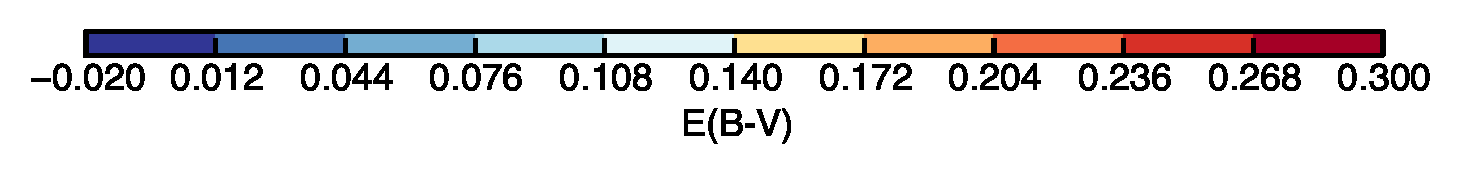
\includegraphics[width=.95\textwidth]{../images/BH/ebv_colorbar}
		\end{column}
	\end{columns}
\end{frame}

\begin{frame}
	\setbeamercovered{transparent}
	\begin{columns}
		\begin{column}{.35\textwidth}
			\begin{block}{Intrinsic color dependent SEDs}
			\begin{itemize}
				\item<1> Bluer quasars have more hot dust and a BBB that peaks at shorter wavelengths
				\item<1> These are both consistent with a hotter accretion disk
				\item<2> The blue quasars have {\em harder} EUV SEDs, contrary to what the spectra indicated
			\end{itemize}
			\end{block}
		\end{column}
		\begin{column}{.75\textwidth}
			\begin{tikzpicture}
				\node[anchor=south west,inner sep=0] (image) at (0,0) {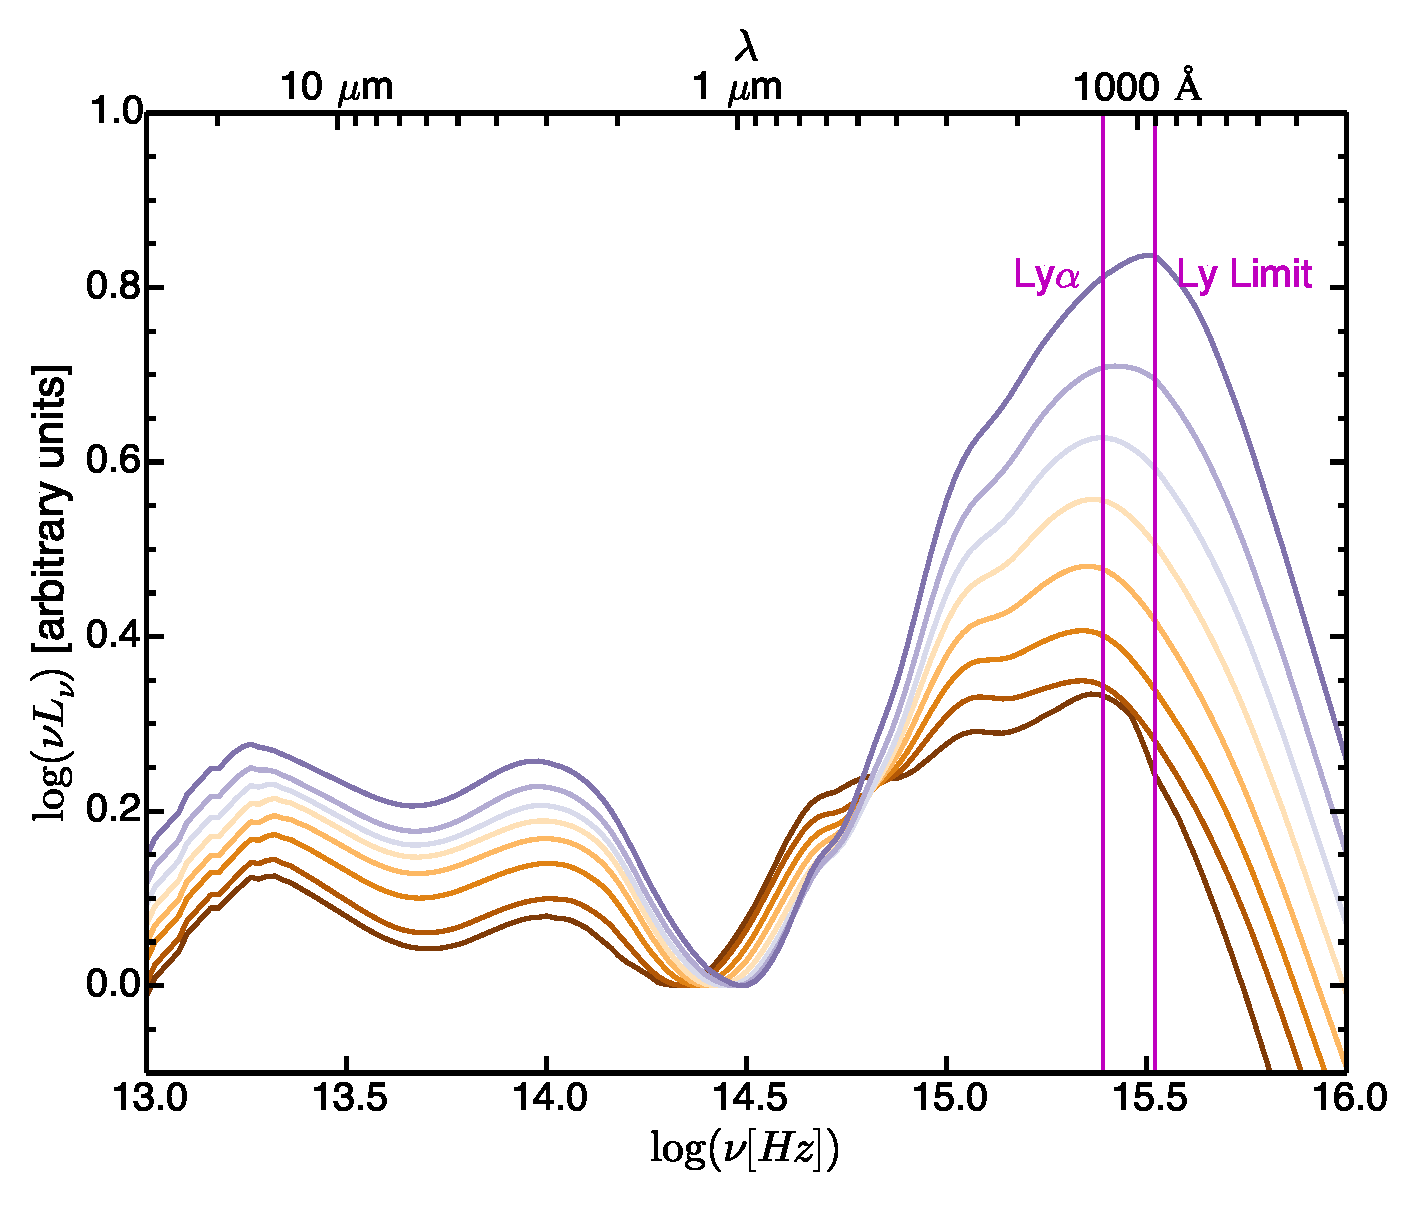
\includegraphics[width=\textwidth]{../images/BH/f4b}};
				\begin{scope}[x={(image.south east)},y={(image.north west)}]
					%\draw<1->[help lines,xstep=.1,ystep=.1] (0,0) grid (1,1);
					\draw<1>[red,ultra thick,->] (.4,.7) -- (.4,.4);
					\draw<1>[red,ultra thick,->] (.5,.8) -- (.75,.8);
					\draw<2>[red,ultra thick] (.9,.5) ellipse (.08 and .45);
				\end{scope}
			\end{tikzpicture}\\
			\hspace{3mm}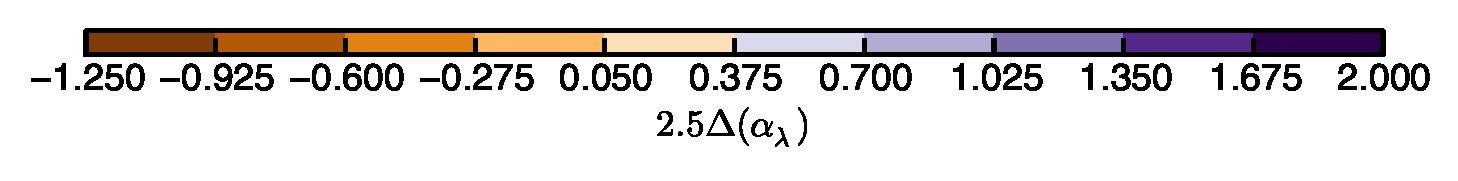
\includegraphics[width=.95\textwidth]{../images/BH/alpha_colorbar}
		\end{column}
	\end{columns}
\end{frame}

\section{Black Hole Properties}
\subsection{Accretion Disks}
\begin{frame}
	\makebox[\textwidth][c]{
	\begin{tikzpicture}
		\node[anchor=south west,inner sep=0] (image) at (0,0) {
			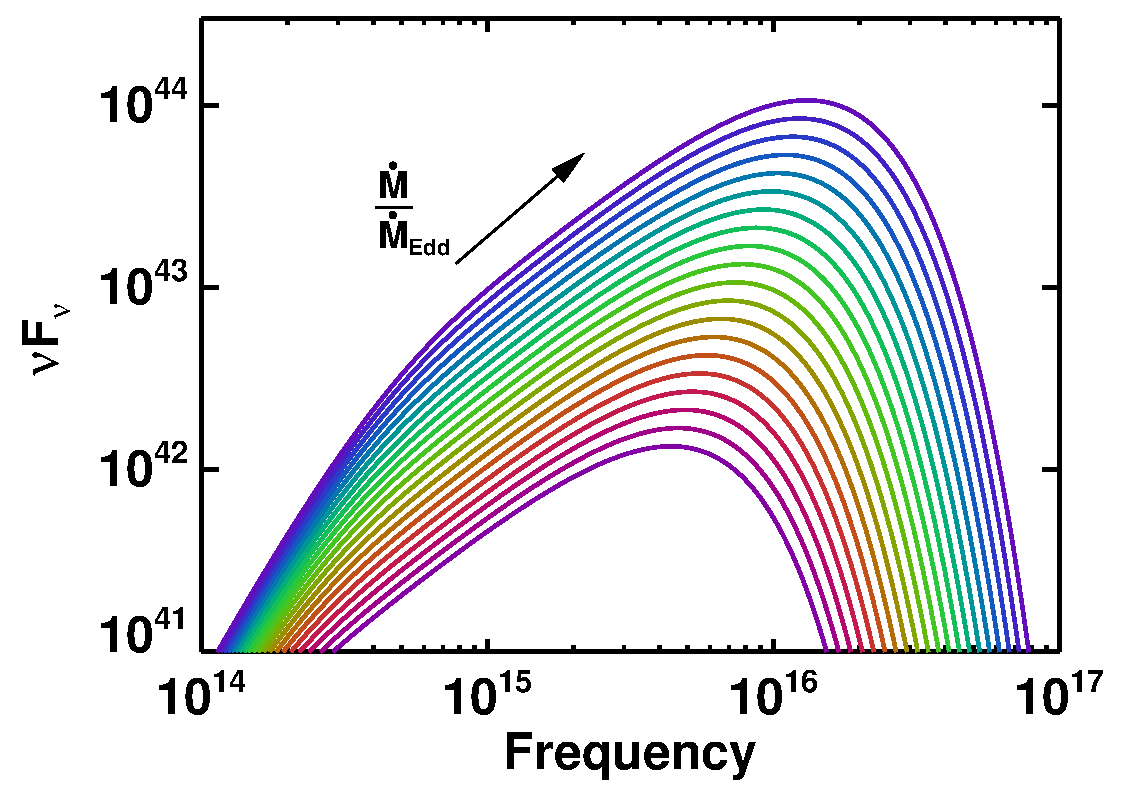
\includegraphics[width=.6\textwidth]{../images/Talk/mdot_out}
			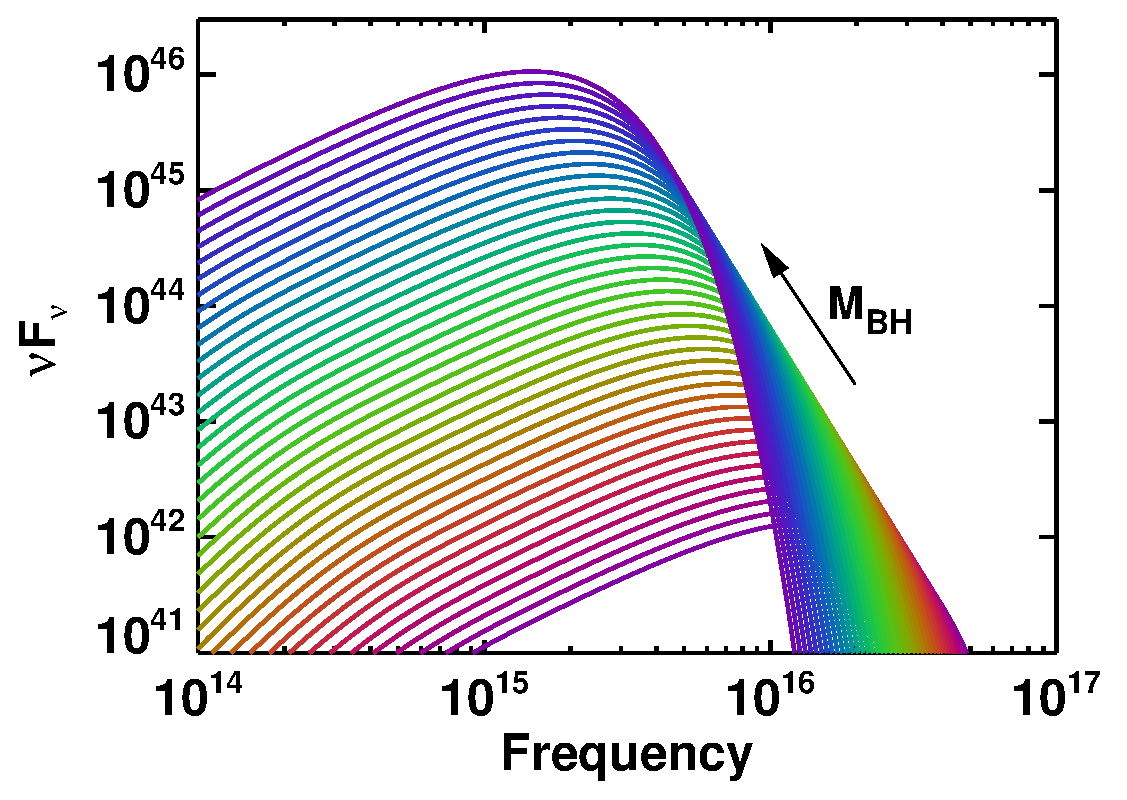
\includegraphics[width=.6\textwidth]{../images/Talk/mbh_out}};
		\begin{scope}[x={(image.south east)},y={(image.north west)}]
			\node at (.85,-.03) {\tiny Plots courtesy of Karen Leighly};
		\end{scope}
	\end{tikzpicture}
	}
	%\vspace{-8mm}
	\begin{block}{$\alpha$-disk \citep{Shakura:1973}}
	\begin{itemize}
		%\item Geometrically thin optically thick accretion disk
		\item Observed SED only dependent on efficiency ($\eta$), BH mass ($M_{BH}$), BH accretion rate ($\dot{M}_{BH}$) 
		%\item $\frac{\dot{M}_{\rm BH}}{\dot{M}_{\rm Edd}} = \frac{L_{\rm Bol}}{L_{\rm Edd}}$
		\item $kT_{eff} \propto \eta^{-1/4} \left( \frac{M_{\rm bh}}{M_\odot} \right)^{-1/4} \left( \frac{\dot{M}}{\dot{M}_{\rm Edd}} \right)^{1/4}$
		% \eta^{-1/4} \left( \frac{M_{\rm bh}}{M_\odot} \right)^{-1/4} \left( \frac{L_{\rm Bol}}{L_{\rm Edd}} \right)^{1/4}$
		%\item Quasars with higher $\frac{L_{bol}}{L_{Edd}}$ or lower $M_{bh}$ will have their SEDs peak further into the UV
	\end{itemize}
	\end{block}
\end{frame}

%\subsection{Black Hole Masses}

\subsection{Mean SEDs}
\begin{frame}
	\begin{columns}
	\begin{column}{.35\textwidth}
		\begin{block}{SEDs grouped by $M_{\rm BH}$}
		\begin{itemize}
			\item The SEDs become bluer as $L/L_{\rm Edd}$ increases
			\item The BBB peaks at shorter wavelengths as $L/L_{\rm Edd}$ increases
			\item Larger $L/L_{\rm Edd}$ is consistent with a hotter accretion disk
			\item This is the same trend predicted by the $\alpha$-disk model
		\end{itemize}
		\end{block}
	\end{column}
	\begin{column}{.75\textwidth}
		\begin{tikzpicture}
			\node[anchor=south west,inner sep=0] (image) at (0,0) {\includegraphics<1->[width=\textwidth]{../images/Talk/f7a}};
			\begin{scope}[x={(image.south east)},y={(image.north west)}]
				\draw[thick,->]  (1,.1) -- (1,.9);
				\node at (1,.95) {$M_{\rm BH}$};
			\end{scope}
		\end{tikzpicture}\\
		\hspace{3mm}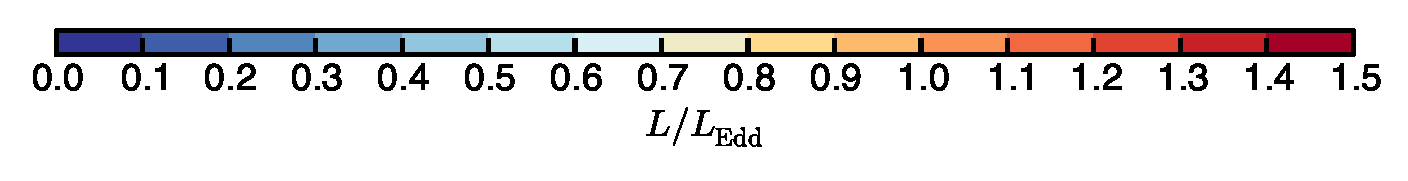
\includegraphics[width=.95\textwidth]{../images/BH/Lf_colorbar}
	\end{column}
	\end{columns}
\end{frame}

\begin{frame}
	\begin{columns}
	\begin{column}{.35\textwidth}
		\begin{block}{SEDs grouped by $L/L_{\rm Edd}$}
		\begin{itemize}
			\item The SEDs become bluer as $M_{\rm BH}$ increases
			\item The BBB peaks at shorter wavelengths as $M_{\rm BH}$ increases
			\item Larger $M_{\rm BH}$ is also consistent with a hotter accretion disk
			\item This is the opposite trend predicted by the $\alpha$-disk model
		\end{itemize}
		\end{block}
	\end{column}
	\begin{column}{.75\textwidth}
		\begin{tikzpicture}
			\node[anchor=south west,inner sep=0] (image) at (0,0) {\includegraphics<1->[width=\textwidth]{../images/Talk/f7b}};
			\begin{scope}[x={(image.south east)},y={(image.north west)}]
				\draw[thick,->] (1,.1) -- (1,.9);
				\node at (1,.98) {$\frac{L}{L_{\rm Edd}}$};
			\end{scope}
		\end{tikzpicture}\\
		\hspace{3mm}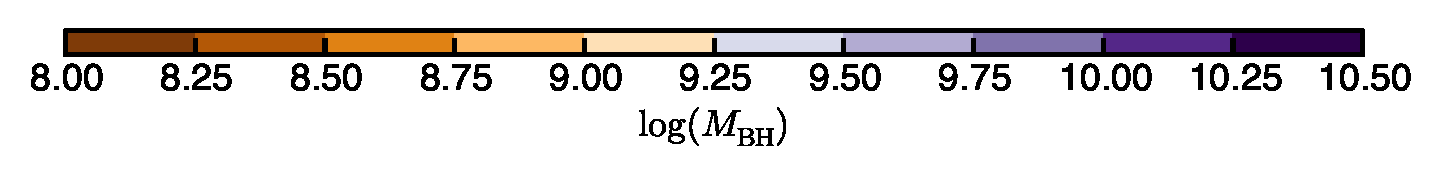
\includegraphics[width=.95\textwidth]{../images/BH/M_colorbar}
	\end{column}
	\end{columns}
\end{frame}

\section{Conclusions}
\subsection{Conclusions 1}
\begin{frame}
	\setbeamercovered{transparent}
	\begin{block}{Mean SEDs}
	\begin{itemize}
		\item<1> We constructed a new mean quasar SED using over 100,000 SDSS selected quasars
		\item<2> We found luminosity trends in the SED shape
		\begin{itemize}
			\item High-luminosity quasars have more hot dust emission
			\item High-luminosity quasars have a softer UV continuum
		\end{itemize}
		\item<3> The range of BCs come from differences in the UV continuum
	\end{itemize}
	\end{block}
	\makebox[\textwidth][c]{
	\includegraphics<1>[width=.5\textwidth]{../images/Talk/f10_crop}
	\includegraphics<2>[width=.5\textwidth]{../images/SEDs/f13a}
	\includegraphics<2>[width=.5\textwidth]{../images/SEDs/f13b}
	\includegraphics<3>[width=.5\textwidth]{../images/SEDs/f13d}
	}
\end{frame}	

\subsection{Conclusions 2}
\begin{frame}
	\setbeamercovered{transparent}
	\begin{block}{Dusty Quasars}
	\begin{itemize}
		\item<1> Using a hierarchical Bayesian model we fit SMC reddening laws to a subset of our data
		\item<1> BAL quasars showed stronger dust extinction than non-BAL quasars
		\item<1> The heavily reddened BAL quasars are bluer than heavily reddened non-BAL quasars
		\item<2> The spectra for the intrinsically blue quasars imply they have a softer EUV continuum than the mean SEDs suggest
		\begin{itemize}
			\item This could happen if the broad line region sees a very different SED than we do
		\end{itemize}
		%\item The size and strength of the absorption troughs in the BAL quasars change in response to the SEDs shape
	\end{itemize}
	\end{block}
	\makebox[\textwidth][c]{
	\includegraphics<1>[width=.3\textwidth]{../images/Talk/f10a}
	\includegraphics<1>[width=.3\textwidth]{../images/Talk/f10B}
	\includegraphics<2>[trim={20.3cm 4cm 0 17.1cm},clip,width=.25\textwidth]{../images/Talk/f12}
	\includegraphics<2>[trim={10cm 22cm 9.25cm 0},clip,width=.5\textwidth]{../images/Dust/f14}
	\includegraphics<2>[width=.3\textwidth]{../images/BH/f4b}
	}
\end{frame}

\subsection{Conclusions 3}
\begin{frame}
	\setbeamercovered{transparent}
	\begin{block}{Black Hole Properties}
	\begin{itemize}
		\item<1> Larger accretion rates lead to hotter accretion disks
		\begin{itemize}
			\item This is consistent with the \citet{Shakura:1973} accretion disk model
		\end{itemize}
		\item<2> Larger black hole masses also lead to hotter accretion disks
		\begin{itemize}
			\item This is {\em not} consistent with the \citet{Shakura:1973} accretion disk model
			\item Deviations from this model could be caused by various effects such as accretion disk winds
		\end{itemize}
	\end{itemize}
	\end{block}
	\makebox[\textwidth][c]{
	\includegraphics<1>[width=.45\textwidth]{../images/Talk/mdot_out}
	\includegraphics<1>[width=.4\textwidth]{../images/Talk/f7a}
	\includegraphics<2>[width=.45\textwidth]{../images/Talk/mbh_out}
	\includegraphics<2>[width=.4\textwidth]{../images/Talk/f7b}
	}
\end{frame}

%\subsection{Future Work}
%\begin{frame}
%	\begin{block}{Future Work}
%	\begin{itemize}
%		\item
%	\end{itemize}
%	\end{block}
%\end{frame}

%===================================
\appendix
\begin{frame}[allowframebreaks]
	%\begin{block}{References}
		\bibliography{../bib/All_refs}
	%\end{block}
\end{frame}

\section{Corrections}
\begin{frame}
	\begin{block}{SED Corrections}
	\begin{itemize}
		\item Lyman--$\alpha$ forest
		\begin{itemize}
			\item The neutral hydrogen between us and the quasar absorbs wavelengths shorter than 912\AA
			\item We use a model for the distribution of these hydrogen clouds to statistically correct for this effect
		\end{itemize}
		\item Strong emission lines
		\begin{itemize}
			\item Strong emission lines can change the shape of the observed SEDs
			\item We remove the effects of these lines by modeling how the filters change in response to the mean quasars spectrum placed at different redshifts
		\end{itemize}
		\item Host galaxy
		\begin{itemize}
			\item Low luminosity quasars are contaminated by host galaxy light in the mid-IR
			\item Using scaling relations from \citet{Shen:2011} and \citet{Richards:2006} we estimate the host galaxy contribution
		\end{itemize}
		\item Gap filling
		\begin{itemize}
			\item Not every filter has data for every quasar
			\item We estimate ``missing'' data in an iteratively based on the mean SED within subsamples of quasars
		\end{itemize}
	\end{itemize}
	\end{block}
\end{frame}

\section{Dust}
%\subsection{Relative Colors}
\begin{frame}
	\begin{columns}
		\begin{column}{0.5\textwidth}
			\centering
			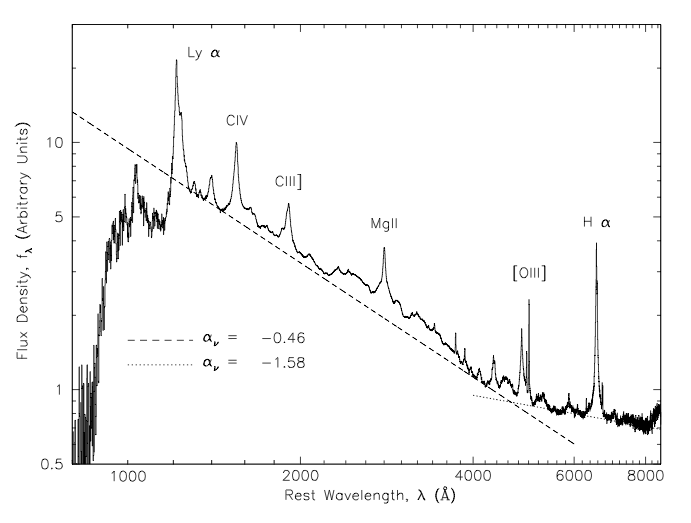
\includegraphics[width=\textwidth]{../images/Talk/vandenberk_01}
			\vspace{-2mm}
			\begin{block}{Modal Colors}
				\begin{itemize}
					\item Strong spectral lines cause trends in the colors of quasars as a function of redshift
					\item Using these trends we can find the ``modal'' quasar color for any given redshift
					%\item{Remove changes in quasar colors that are due to spectral lines shifting through the filters}
					%\item{Slopes in the relative colors indicate quasars that are intrinsically redder/bluer than the mode}
					%\item{Curvature in the relative colors indicate dust reddening}
				\end{itemize}
			\end{block}
		\end{column}
		\begin{column}{0.6\textwidth}
			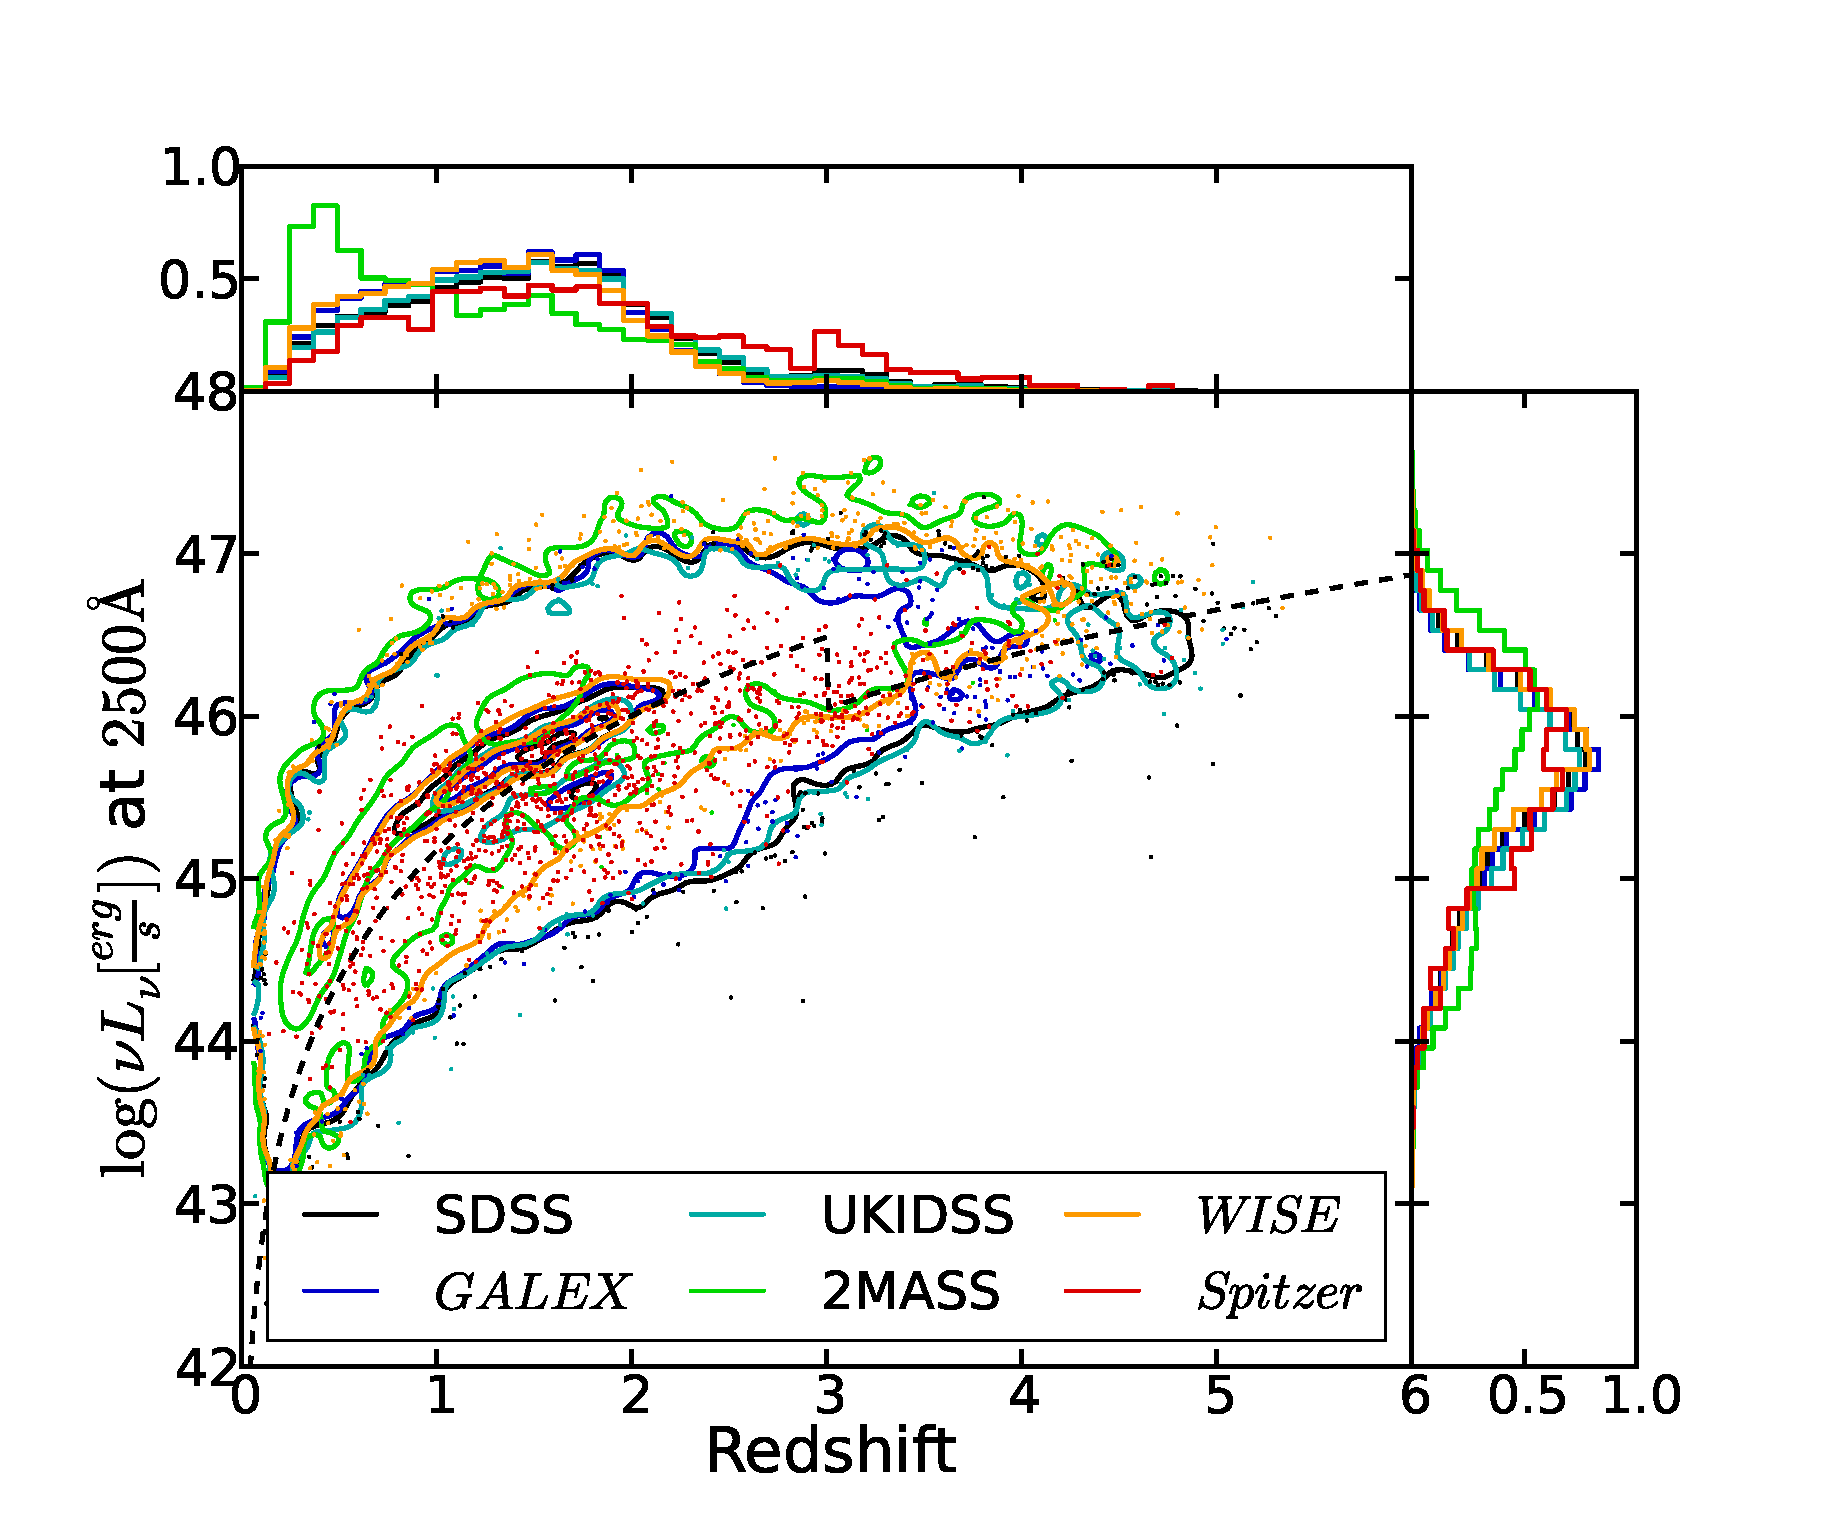
\includegraphics[width=.985\textwidth]{../images/Dust/f2}
		\end{column}
	\end{columns}
\end{frame}

%\subsection{L14 Reddening Law}
\begin{frame}[label=L14_fits]
	\begin{columns}
		\begin{column}{0.45\textwidth}
			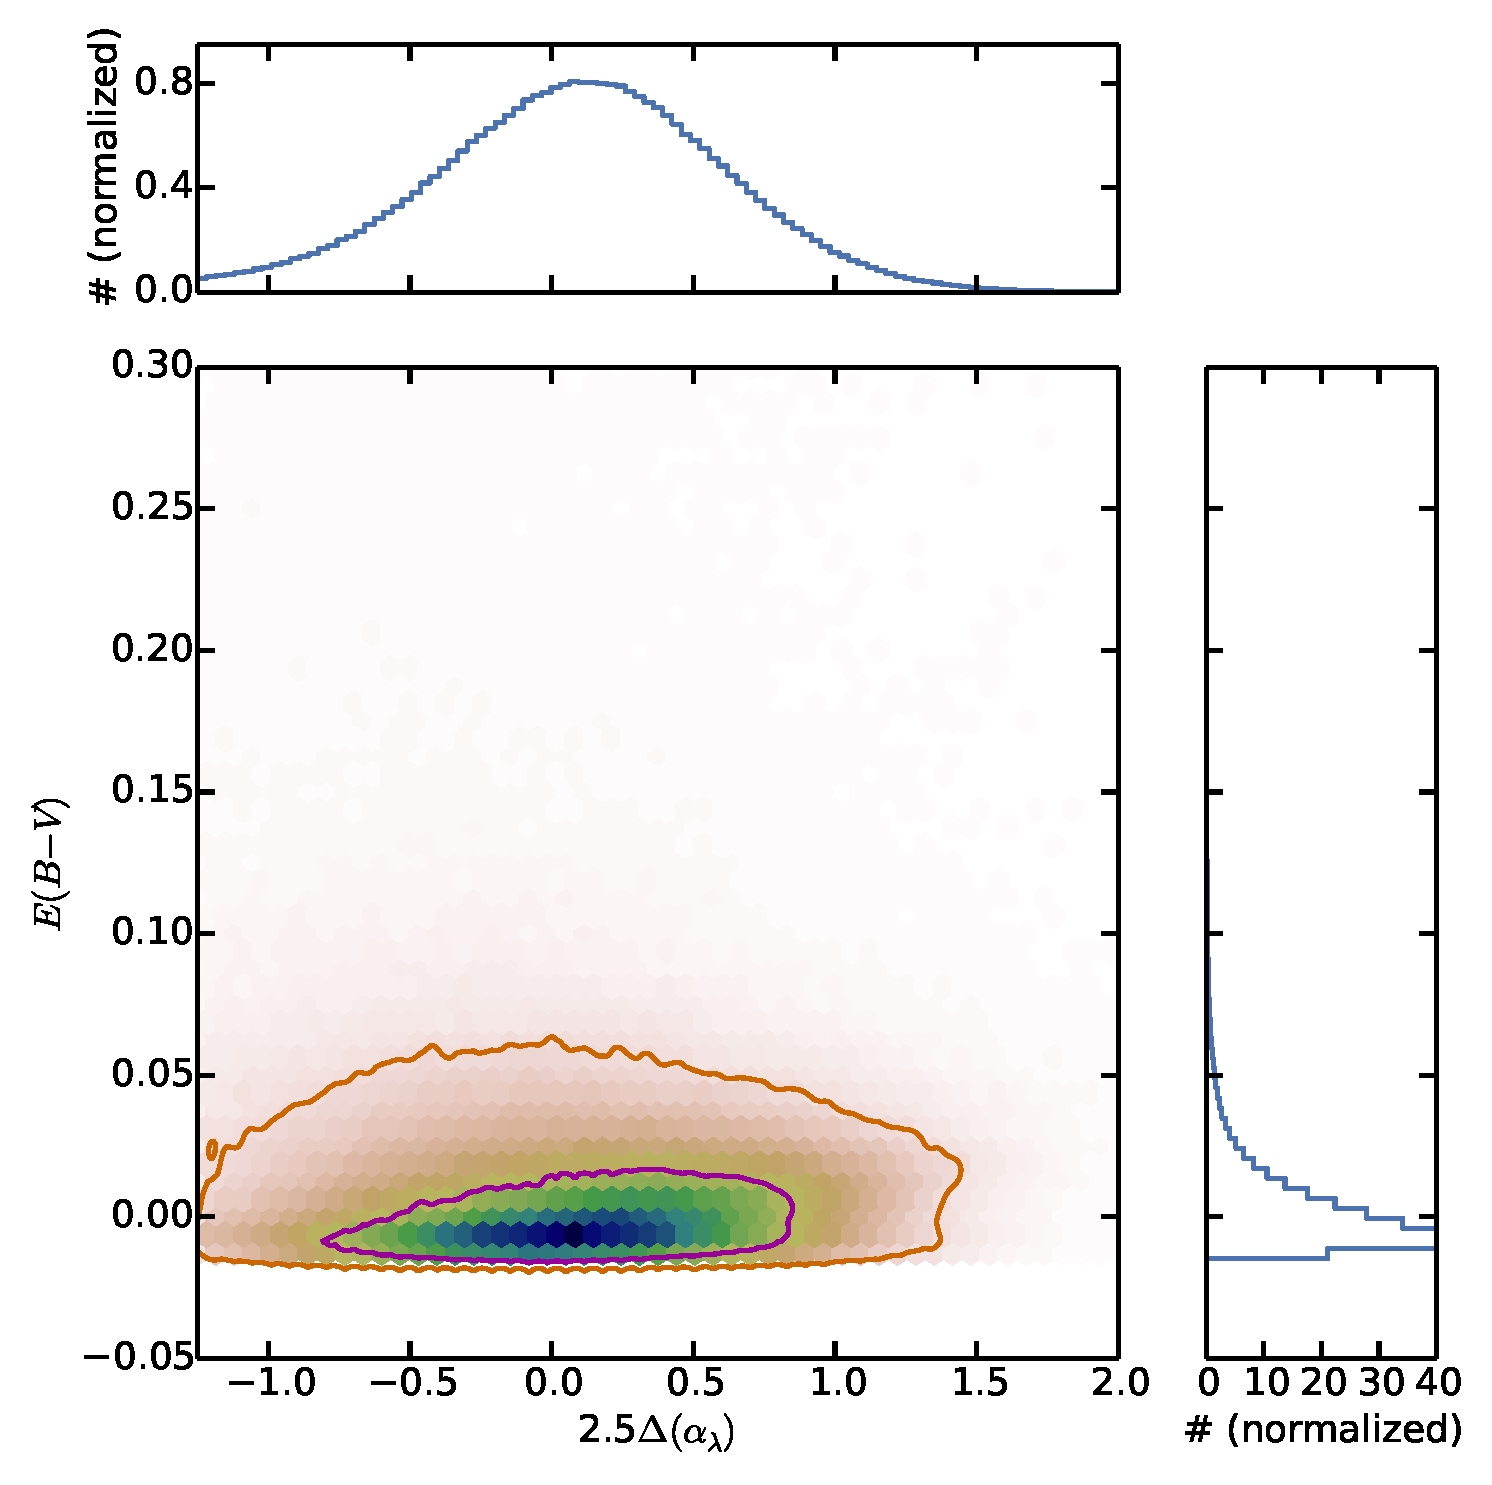
\includegraphics[width=\textwidth]{../images/Dust/f10c}
		\end{column}
		\begin{column}{0.45\textwidth}
			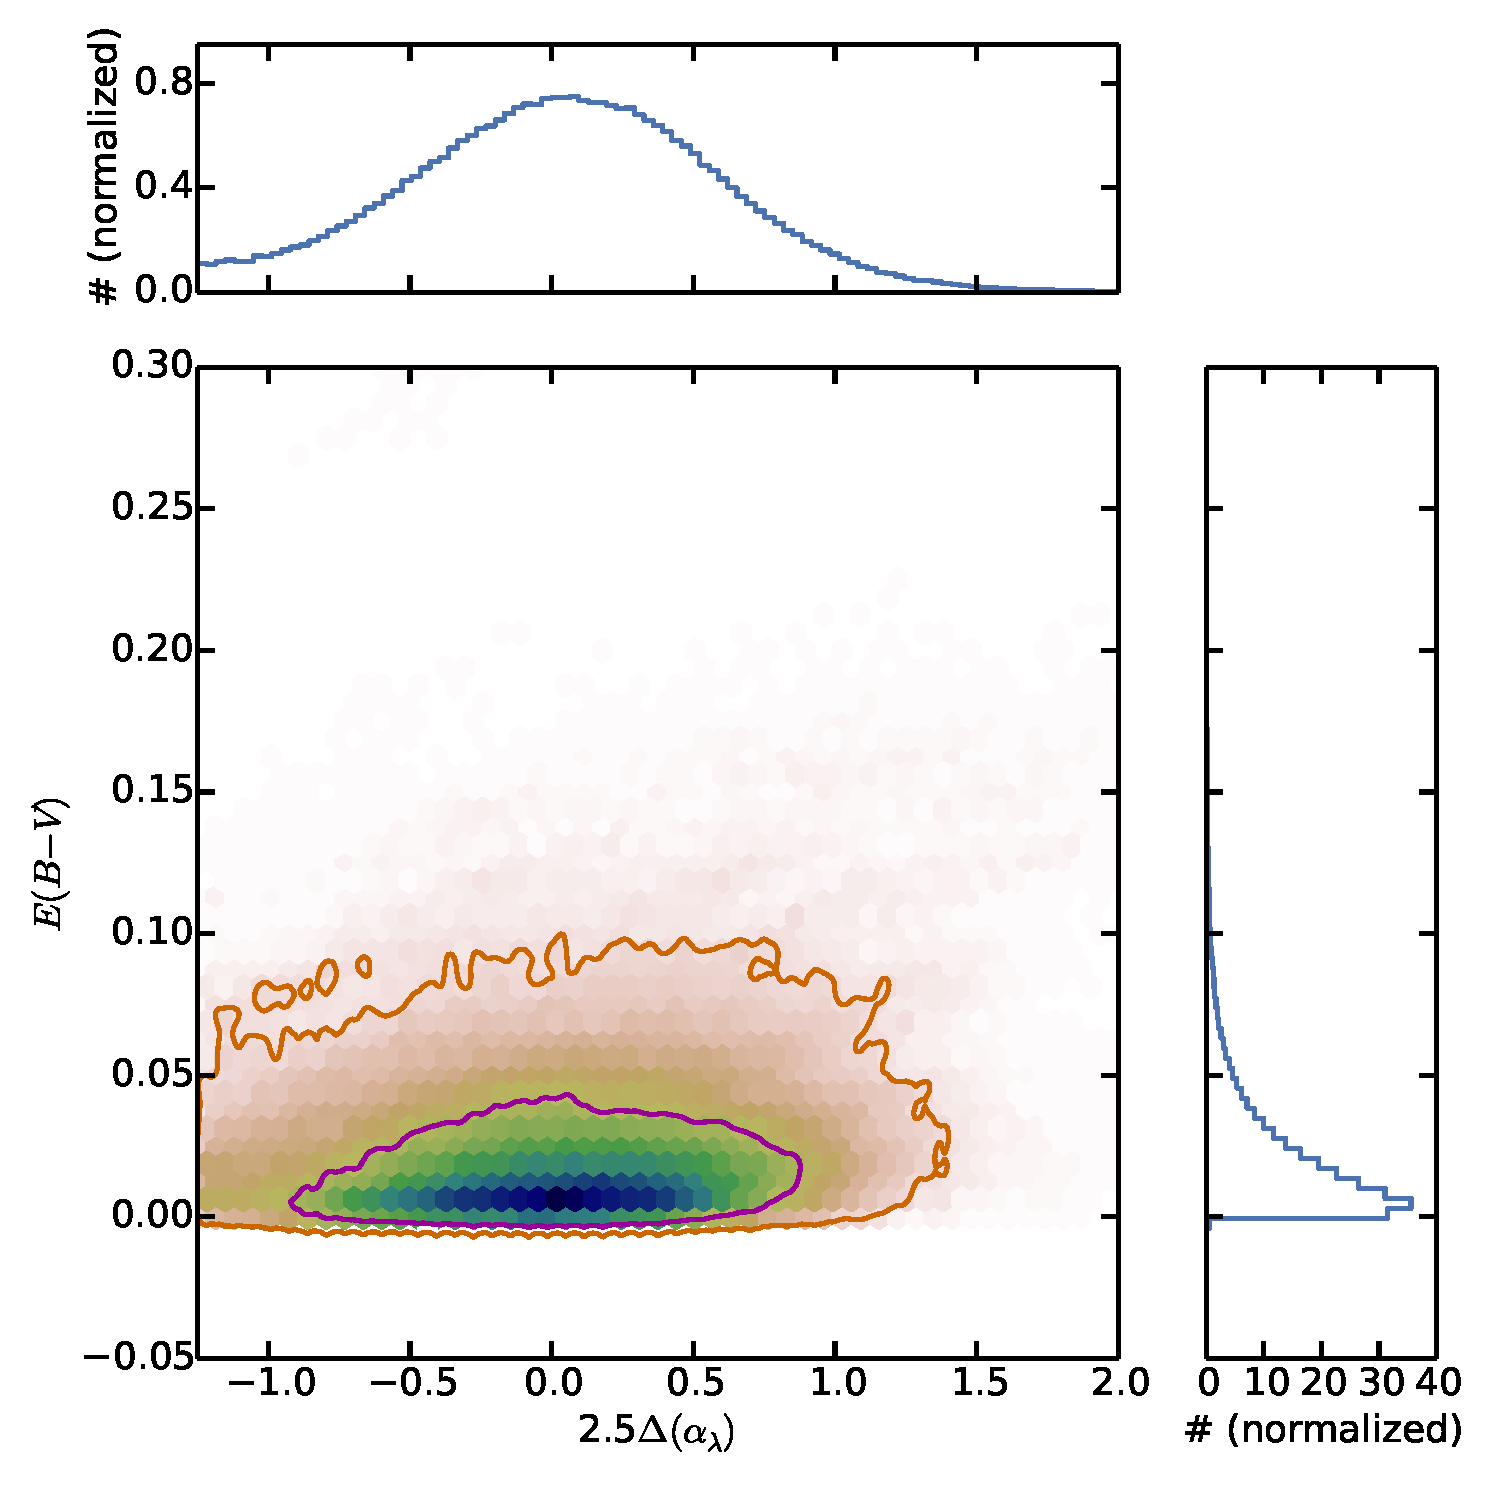
\includegraphics[width=\textwidth]{../images/Dust/f10d}
		\end{column}
	\end{columns}
	\begin{block}{L14-QSO fit}
		\begin{itemize}
			\item{Both samples have lower E(B-V) values than before}
			\item{The BAL sample is slightly redder than the the non-BAL sample}
		\end{itemize}
	\end{block}
	%\hyperlink{SMC_fits}{\beamerbutton{here}}
\end{frame}

%\subsection{BAL Fraction}
\begin{frame}
	\begin{columns}
		\begin{column}{0.4\textwidth}
			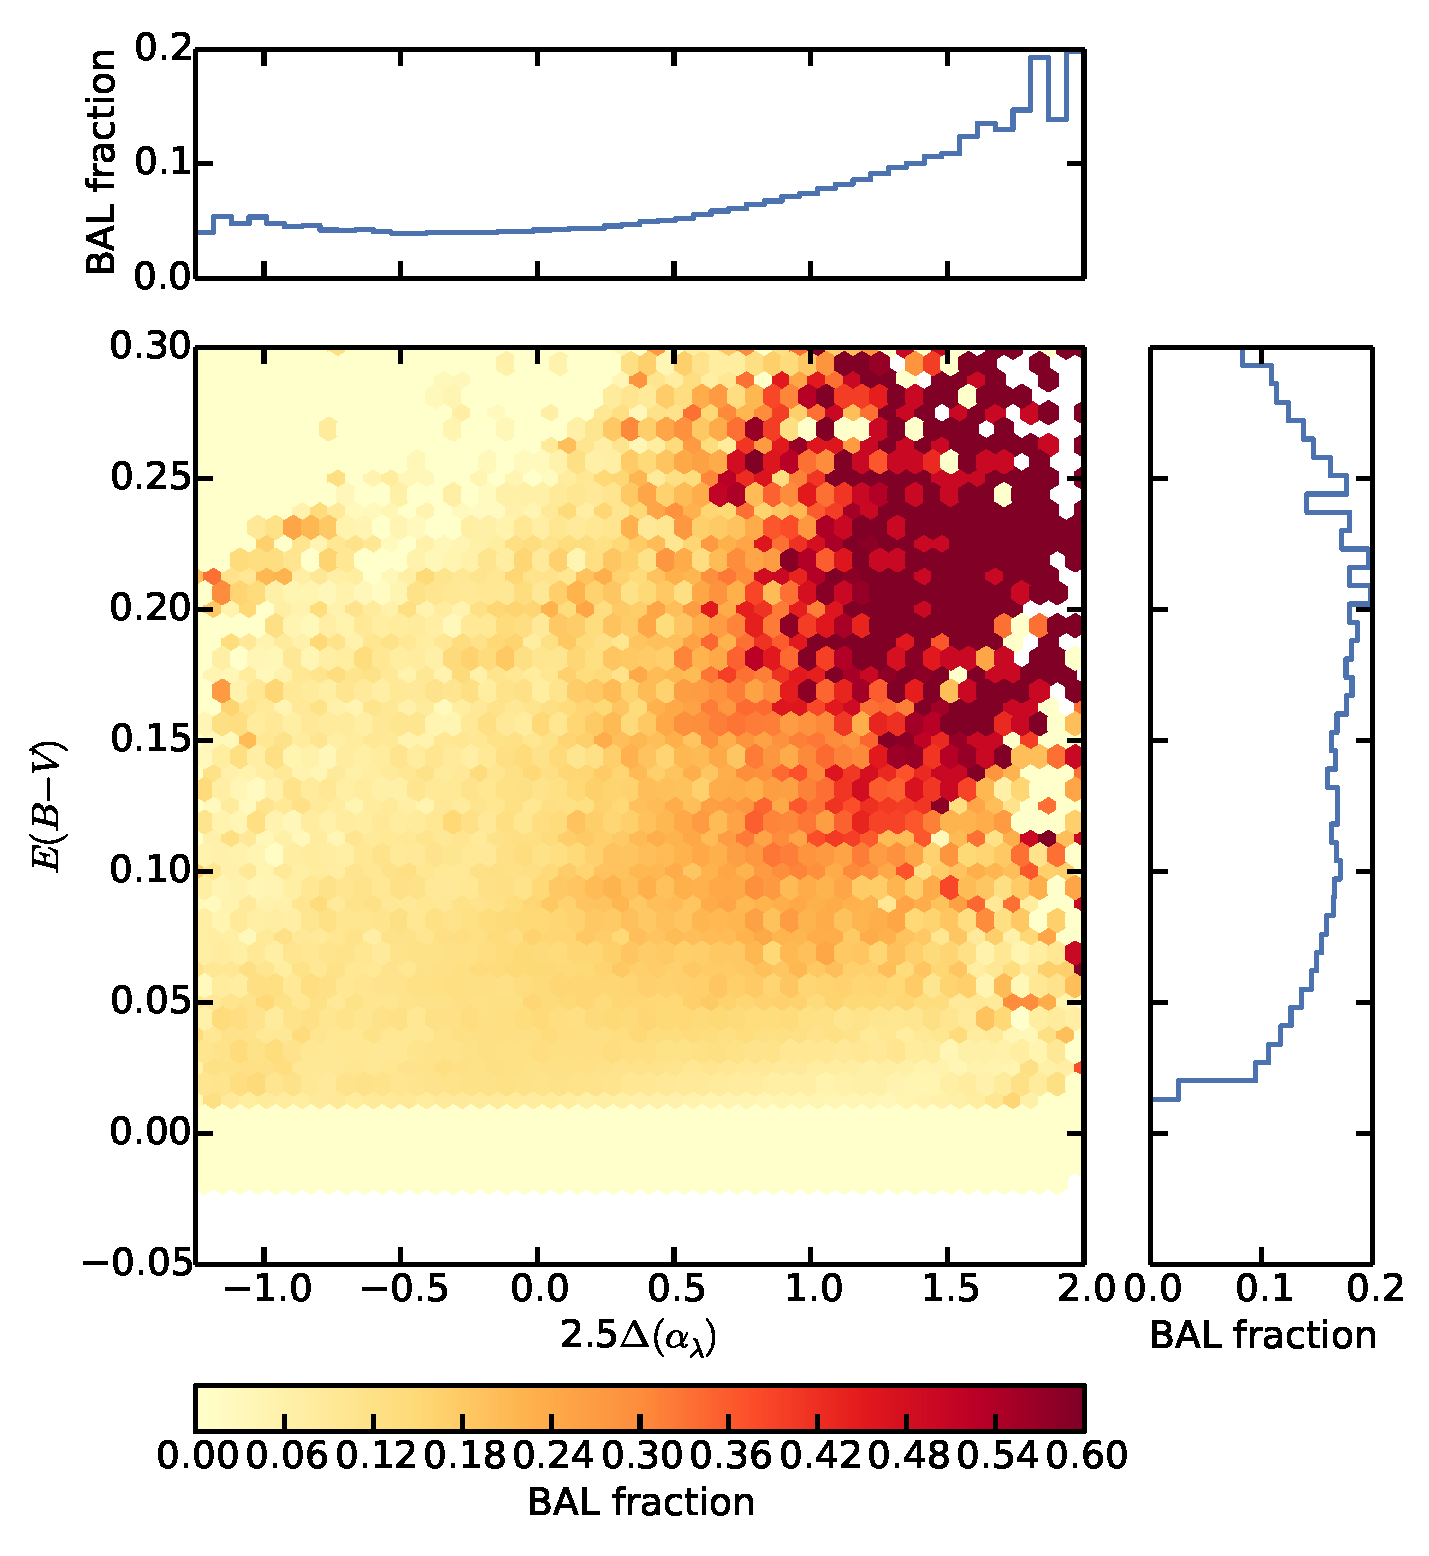
\includegraphics[width=\textwidth]{../images/Dust/f11a}
		\end{column}
		\begin{column}{0.4\textwidth}
			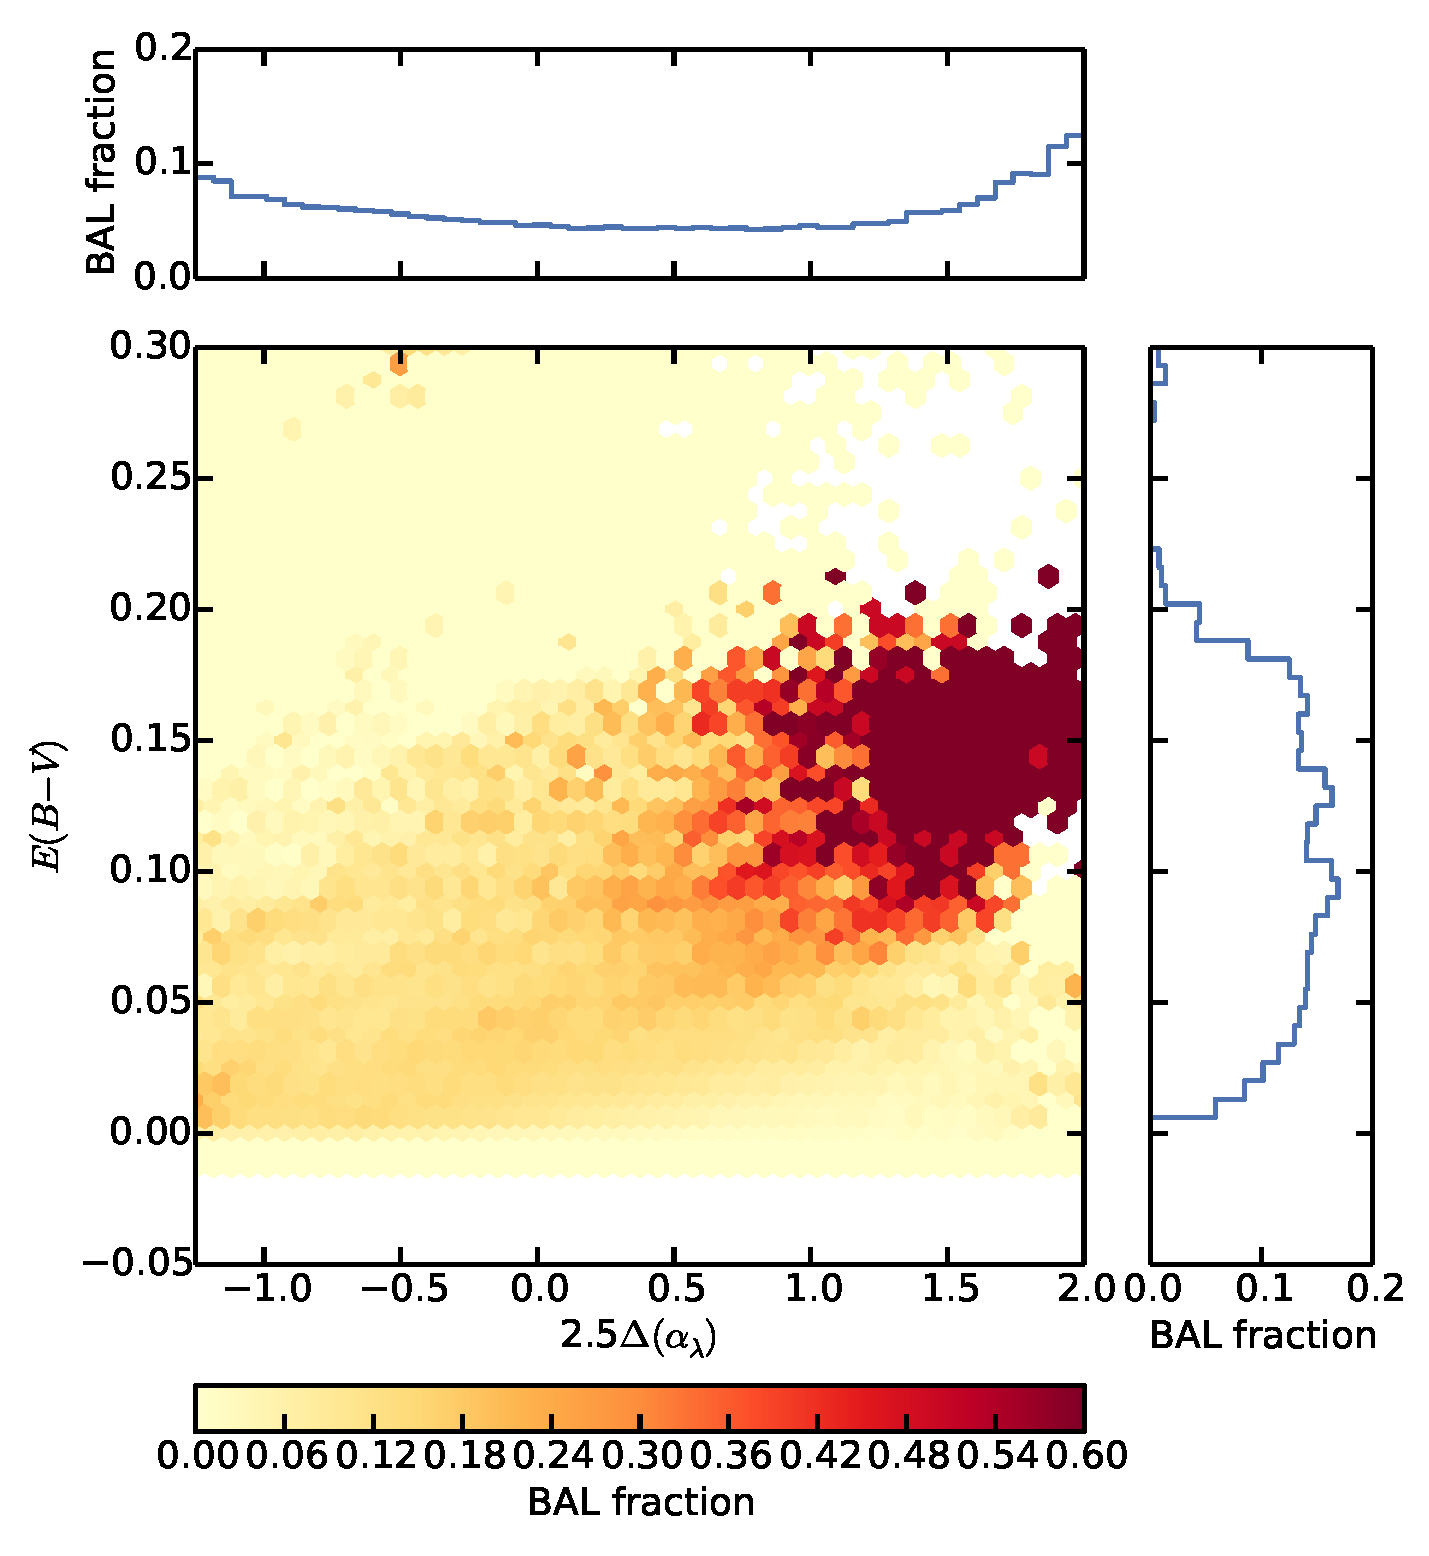
\includegraphics[width=\textwidth]{../images/Dust/f11b}
		\end{column}
	\end{columns}
	\vspace{-2mm}
	\begin{block}{BAL fraction}
		\begin{itemize}
			\item{The BAL fraction ranges from $\sim$0.05--0.2 as the $\Delta(\alpha_\lambda)$ value changes for both dust laws}
			\item{BAL quasars dominate the intrinsically blue and highly reddened part of the parameter space}
		\end{itemize}
	\end{block}
\end{frame}

%\subsection{Choosing a Reddening Law}
\begin{frame}
	\vspace{-2mm}
	\begin{block}{Deviance Information Criterion (DIC)}
		\begin{itemize}
			\item{Bayesian analysis allows for the direct comparison of multiple models}
			\item{Looking at the difference between the DIC values between the two models tells us what one fits better}
		\end{itemize}
	\end{block}
	\begin{block}{What model fits better}
	\begin{itemize}
		\item{non-BAL quasars}
		\begin{itemize}
			\item{SMC: 95.6\%}
			\item{either model: 4.3\%}
			\item{L14-QSO: 0.06\%}
		\end{itemize}
		\item{BAL quasars}
		\begin{itemize}
			\item{SMC: 88.6\%}
			\item{either model: 11\%}
			\item{L14-QSO: 0.4\%}
		\end{itemize}
	\end{itemize}
	\end{block}
\end{frame}

%\subsection{BAL Spectra}
\begin{frame}
	\begin{columns}
		\begin{column}{0.35\textwidth}
			\begin{block}{SMC BAL}
			\begin{itemize}
				\item As before, the fits based on the photometry track the spectra well
				\item The depth of the \ion{C}{4} absorption trough increases with E(B-V)
				\item The width of the \ion{C}{4} absorption trough increases with intrinsic color
			\end{itemize}
			\end{block}
		\end{column}
		\begin{column}{0.7\textwidth}
			\begin{tikzpicture}
				\node[anchor=south west,inner sep=0] (image) at (0,0) {\includegraphics<1->[width=\textwidth]{../images/Talk/f13}};
				\begin{scope}[x={(image.south east)},y={(image.north west)}]
					\draw<2>[red,ultra thick] (.16,.855) ellipse (.03 and .13);
					\draw<2>[red,ultra thick] (.16,.58) ellipse (.03 and .13);
					\draw<2>[red,ultra thick] (.16,.3) ellipse (.03 and .13);
					\draw<2>[red,ultra thick] (.465,.855) ellipse (.03 and .13);
					\draw<2>[red,ultra thick] (.465,.58) ellipse (.03 and .13);
					\draw<2>[red,ultra thick] (.465,.3) ellipse (.03 and .13);
					\draw<2>[red,ultra thick] (.77,.855) ellipse (.03 and .13);
					\draw<2>[red,ultra thick] (.77,.58) ellipse (.03 and .13);
					\draw<2>[red,ultra thick] (.77,.3) ellipse (.03 and .13);
				\end{scope}
			\end{tikzpicture}
		\end{column}
	\end{columns}
\end{frame}

\begin{frame}
	\begin{columns}
	\begin{column}{.35\textwidth}
		\begin{block}{BAL Spectral Lines}
		\begin{itemize}
			\item The shape/size of the absorption troughs is correlated with SED shape
			\item The narrow, low velocity absorption in the redder BALs could be an indication of a weaker wind or a higher RL fraction
			\item \ion{C}{4} and \ion{C}{3}] shows similar emission line trends as the non-BAL spectra
		\end{itemize}
		\end{block}
	\end{column}
	\begin{column}{.75\textwidth}
		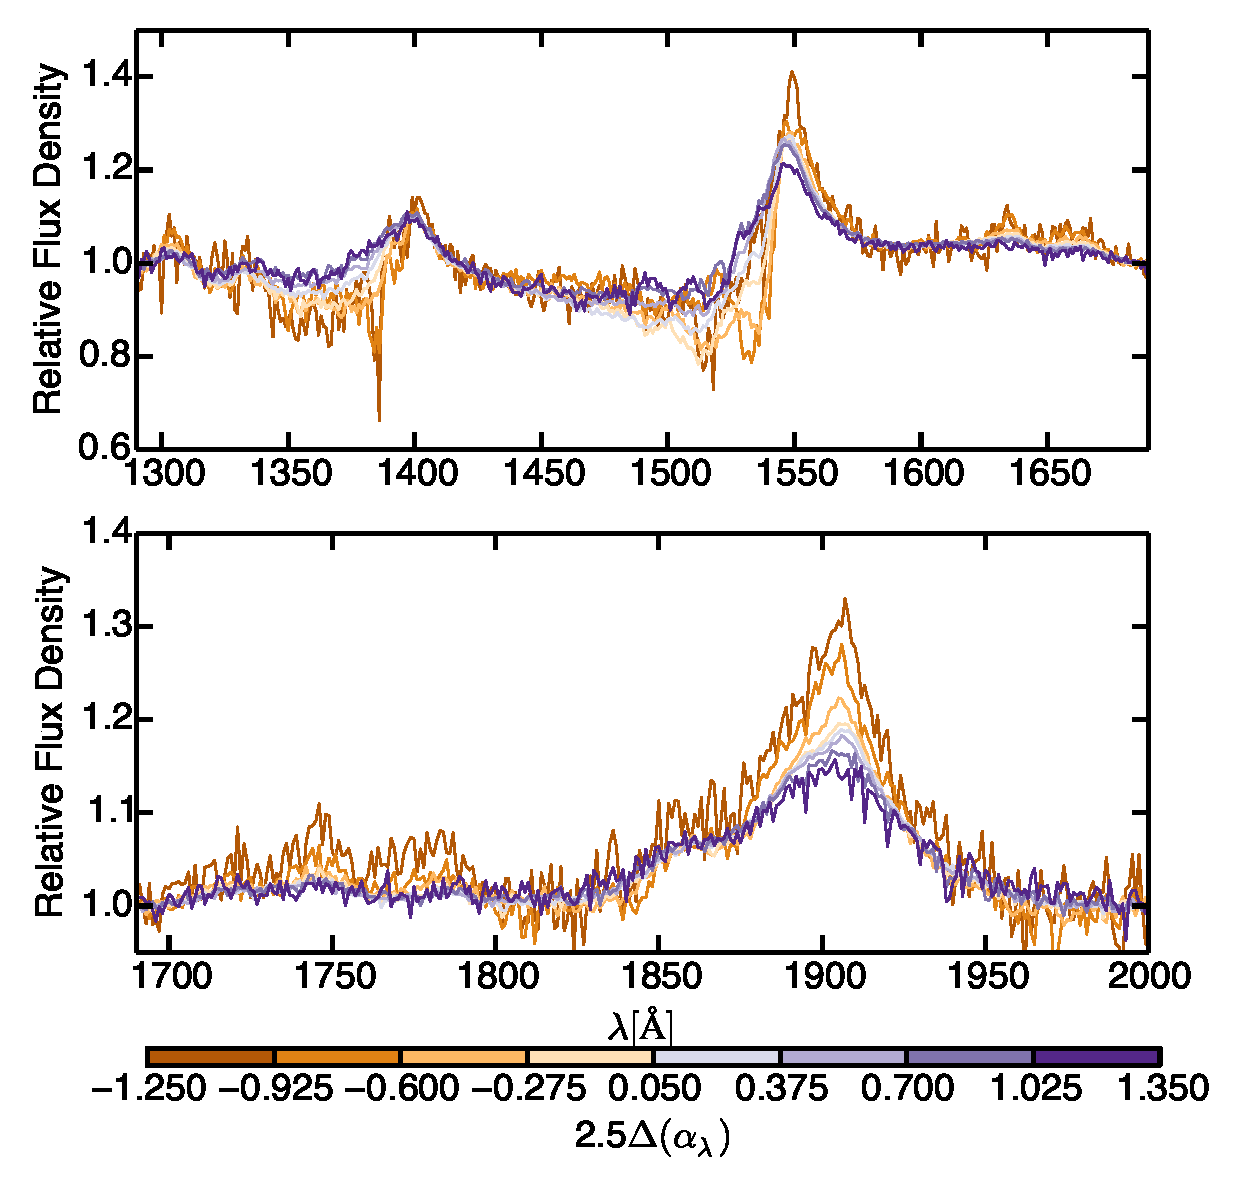
\includegraphics[width=\textwidth]{../images/Dust/f15}
	\end{column}
	\end{columns}
\end{frame}

%\subsection{Extinction Correction}
\begin{frame}
	\begin{columns}
		\begin{column}{.35\textwidth}
			\begin{block}{Dust Correction}
			\begin{itemize}
				\item Dust extinction correction for a quasar with E(B-V)=0.2
				\item Red: Observed SED
				\item Blue: Corrected SED
				\item Less then $0.1\%$ of our sample needs a correction this extreme
			\end{itemize}
			\end{block}
		\end{column}
		\begin{column}{.75\textwidth}
			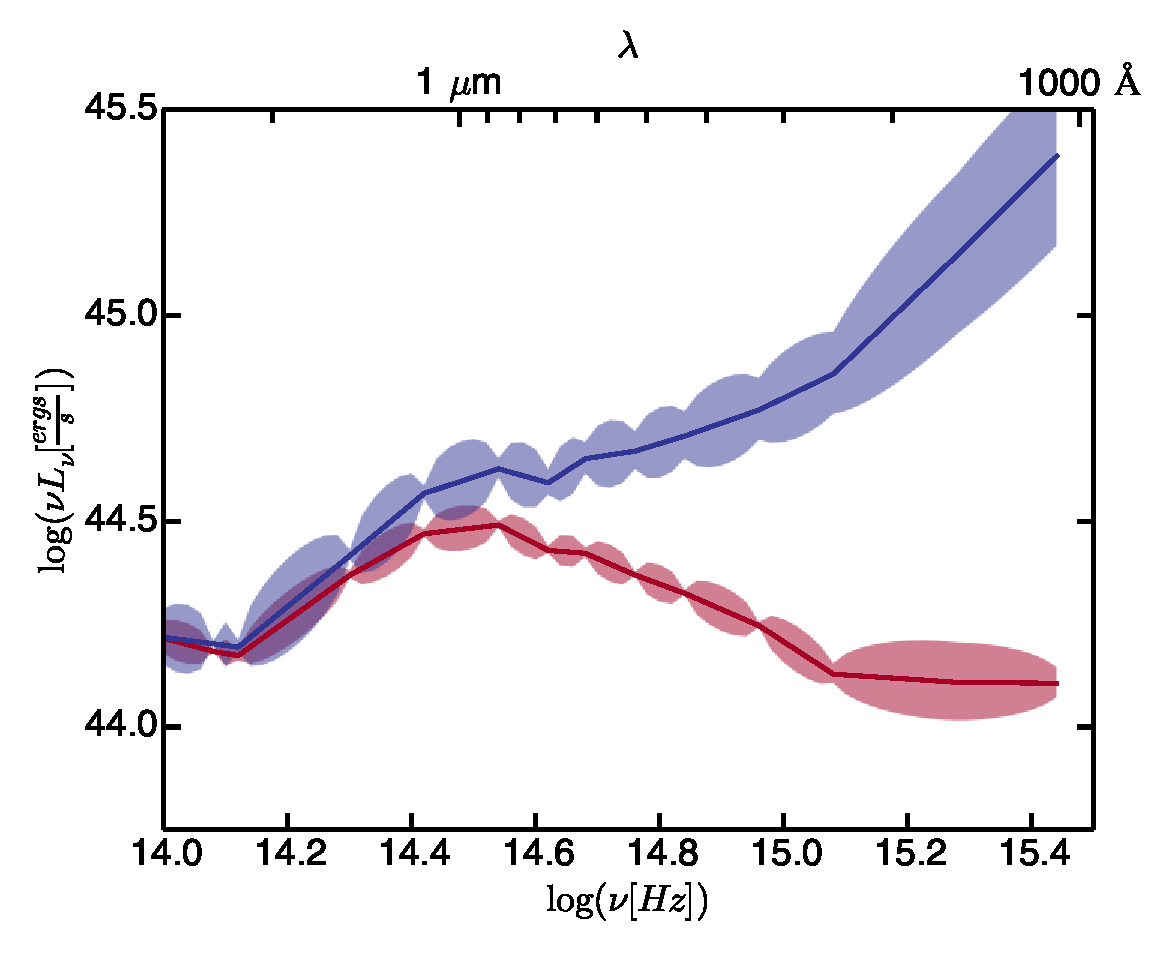
\includegraphics[width=\textwidth]{../images/BH/f2}
		\end{column}
	\end{columns}
\end{frame}

%\subsection{Luminosity and BCs}
\begin{frame}
	\begin{columns}
	\begin{column}{.35\textwidth}
		\begin{block}{Luminosity and \\ BC distributions}
		\begin{itemize}
			\item More reddened quasars have higher luminosities, and as a result, lower BCs
			\item There are no luminosity trends with intrinsic color, but the bluer quasars have larger BCs
		\end{itemize}
		\end{block}
	\end{column}
	\begin{column}{.75\textwidth}
		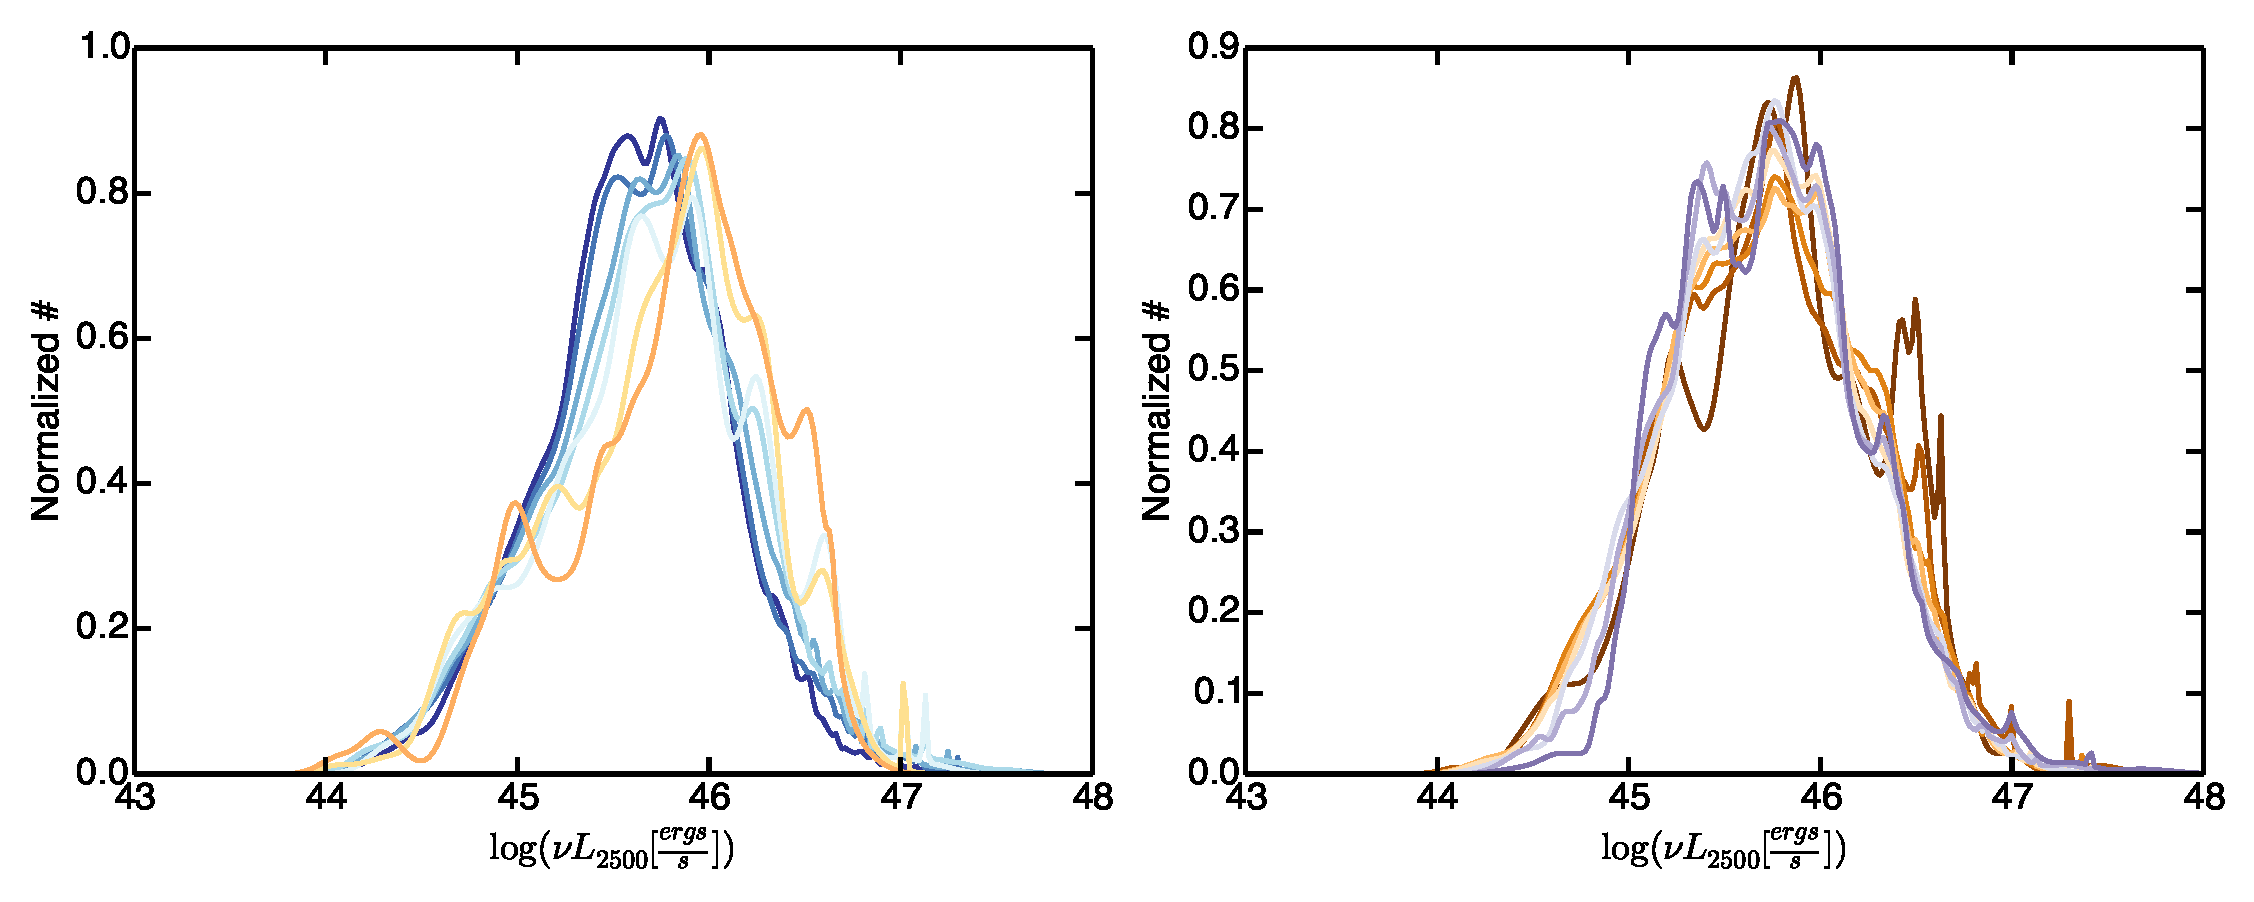
\includegraphics[width=\textwidth]{../images/BH/f6a}\\
		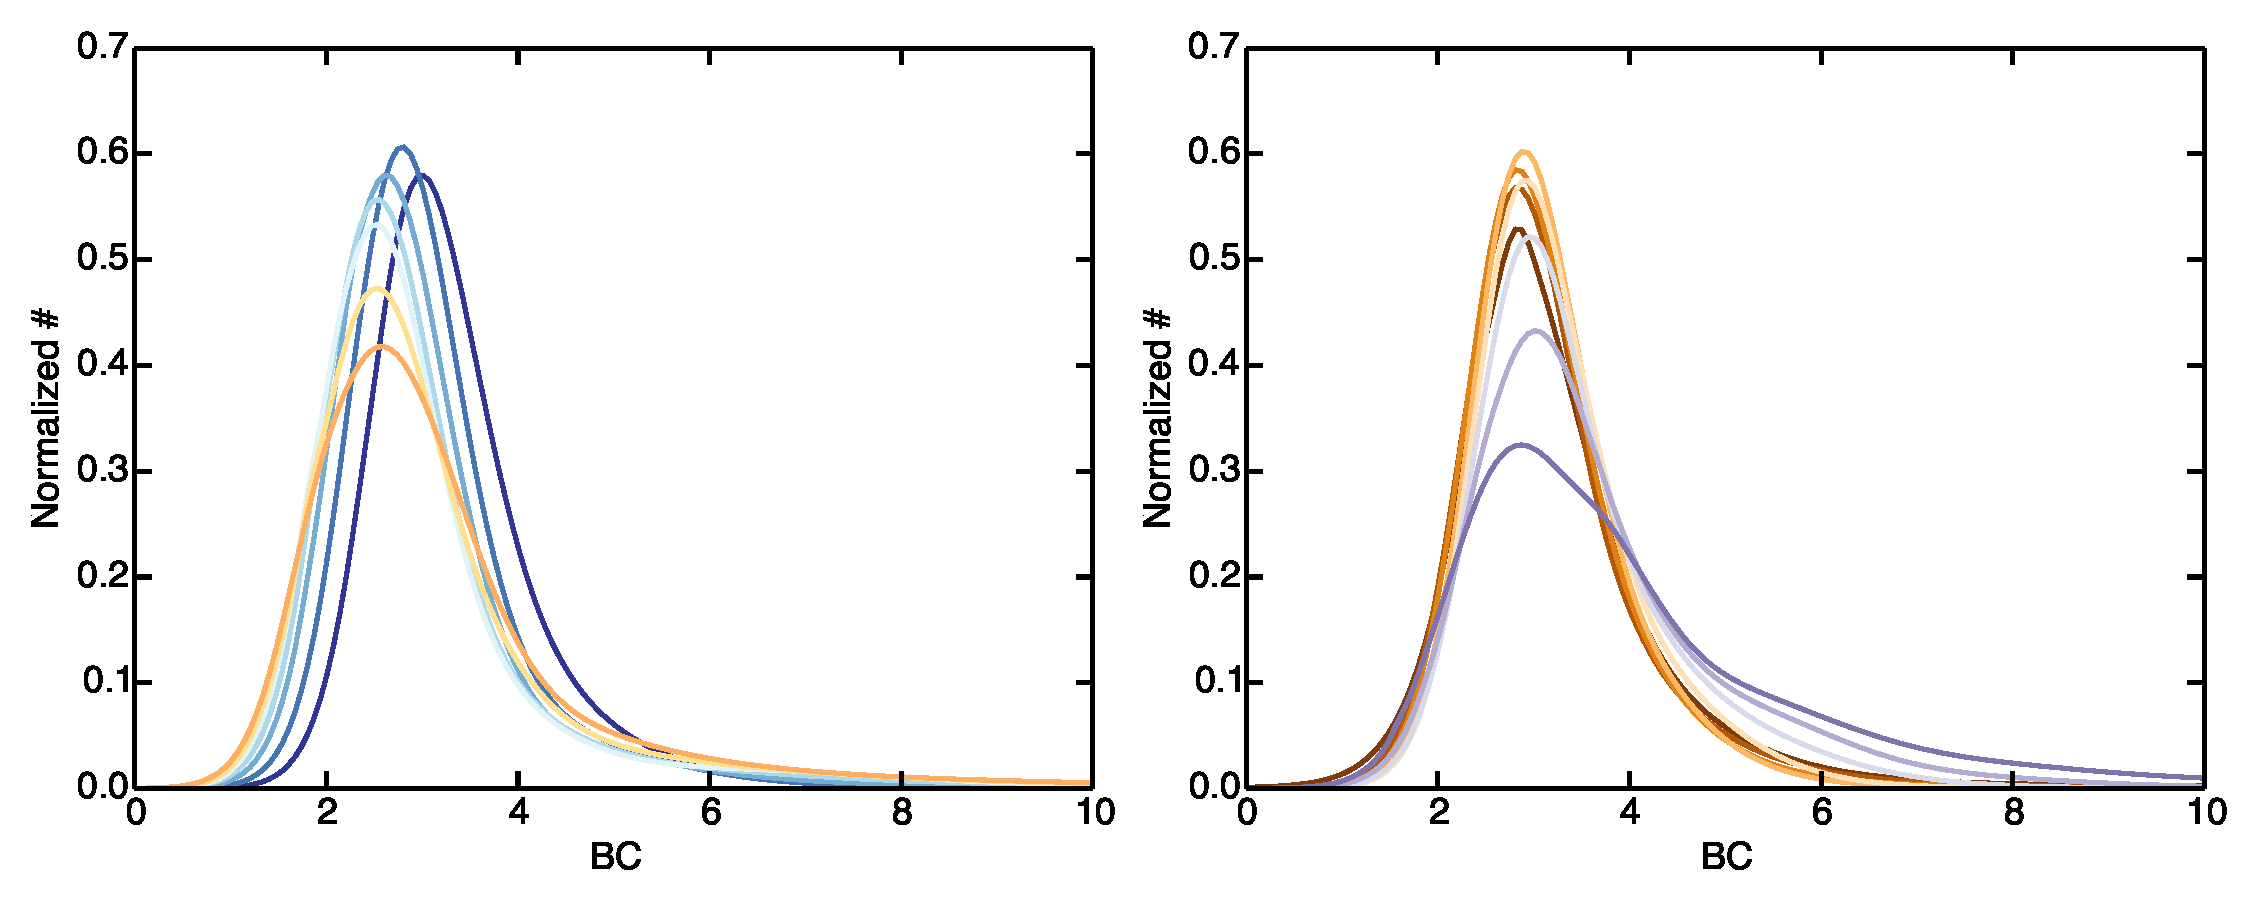
\includegraphics[width=\textwidth]{../images/BH/f6b}\\
		\hspace{2mm}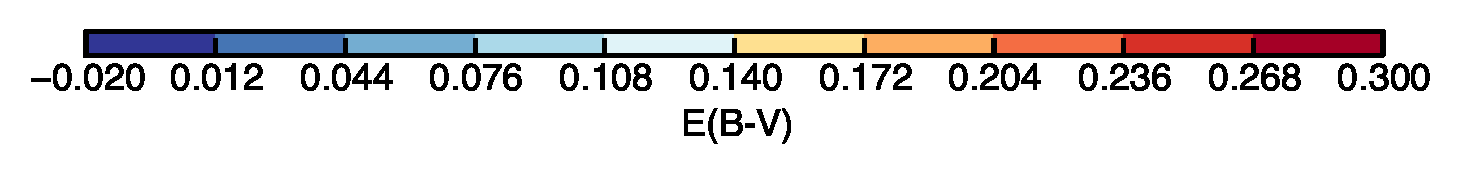
\includegraphics[width=.47\textwidth]{../images/BH/ebv_colorbar} 
		\hspace{2.5mm}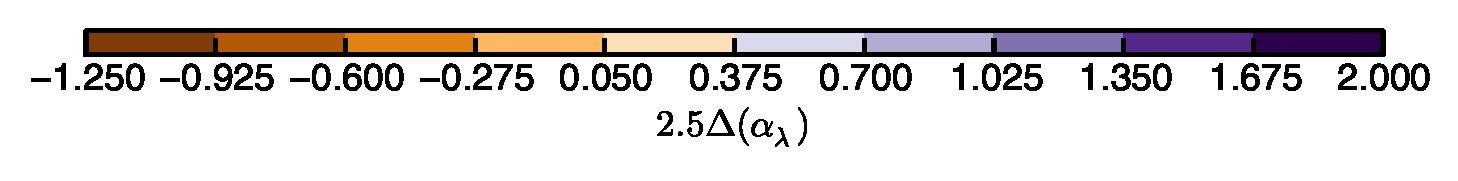
\includegraphics[width=.47\textwidth]{../images/BH/alpha_colorbar}
	\end{column}
	\end{columns}
\end{frame}

\section{Black Hole Properties}
\begin{frame}
	\begin{columns}
	\begin{column}{.35\textwidth}
		\begin{block}{Central black hole masses}
		\begin{itemize}
			\item Estimated from emission line widths %(relations calibrated using reverberation mapping data)
			%\item Started with the mass estimates cataloged in \citet{Shen:2011}
			\item Started with a catalog of masses estimated using the FWHM of various broad lines
			%\item Applied re-calibrations for these masses found by \citet{Rafiee:2011} and \citet{Park:2013}
			\item Applied re-calibrations to account for the FWHM over estimating the masses
		\end{itemize}
		\end{block}
	\end{column}
	\begin{column}{.75\textwidth}
		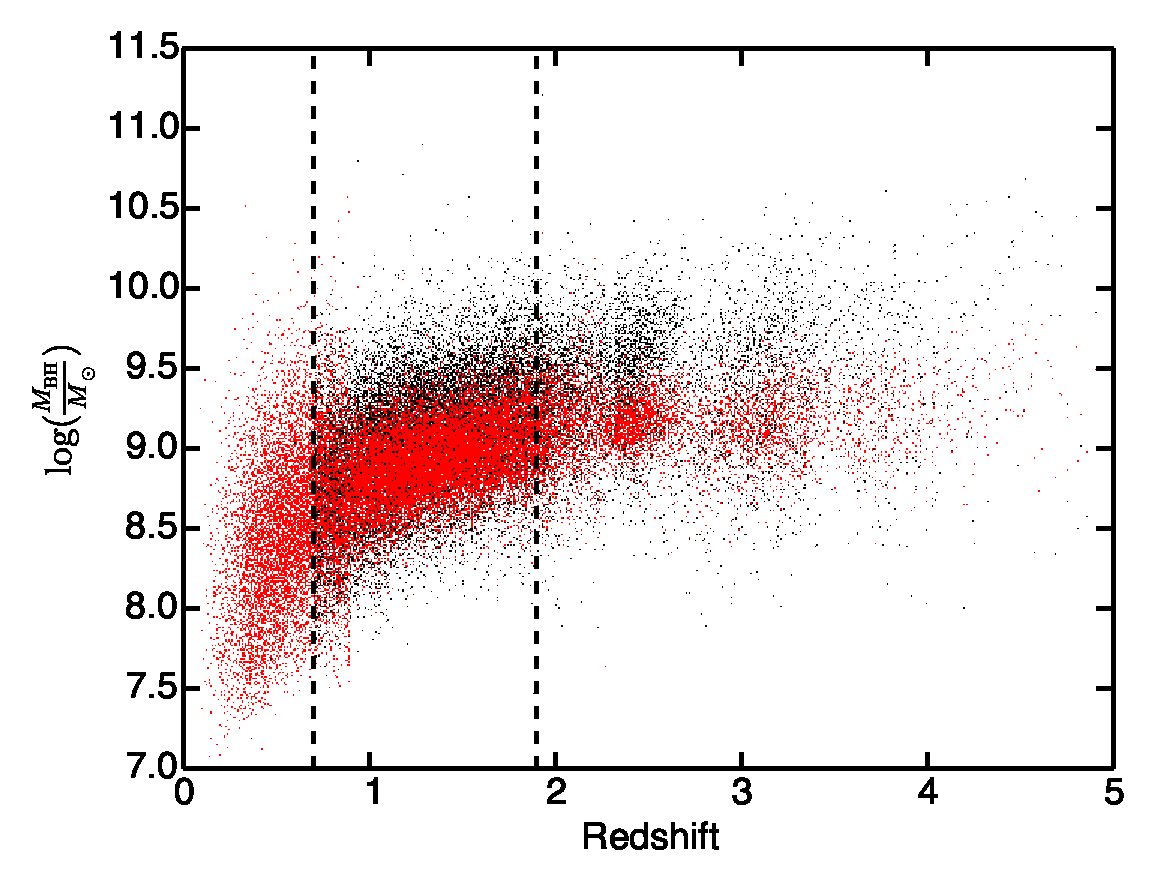
\includegraphics[width=\textwidth]{../images/BH/f1}
	\end{column}
	\end{columns}
\end{frame}

%\subsection{Luminosity and BCs}
\begin{frame}
	\begin{columns}
	\begin{column}{.35\textwidth}
		\begin{block}{Luminosity and \\ BC distributions}
		\begin{itemize}
			\item Quasars with hither accretion rates have higher luminosities and higher BCs
			\item More massive quasars have slightly higher luminosities and no trends with BC
		\end{itemize}
		\end{block}
	\end{column}
	\begin{column}{.75\textwidth}
		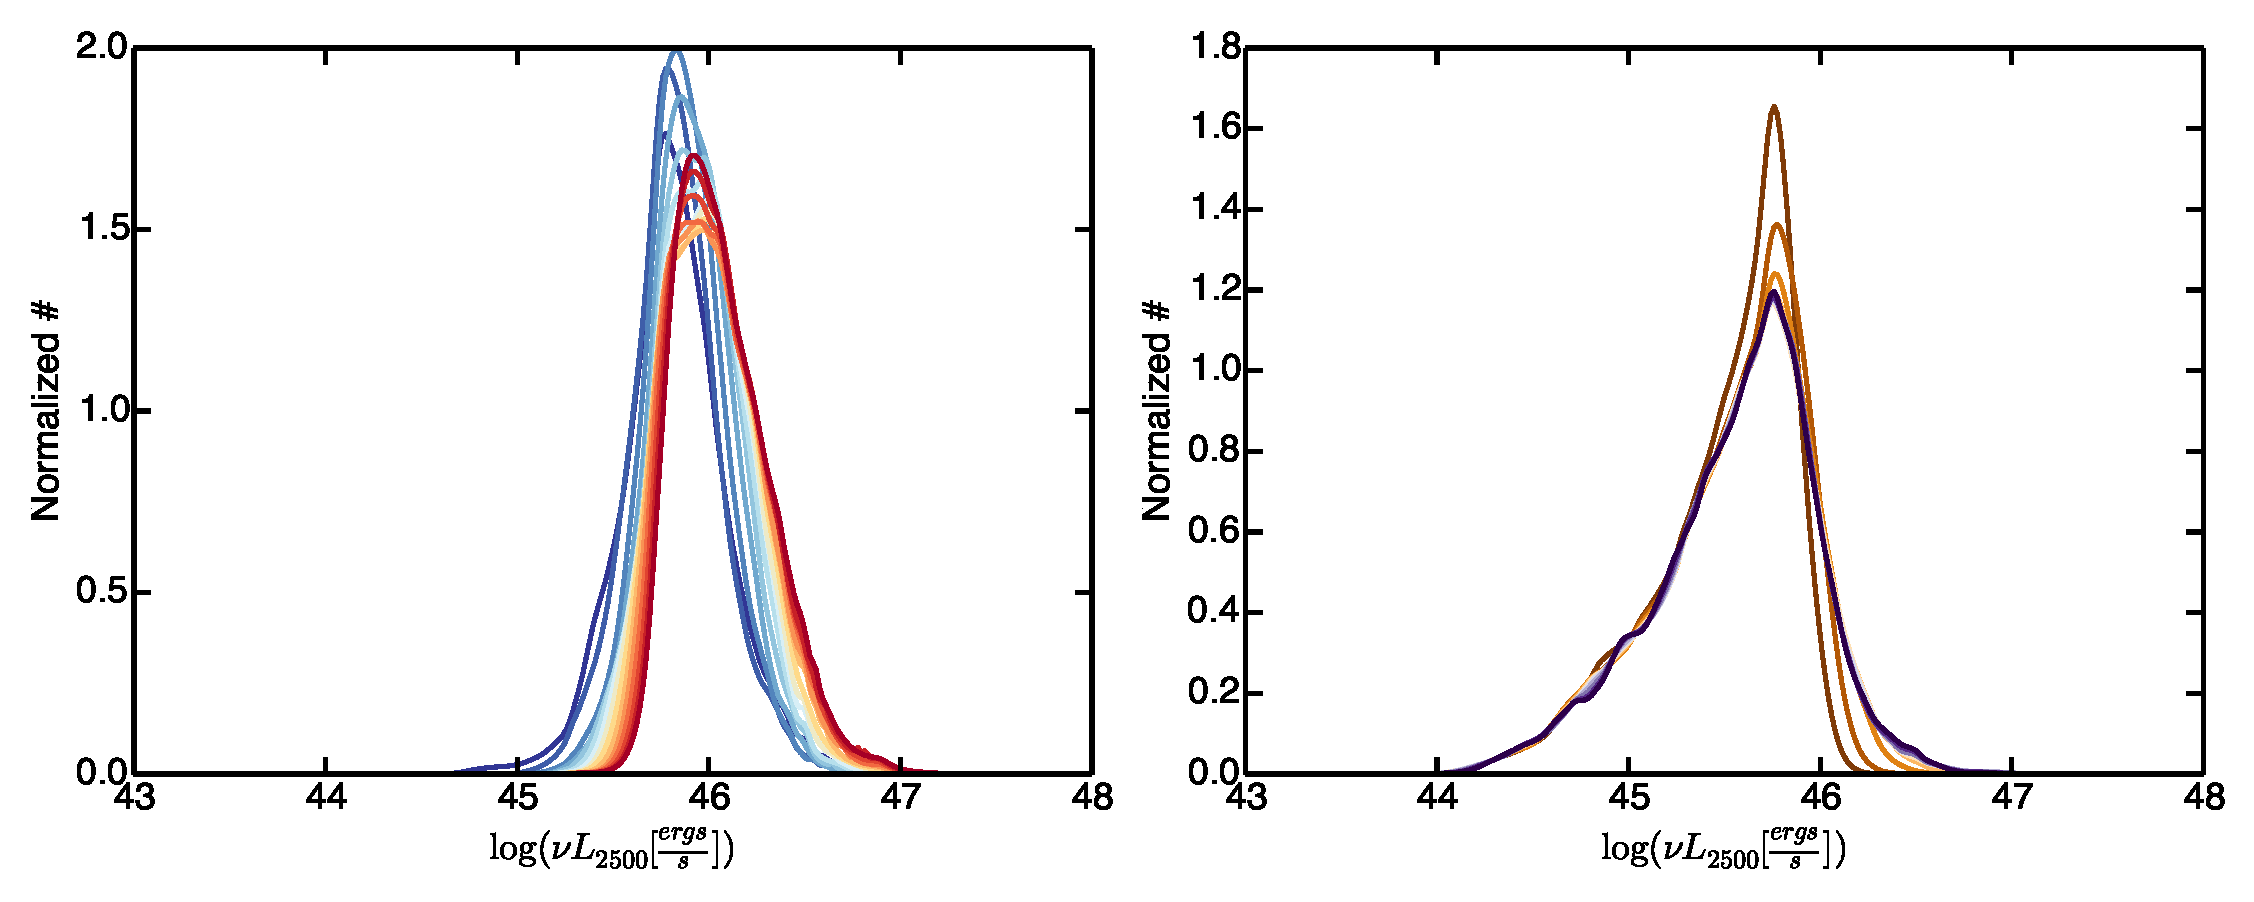
\includegraphics[width=\textwidth]{../images/BH/f8a}\\
		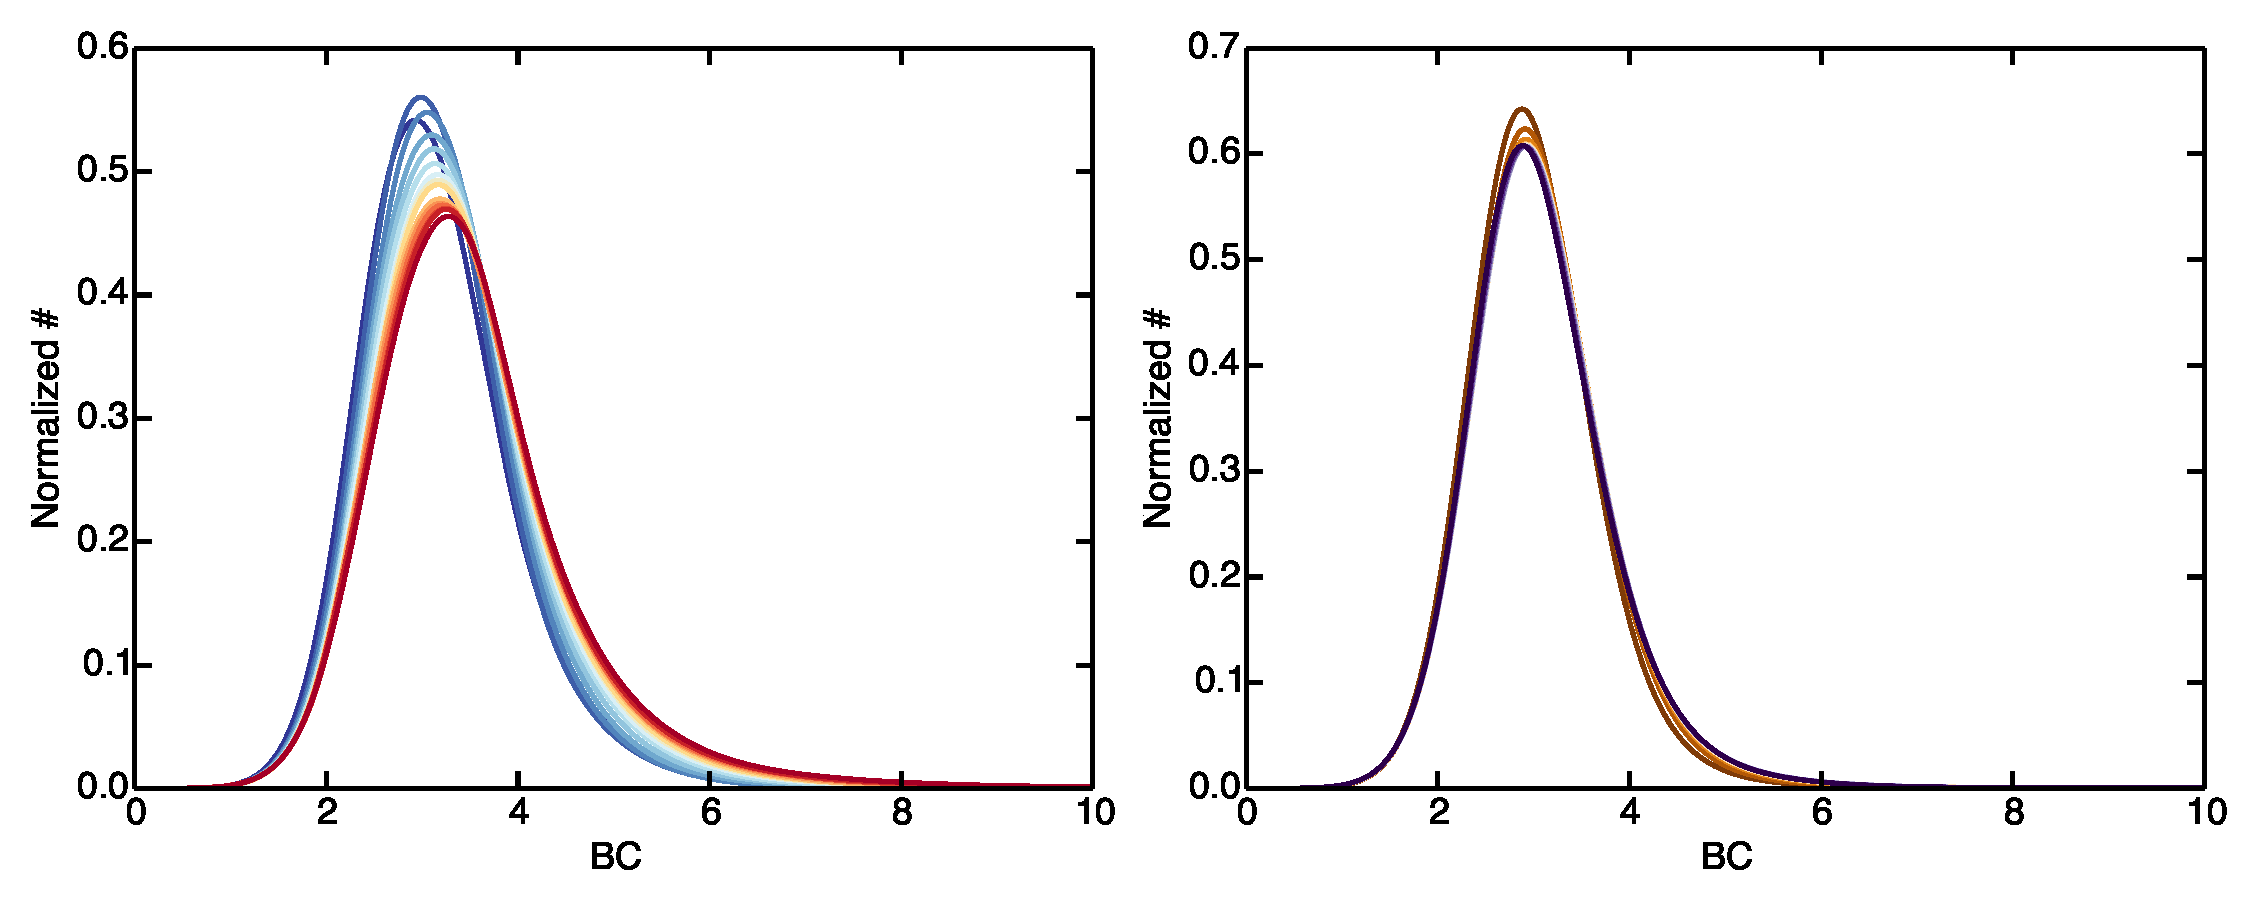
\includegraphics[width=\textwidth]{../images/BH/f8b}\\
		\hspace{2mm}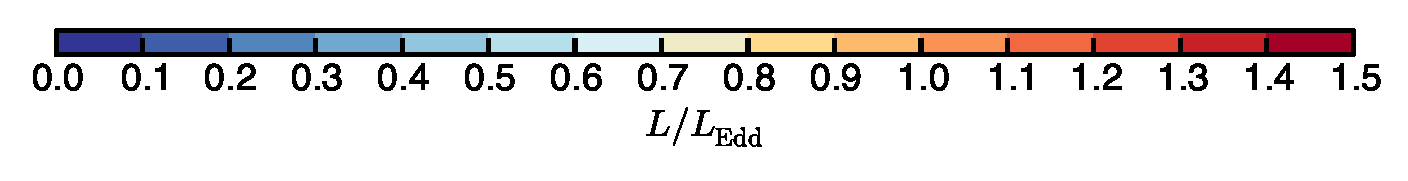
\includegraphics[width=.47\textwidth]{../images/BH/Lf_colorbar} 
		\hspace{2.5mm}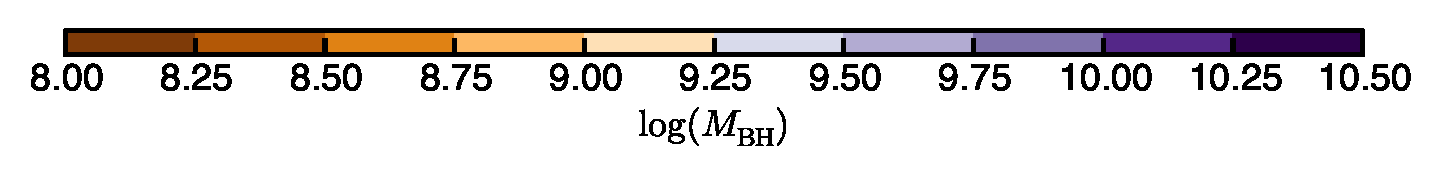
\includegraphics[width=.47\textwidth]{../images/BH/M_colorbar}
	\end{column}
	\end{columns}
\end{frame}
\end{document}